%SAVEDAT= 1453457093
\documentclass[11pt, a4paper]{article} 
\usepackage{slashed,jheppub,multirow,relsize,soul}
\usepackage[normalem]{ulem}
\usepackage{color}
\usepackage{subcaption}
\usepackage{mathabx}
\usepackage[utf8]{inputenc} 

\newcommand{\refeq}[1]{Eq.~(\ref{#1})}
\newcommand{\refeqs}[2]{Eqs.~(\ref{#1})~and~(\ref{#2})}
\newcommand{\refeqss}[3]{Eqs.~(\ref{#1}), (\ref{#2})~and~(\ref{#3})}
\newcommand{\reffig}[1]{Fig.~\ref{#1}}
\newcommand{\reffigs}[2]{Figs.~\ref{#1}~and~\ref{#2}}
\newcommand{\refsec}[1]{Section~\ref{#1}}
\newcommand{\refapp}[1]{Appendix~\ref{#1}}
\newcommand{\reftab}[1]{Table~\ref{#1}}
\newcommand{\refref}[1]{Ref.~\cite{#1}}
\newcommand{\refrefs}[2]{Refs.~\cite{#1}~and~\cite{#2}}

\def\abelian{abelian}
\def\nonabelian{non-abelian}
\def\lagrangian{lagrangian}
\def\eg{\emph{e.g.}}
\def\ie{\emph{i.e.}}
\def\aka{\emph{a.k.a.}}
\def\muboone{MicroBooNE}
\def\icarus{Icarus}
\def\minerva{MINER$\nu$A}
\def\ster{\ensuremath N}

%%%%%%% A few editorial macros. %%%%%%%

\newcommand{\lorem}{ \textcolor[rgb]{0.8,0.8,0.8}{Lorem ipsum dolor sit amet, constetur
adipiscing elit, sed do eiusmod tempor incididunt ut labore et dolore magna
aliqua. Ut enim ad minim veniam, quis nostrud exercitation ullamco laboris nisi
ut aliquip ex ea commodo consequat. Duis aute irure dolor in reprehenderit in
voluptate velit esse cillum dolore eu fugiat nulla pariatur. Excepteur sint
occaecat cupidatat non proident, sunt in culpa qui officia deserunt mollit anim
id est laborum.}}

\newcounter{CommentCount}
\setcounter{CommentCount}{1}

\newcommand{\marcom}[2]{\textsuperscript{\textcolor{#1}{\theCommentCount}}\marginpar{\textsuperscript{\textcolor{#1}{\theCommentCount}}\textcolor{#1}{{\small#1: #2}}}\stepcounter{CommentCount}}

\newcommand{\newtext}[2]{\textcolor{#1}{\ul{#2}}}

% Add your own colour down here... 
\definecolor{PB}{rgb}{0.9,0,0}
\definecolor{MARK}{rgb}{0.612, 0.153, 0.69}

%%%%%%%%%%%%%%%%%%%%%%%%%%%%%%%%%%%%%%%


\title{MeV-scale sterile neutrino decays at the Fermilab Short-Baseline Neutrino program}

\author{Peter Ballett,}
\author{Silvia Pascoli}
\author{and Mark Ross-Lonergan}

\affiliation{Institute for Particle Physics Phenomenology, Department of
Physics, Durham University, South Road, Durham DH1 3LE, United Kingdom}

\emailAdd{peter.ballett@durham.ac.uk}
\emailAdd{silvia.pascoli@durham.ac.uk}
\emailAdd{mark.ross-lonergan@durham.ac.uk}

\abstract{
%
Nearly-sterile neutrinos with masses in the MeV range and below would be
inevitably produced in the beam of the Short-Baseline Neutrino (SBN) program at
Fermilab and subsequently decay into visible particles in its detectors. In
this article we study the potential for SBN to discover these particles. We
discuss the decays which will be visible at SBN in a minimal and non-minimal
extension of the Standard Model, and perform a simulation to compute the
parameter space constraints which could be placed in the absence of a signal.
%
We demonstrate that the SBN programme can extend existing bounds on well
constrained channels such as $\ster \rightarrow \nu l^+ l^-$ and $\ster
\rightarrow l^\pm \pi^\mp$ while, thanks to the strong particle identification
capabilities of liquid-Argon technology, also place bounds on often neglected
channels such as $\ster \rightarrow \gamma \nu$ and $\ster \rightarrow \nu
\pi^0$. 
%
Furthermore, we consider the phenomenological impact of improved event timing
information at the three detectors. If the light detection system employed by
SBND and ICARUS can achieve nano-second timing resolution, the effect of
finite sterile neutrino mass would be observable as events are expected to
arrive outside the neutrino beam-buckets. When combined with spectral energy
information SBN can significantly reduce its beam-correlated backgrounds, while
through the comparison of event timing distributions at near and far detectors,
it can also provide a smoking-gun signature for this class of models.
%
We stress throughout that this is a complementary new physics analysis to the
search for eV-scale oscillations, extending the BSM programme of SBN while
requiring no beam or detector modifications.
%
}

\begin{document} 

\maketitle

\section{Introduction}

The neutrino sector of the Standard Model (SM) is known to be incomplete. The
observation of oscillatory behaviour between neutrino flavour states
\cite{Fukuda:1998mi} suggests that neutrinos possess a mass matrix and that
this has off-diagonal terms in the flavour basis. There are many models that
have been invoked in the literature to explain this observation as well as the
lightness of neutrino masses, ranging from the ever popular see-saw mechanisms
\cite{Minkowski:1977sc, GellMann:1980vs, Mohapatra:1979ia} to radiative mass
generation \cite{Zee:1980ai,Babu:1988ki} or even more involved constructions
such as neutrino masses originating from extra-dimensions
\cite{ArkaniHamed:1998vp}.  It will ultimately be the role of phenomenology to
find ways to distinguish between potential candidate models, and explore what
can be deduced about the completion of the neutrino sector from the analysis of
contemporary experiments.
%
%Not all models of neutrino masses, however, lend themselves to such direct
%terrestrial experimental searches. For example, the canonical Type-I see-saw
%\cite{Minkowski:1977sc, GellMann:1980vs, Mohapatra:1979ia} suggests the
%existence of new particles with masses  around $10^{12}$--$10^{15}$ GeV, well
%beyond the limits of foreseeable direct production. 
%
A common, although not necessary, feature in Beyond the SM (BSM) models which
account\marcom{PB}{I rolled back account/accounts.} for neutrino masses is the
presence of sterile neutrinos, SM-gauge singlet fermions which couple to the
active neutrinos via Yukawa interactions.  After electroweak symmetry
breaking\footnote{We focus on mass eigenstates which are nearly sterile but mix
with small angles with the active ones. For simplicity, and following previous
literature, we call them ``sterile neutrinos'' throughout the text.}, these
particles are coupled bilinearly to the active neutrino fields, and in the mass
basis, we find an extended neutrino sector including new states with
mixing-suppressed gauge interactions. \emph{A priori} their mass and
interaction scales can span many orders of magnitude, leading to a wide range
of distinct observable phenomena.
%
One of the best known examples is the short-baseline oscillation signature
associated with a sterile neutrino mass around the eV-scale (see \eg\
\refref{Gariazzo:2015rra} for a recent review), which has been invoked to
explain anomalies found at some short-baseline oscillation experiments
\cite{Aguilar:2001ty, Aguilar-Arevalo:2013pmq, AguilarArevalo:2008rc}.
Explaining all anomalies in an economical fashion appears challenging in these
models \cite{Kopp:2013vaa,Conrad:2012qt}, but more data would be needed before
a decision can be made as to their role in the neutrino sector. The Fermilab
SBN \cite{Antonello:2015lea} program was primarily designed to perform such a
conclusive test.

The SBN experiment is comprised of three detectors placed in the Booster
Neutrino Beam (BNB) at different (short) baseline distances: SBND (previously
known as LAr1-ND) at 110~m from the target, \muboone\ at 470~m and ICARUS at
600~m.  All three detectors employ Liquid Argon Time Projection Chamber
(LArTPC) technology \cite{Rubbia:1977} with strong event reconstruction
capabilities allowing for a significantly improved understanding of background
processes compared to predecessor technologies. 
%
With this design SBN has been shown to be able to extend the current bounds on
oscillatory sterile neutrinos, thoroughly exploring the eV-scale sterile
neutrino mass region, whilst also pursuing many other physics goals
\cite{Antonello:2015lea}.

In this article, we assess the potential for SBN to contribute to the search
for sterile neutrinos in a manner complementary to the oscillatory analysis.
The new fermions in our study are assumed to have masses around the MeV scale.
These particles are light enough to be produced in neutrino beams via meson
decay, but have masses sufficiently large to prevent oscillatory effects with
the active neutrinos through loss of coherence (see \eg\
\refref{Akhmedov:2009rb}), instead propagating long distances along the
beamline. Due to the presence of mixing they are unstable, and their
subsequent decay products can be observed in neutrino detectors.
%
%have been enumerated \cite{Atre:2009rg} and searched for in many previous
%experiments.
%
%The focus of this paper will be on estimating the sensitivity of the SBN
%program to sterile neutrinos produced in this way.
%
We stress that the search for MeV-scale sterile neutrinos is entirely
compatible with the primary goals of SBN, and requires modification of
neither the beam nor detector designs. 

%Given the existing anomalies in short baseline neutrino experiments, including
%MiniBooNE which also operated in the BNB, the possibility of seeing an
%anomalous signature at the SBN complex should not be ignored. It is therefore
%timely to ask how we can extract the physical content of such an excess, and
%we present ways that such decaying steriles can be identified or excluded.

The reconstruction \cite{Church:2013hea, Marshall:2015rfa}, energy resolution
\cite{Sorel:2014rka} and excellent calorimetric particle identification
capabilities of LAr \cite{Antonello:2012hu} technology means the SBN program
provides an ideal scenario to study this ``decay-in-flight'' of sterile
neutrinos.  This allows for a high degree of background suppression on well
studied decay modes while also allowing the study of channels which have been
poorly bounded by similar experiments due to large backgrounds and challenging
signals. For example, the differentiation between an electron- or photon-
induced EM shower can be achieved by studying their rate of energy loss in the
first 3cm of their ionising track \cite{szelc:2007}. Furthermore, as we
discuss in \refsec{sec:timing}, if a sufficiently good timing resolution of
scintillation light is achieved, the timing structure of markedly sub-luminal
sterile neutrinos can be utilised as both a rejection mechanism for beam
related backgrounds as well as a further aid for model discrimination and mass
measurement.

\begin{table}[t!]
\centering
\begin{tabular}{| l || l | l | l | l |}
	\hline
	& PS-191 & SBND & MicroBooNE & ICARUS \\ \hline \hline
	POT	& $0.86 \times 10^{19}$	& $6.6 \times 10^{20}$	&	$13.2 \times 10^{20}$     &  $6.6 \times 10^{20}$ \\ \hline
	Volume	& $216\text{m}^3$	&	$80\text{m}^3$	&	$62\text{m}^3$	     &   $340\text{m}^3$	\\ \hline
	$\text{Baseline}^{-2}$	& $(128 	\text{m} )^{-2}$	&$(110 \text{m} )^{-2}$	&	$(470 \text{m} )^{-2}$			     & $(600 \text{m} )^{-2}$	  \\ \hline
Ratio/PS-191 & - 	& 38.5 	& 3.3	& 5.5\\ \hline
	S/$\sqrt{B}$ Ratio & - 	& 16.3 	& 1.8	& 1.1\\ \hline
\end{tabular}

\caption{\label{tab:exposure} A comparison of the relative exposure at each SBN detector
compared to PS-191. One would expect all  three SBN detectors to see increased
numbers of events than PS-191 did, with SBND seeing the largest enhancement of a
factor of $38.5$. The final row takes into account the scaling in masses
leading to increased backgrounds, although the achievable reconstruction of LAr
should reduce these significantly.}

\end{table}

We restrict our analysis to sterile neutrino masses below the kaon mass, for
which there is significant energy in the proton beam to produce in high
numbers. In this mass range, the strongest bounds on sterile neutrinos which
mix with electron and muon neutrinos come from PS-191 \cite{Bernardi:1985ny,
Bernardi:1987ek}, a beam dump experiment which ran at CERN in 1984. 
%
PS-191 was constructed from a helium filled flash chamber decay region,
followed by interleaved iron plates and EM calorimeters. It was located 128~m
downstream of a Beryllium target and $2.3^\circ$ (40 mrads) off axis, obtained
$0.86 \times 10^{19}$ POT over the course of its run-time, and had a total
detector volume of $6\times3\times12 = 216 \text{m}^3$. We can estimate the
sensitivity of the three SBN detectors and how they will compare to PS-191 by
estimating the experiments' \emph{exposure}, defined here as POT $\times$ Vol
$\times$ $R^{-2}$. We compare the three detectors to PS-191 in
\reftab{tab:exposure}, which indicates that all detectors of the SBN complex
expect a larger exposure, with SBND seeing the greatest enhancement by a factor
of around $40$. 
%
In addition to the larger exposure, there is also an enhancement of the
expected decay events at SBN due to its lower beam energy. The sterile
neutrinos at SBN are produced by the 8 GeV BNB beam and have a softer spectrum
than those produced by the 19.2 GeV CERN Proton Synchrotron beam used at
PS-191. As we discuss in more detail in \refsec{sec:decays}, the probability
that the sterile neutrino decays inversely scales with momentum, $1/|P_\ster|$,
and we would therefore expect any BNB detectors to see more events than PS-191
for equivalent neutrino exposures.

However, exposure alone does not dictate sensitivity. PS-191 was purposefully
built to search for decays of heavy fermions. To minimise the background
induced by active neutrino scattering, the total mass of the detector (and
therefore number of target nuclei) was chosen to be small (approximately $20$
ton). Conversely, the SBN detectors were designed to search for neutrino
interactions and thus have significantly larger masses ($112$, $66.6$ and $476$
tons respectively). SBN will not only see a greater number of decay events than
PS-191 but also a greater background for a given exposure. Therefore, the
degree of background reduction will be crucial in determining its ultimate
performance. We return to this issue in \refsec{sec:backgroundestimate}.

The paper is structured as follows. In \refsec{sec:decays} we present an
overview of sterile neutrino decay in minimal and non-minimal models relevant
for beam dump experiments. We then present the details of our simulation in
\refsec{sec:simulation} and show illustrative event spectra from out simulation
for some channels of interest. In \refsec{sec:sensitivities}, we discuss the
exclusion contours that SBN could place on the model in the absence of a
signal. We then study how the event timing information could be used to prove
any observed excess is indeed originating in such a decay-in-flight scenario
and help constrain the particle masses if a positive signal were indeed
detected. We make some concluding remarks in \refsec{sec:conclusions}.

\section{\label{sec:decays}Sterile neutrino production and decay}

The most general renormalizable \lagrangian\ extending the SM to include a new
gauge-singlet fermion $\ster$ is given by
%
\begin{align}   \mathcal{L}_N = \mathcal{L}_\text{SM} +
\overline{\ster}i\slashed{\partial}\ster + \left(\frac{m_\ster}{2}
\overline{\ster^\text{c}}\ster  + y_\alpha\overline{L}_\alpha\widetilde{H}
\ster + \text{h.c.}\right),\label{eq:minimallag} \end{align}
%
where $N^c=C\overline{N}^\text{T}$ with $C$ denoting the charge-conjugation
matrix, $L_\alpha$ is the SM leptonic doublet of flavour $\alpha$, $y_\alpha$
represents the Yukawa couplings and $m_\ster$ a Majorana mass term for $\ster$.
The extension to multiple new fermions involves promoting $y$ and $m_\ster$ to
matrices with indices for the new states, but will offer no real
phenomenological difference in the following analysis.\footnote{The minimal single
$\ster$ extension does not allow for the observed masses of the neutrinos, as
the mass matrix is rank 1. We assume that an appropriate extension has been
introduced to satisfy neutrino oscillation data while introducing no new
dynamics at the lower energy scales of interest.} Much work has been done
understanding the phenomenology of such novel neutral states, which varies
significantly over their large parameter spaces. 
%
Lagrangians similar to this have been used in the literature for a wide range
of purposes. If the new particle has a mass around $10^{12}$-$10^{15}$ GeV it
could provide a natural way to suppress the size of active neutrino masses
through the Type I or III see-saw mechanisms \cite{Minkowski:1977sc,
GellMann:1980vs, Mohapatra:1979ia}. A lighter neutral fermion, with a mass
around the keV scale, remains a promising dark matter candidate
\cite{Adhikari:2016bei}. A synthesis of these ideas is found in the so-called
$\nu$MSM which simultaneously can explain dark matter, neutrino masses and
successful baryogenesis \cite{Asaka:2005pn}. 
%
If the sterile neutrino gets lighter still, with masses at the eV scale or
below, the particles can alter the neutrino oscillation probability, leaving
observable signatures at oscillation experiments. Indeed, such particles have
been proposed to alleviate short-baseline oscillation anomalies; although, no
minimal solution seems to provide a compelling universal improvement to the
current data \cite{Kopp:2013vaa,Conrad:2012qt}.

A key feature of models of sterile neutrinos are the weaker-than-weak
interactions which arise from mass mixing. In the minimal \lagrangian\ in
\refeq{eq:minimallag}, the only direct couplings to new sterile flavour
eigenstates are neutrino--Higgs interactions. However, these couplings generate
off-diagonal neutrino bilinears below the electroweak symmetry breaking scale,
leading to mixing-mediated interactions with SM gauge bosons for the mostly
neutral mass eigenstate. This allows them to be produced in and decay via SM
gauge interactions, albeit suppressed by the mixing angle. 

The possibility remains that extra particles exist beyond the minimal
\lagrangian\ and these mediate other interactions, either directly with SM
fields or, as before, via mixing. 
%
Throughout our work, we assume that the production of $N$, described in
\refsec{sec:prod}, is generated by the interactions in \refeq{eq:minimallag}.
However, we will return to the idea of a non-minimal \lagrangian\ in
\refsec{sec:nonminimal} when discussing the decay modes of $N$.

\subsection{\label{sec:prod}Production at BNB}

For sterile neutrinos which are light enough to be produced from a meson beam,
there is a qualitative divide in the phenomenology somewhere between keV and eV
masses\footnote{The precise mass range depends on details of the process under
consideration.}. If the sterile neutrinos are massive enough for their
mass-splittings with the light neutrinos to be larger than the wavepacket
energy-uncertainty associated with the production mechanism, they no longer
oscillate \cite{Akhmedov:2009rb}.  
%
%Once oscillation is suppressed, 
%
Neutral particles produced in the beam will propagate towards the detector and
may be observed by their subsequent decay into SM particles. Experiments
seeking to measure such decays are generally known as beam dump experiments,
where proton collisions with a target produce particles to be observed
down-wind of the source \cite{CooperSarkar:1985nh, Bergsma:1985is,
Vaitaitis:1999wq, Bernardi:1985ny, Bernardi:1987ek, Anelli:2015pba,
Alekhin:2015byh}. It has been pointed out that the difference between a beam
dump and a conventional neutrino beam is more a matter of philosophy than
design, and we can expect many experiments to have some sensitivity to novel
heavy states \cite{Gorbunov:2007ak, Asaka:2012bb, Adams:2013qkq}. 
%
For the BNB, we can estimate the mass at which the oscillatory behaviour is
suppressed as follows: the decay pipe for BNB is around $50$~m in length, which
is considerably shorter than the decay lengths of the mesons in the beam, and
we assume that this length defines the wavepacket width at production.  The
relevant parameter is the decoherence parameter \cite{Akhmedov:2009rb,
Hernandez:2011rs}
%
$\xi = 2\pi \frac{\lambda_\text{d}}{\lambda_\nu},$
%
where $\lambda_\text{d} = 50$~m and $\lambda_\nu$ is the standard neutrino
oscillation length $\lambda_\nu = \Delta m^2/4E_\nu$. For $\xi\gg1$ the wave
packet is insufficiently broad to accommodate a coherent superposition of the
heavy and light neutrino states. We estimate that this occurs for the BNB at 
%
$ \Delta m^2 \gtrsim 100~\text{eV}^2.$
%
%In this article we study the region of MeV scale sterile masses. These are
%heavy enough to forbid oscillatory effects while light enough to be have
%significant production from the meson decays associated with a conventional
%neutrino beam. 

In a conventional neutrino beam, most neutrinos are derived from meson decay,
and we assume in this work that the sterile neutrinos are produced from the
decays of pions and kaons, restricting our sterile neutrino mass to $m_\ster \le m_K$.
%
Larger sterile neutrino masses could be probed by working at higher energies in the
initial proton beam, where the neutral fermions could come from decays of
charmed mesons such as $D^\pm$. This strategy will be used by the upcoming
SHiPS experiment \cite{Alekhin:2015byh, Anelli:2015pba} but will not be
considered further in the present work as $D$ mesons are produced in extremely
small numbers due to the relatively low energy of the BNB beam
\cite{AguilarArevalo:2008yp}. As such we restrict ourselves to the naturally
defined mass range of interest for SBN, eV $\gg m_\ster \lesssim$ 494~MeV.  We
focus on $m_\ster \geq$ MeV scale states where the prospects for detection are
greatest due to enhanced decay rates.

%
Although novel dynamics may lead to enhanced production rates of sterile
neutrinos by alternative unconventional means, we neglect this possibility and
assume that the sterile component of the BNB flux arises solely from meson (or
secondary $\mu^\pm$) decays. This process requires only mass-mixing from the
$N$-$\nu$ Yukawa term in \refeq{eq:minimallag}. It follows that the amplitudes
for these decays are related to those of the standard leptonic decays of mesons
via an insertion of the mixing matrix element $U_{\alpha 4}$, and to leading
order in the mass of the sterile neutrino over the meson mass, the
$\ster$-fluxes will be a rescaling of the fluxes for the active neutrinos. 
%
However in order to account for flavour-specific effects, it is necessary to go
beyond this approximation and consider the kinematic differences of heavy
sterile neutrino production.
%
The flux of sterile neutrinos produced from the decay of a given meson $M$ is
approximated by
%
\begin{equation} \phi_{\ster}(E_{\ster}) \approx \phi_{\nu_\alpha} (E_{\nu_\alpha})\vert
U_{\alpha 4}\vert^2 \frac{\rho\left( \delta_M^a , \delta_M^i
\right)}{\delta_M^a \left(1- \delta_M^a\right)^2}, \label{eq:flux_approx} \end{equation}
%
where $\rho(a,b)=\mathcal{F}_M(a,b) \lambda^{\frac{1}{2}}(1,a,b)$ is a
kinematic factor consisting of a term proportional to the two body phase space
factor, $\lambda(x,y,z)=x^2+y^2+z^2-2(x y+yz+x z)$ and a term proportional to
the matrix element, $\mathcal{F}_M(a,b)= a+b -\left(a-b\right)^2$, with
$\delta_M^{a(i)}=m_{l_a(\nu_i)}^2/M^2$ \cite{PhysRevD.24.1232}. 

The kinematic factor leads to two effects. First, it provides a threshold effect
of suppressing the production when the phase space decreases near a kinematic
boundary.  Secondly, it allows for the helicity un-suppression of channels
which in a conventional beam are highly suppressed. For example, the decay
$\pi^\pm \to e^\pm \nu_e$ which is significantly suppressed compared to the
comparable muonic channel, sees no such suppression when the neutrino is
replaced with $N$.
%
This kinematic effect for the pion and kaon can be substantial, for $\pi
\rightarrow e \nu$ this factor can be as large as $10^5$, which more than
compensates for the significantly smaller intrinsic flux of $\nu_e$ inherent in
the BNB, $\approx 0.52$\% \cite{AguilarArevalo:2008yp}. The approximation in \refeq{eq:flux_approx}
starts to fail as the mass of the sterile neutrinoincreases, and we begin to
see components of the active flux having energies less than the sterile mass
which are truncated by the kinematic factor. In order to keep the normalisation
of total neutrino events constant, before $U_{\alpha 4}$ and kinematic scaling,
any events which are below the sterile neutrino mass threshold are removed and the
remaining flux is scaled accordingly.

%The final sterile fluxes can be estimated by taking known active neutrino
%fluxes and scaling them by the appropriate mixing $U_{\alpha 4}$, with an
%additional kinematic factor to take into account the helicity un-suppression of
%channels if the flavour pattern allows, such as $\pi^+ \rightarrow e^+\ster$
%for massive $\ster \gg m_e$ if $U_{e4}$ is non-zero. 
%
%As mentioned in the introduction, because the meson decay comes with an
%associated charged lepton, mixing with the $\tau$-flavour cannot lead to
%production at the BNB, and so production is only possible with $U_{e4}$,
%$U_{\mu 4}$ or a combination of the two.

\begin{figure}[t]
\centering
\begin{subfigure}{.5\textwidth}
  \centering
  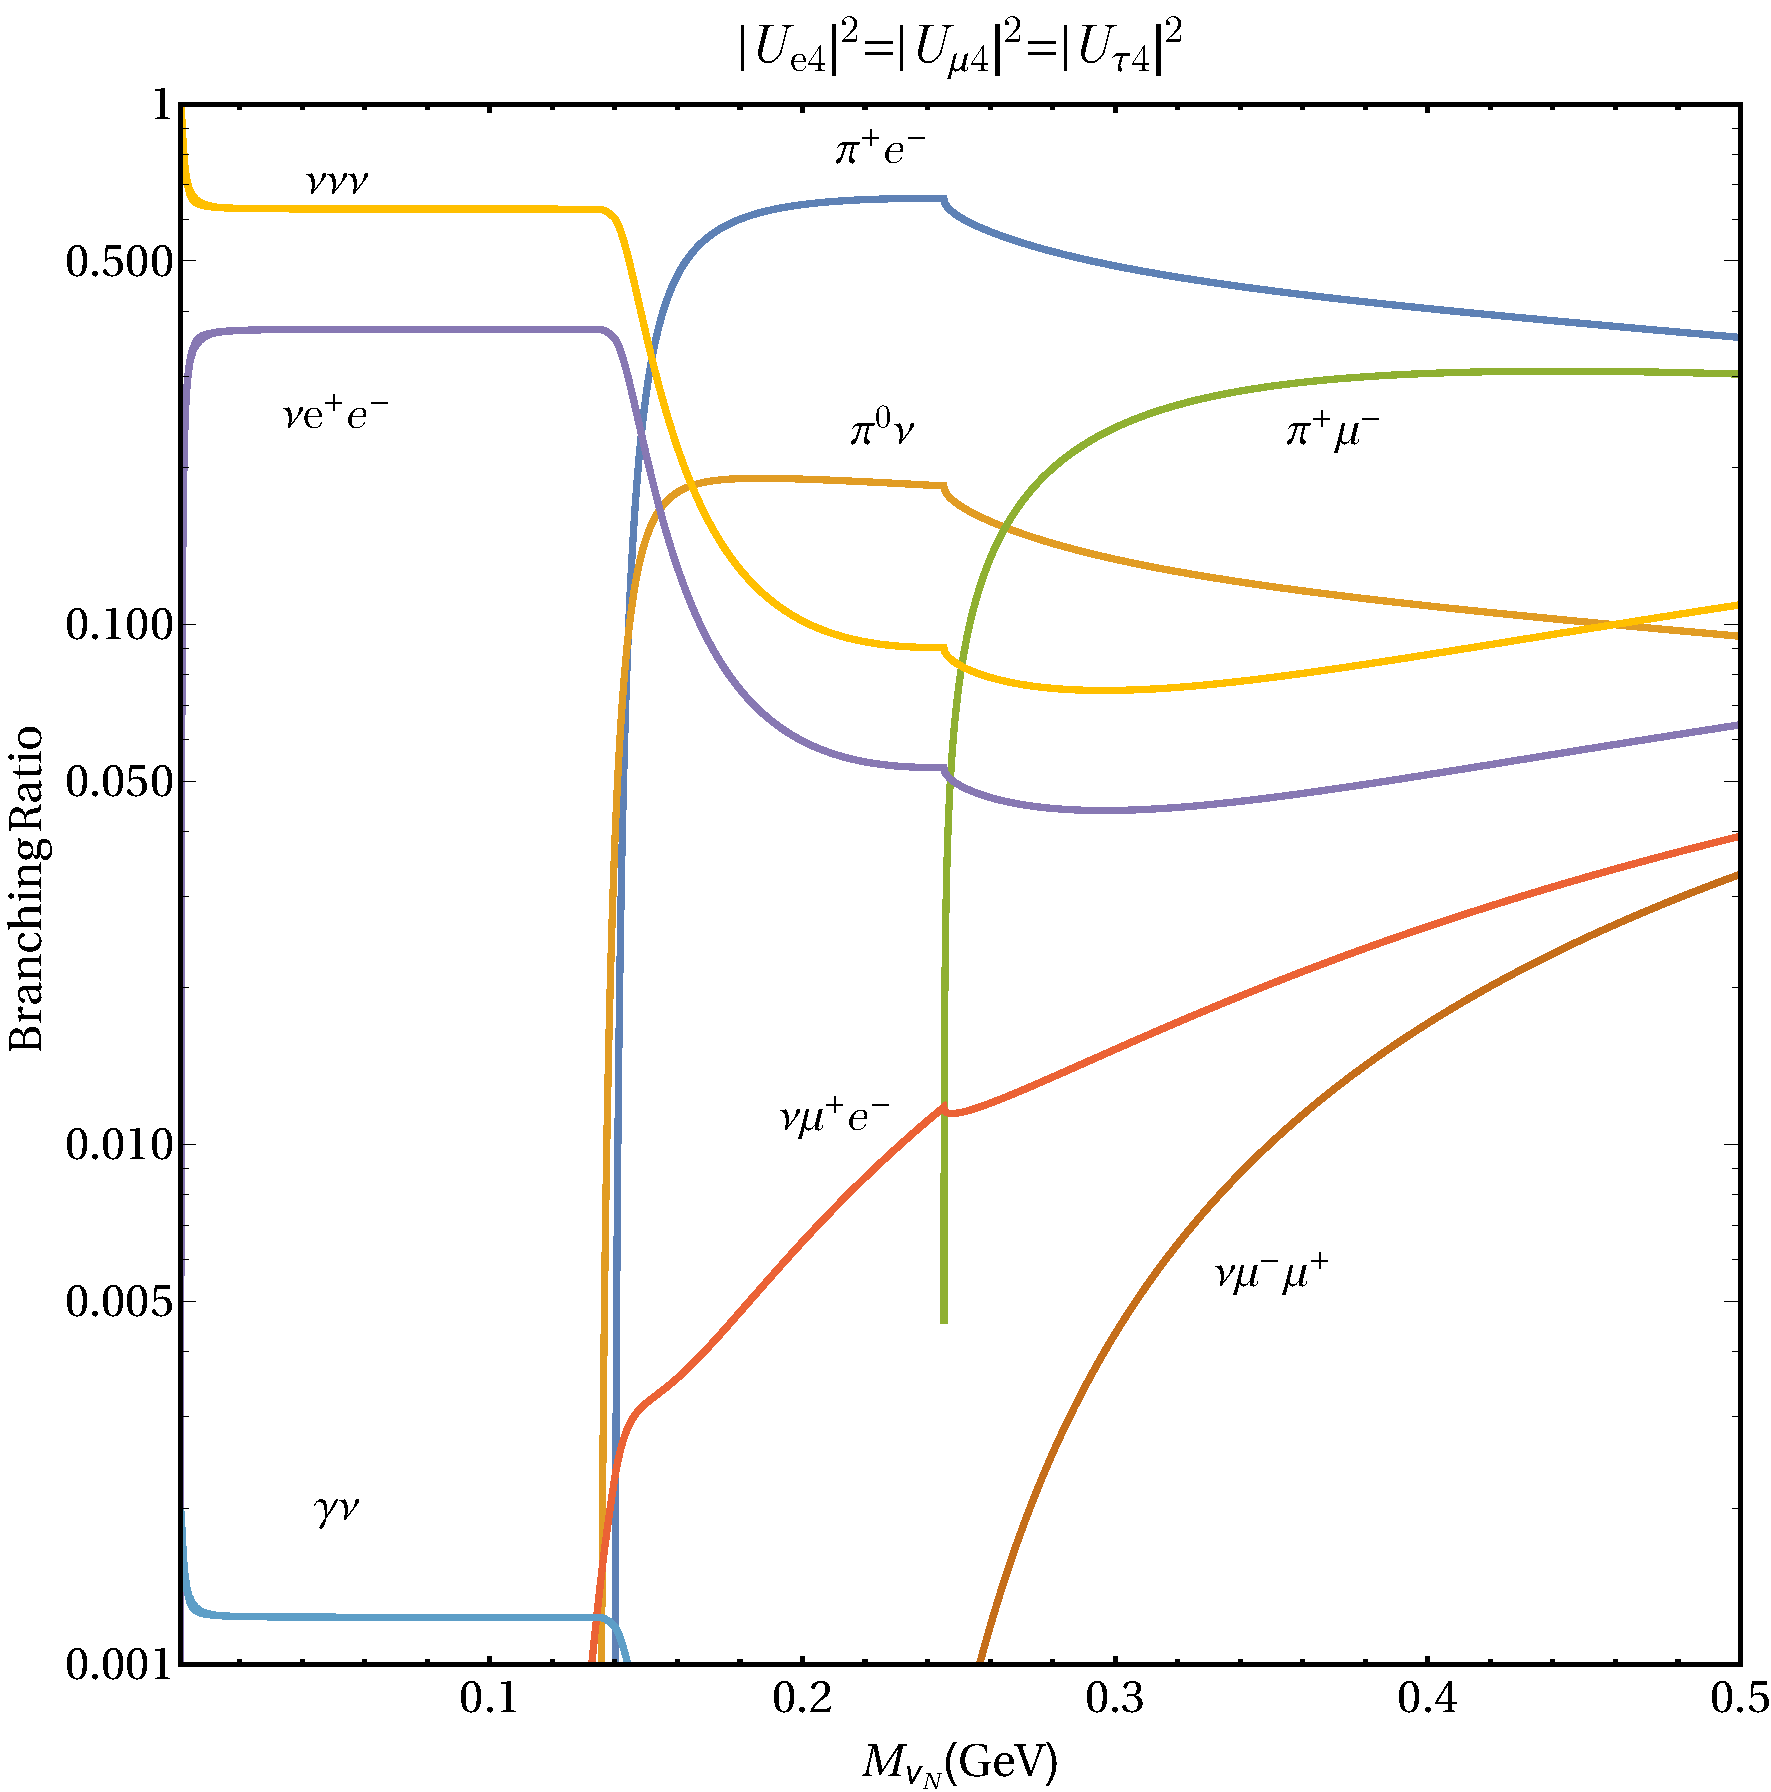
\includegraphics[width=\linewidth]{figures/BR_notlog_square.pdf}
\end{subfigure}%
\begin{subfigure}{.5\textwidth}
 \centering
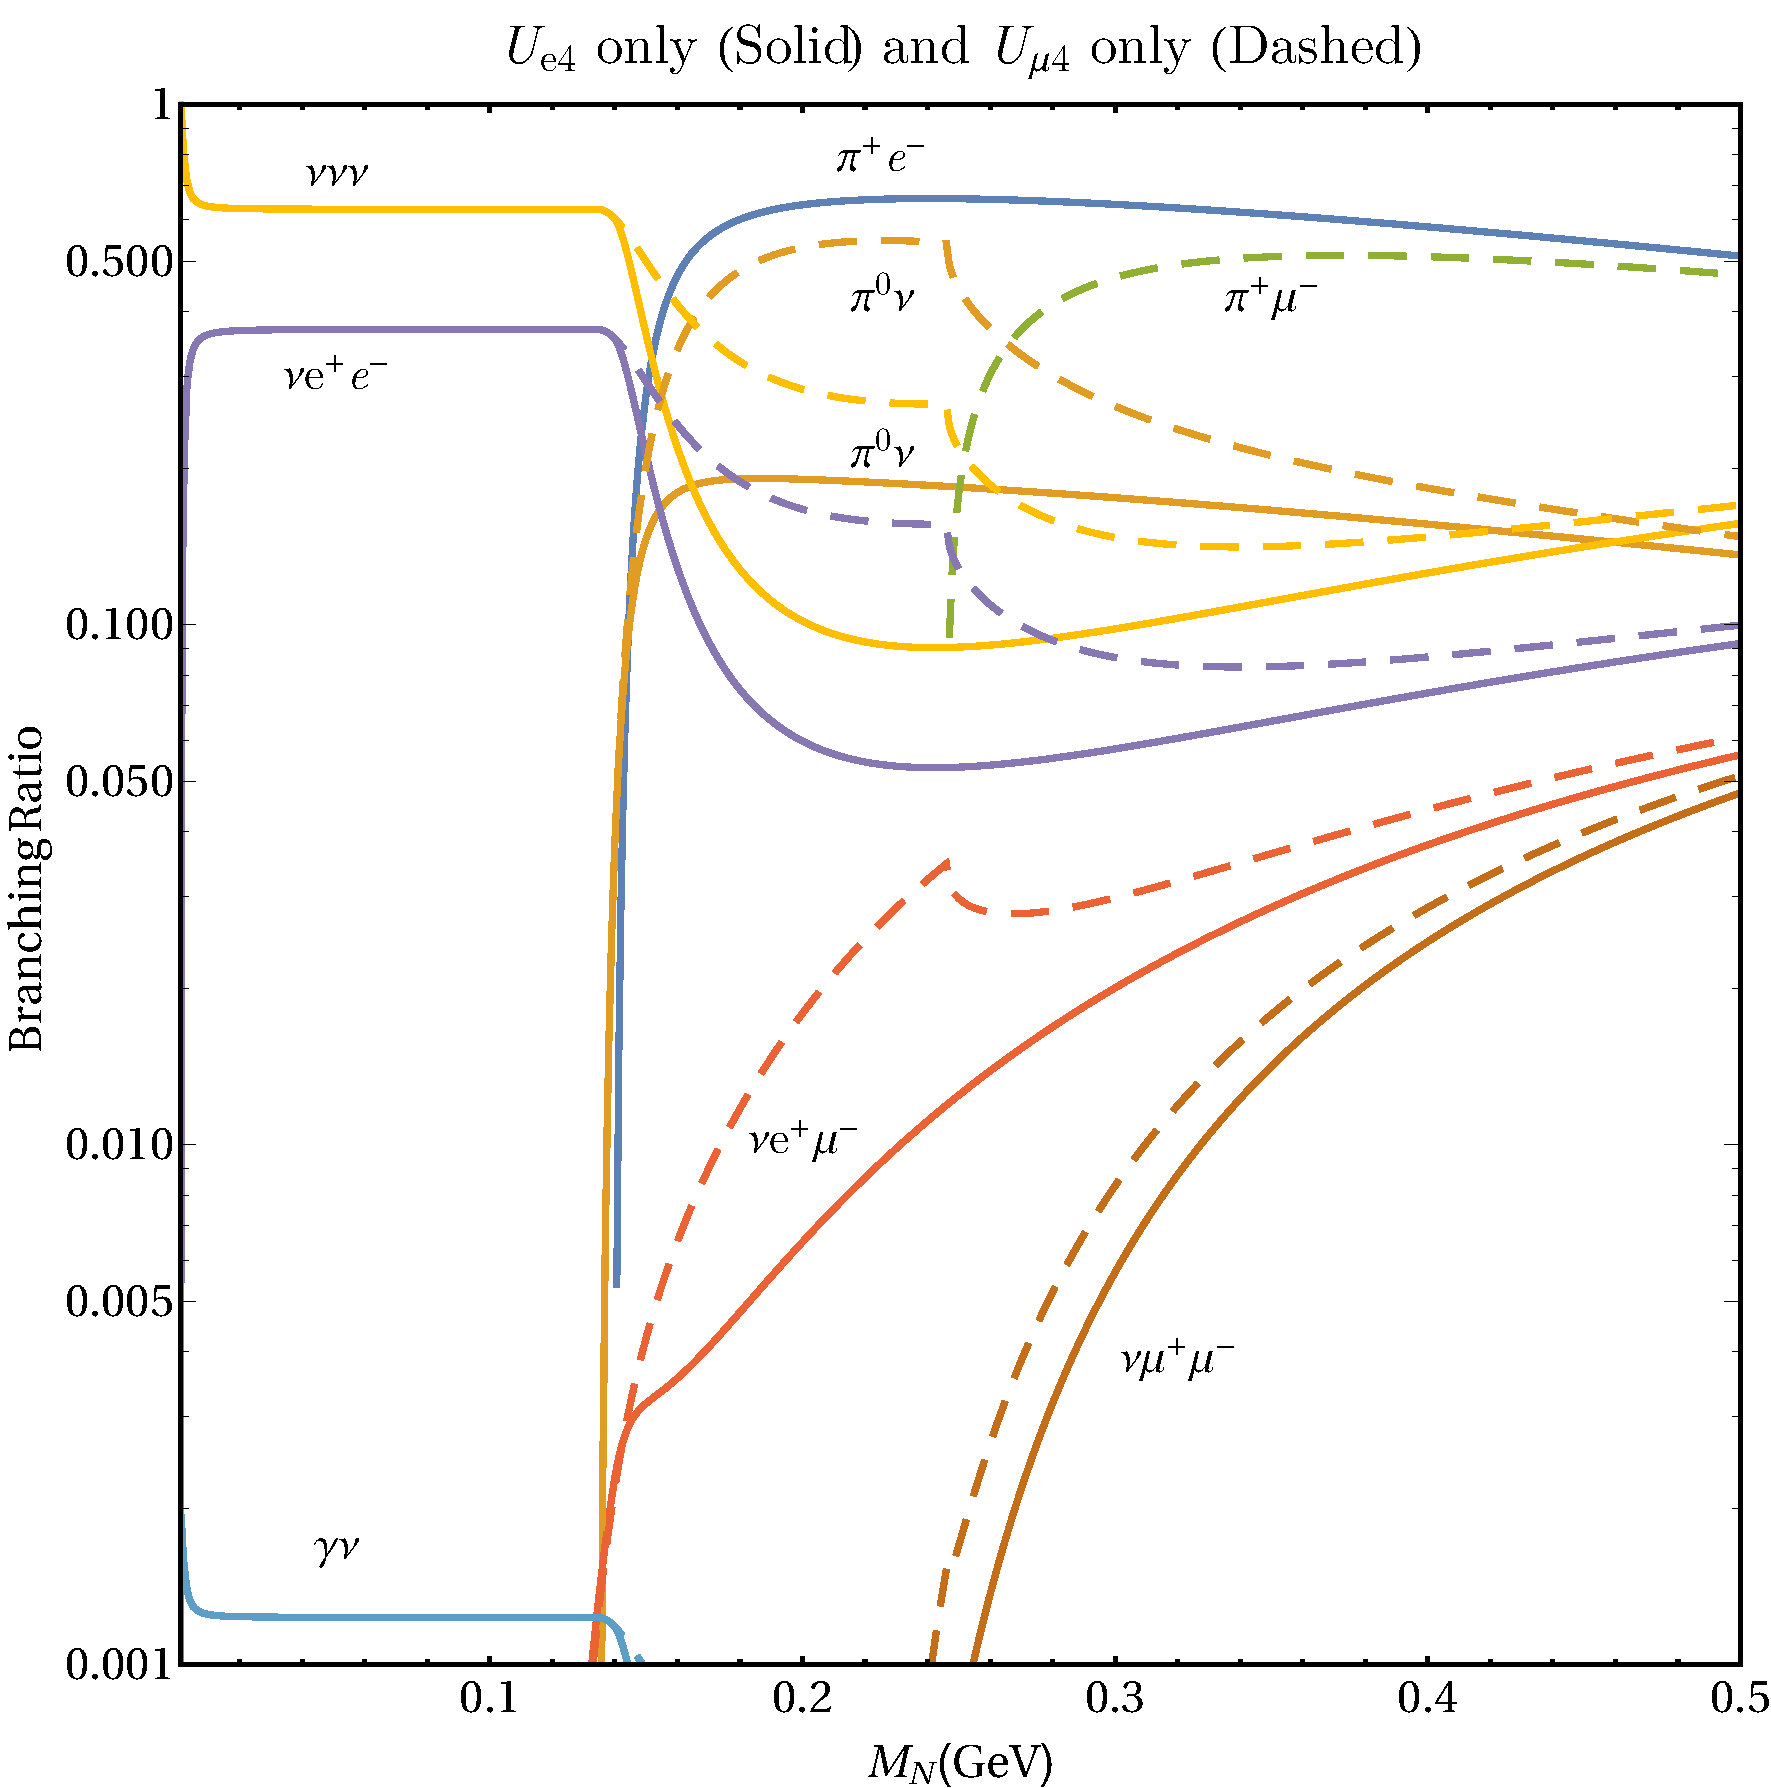
\includegraphics[width=\linewidth]{figures/BR_notlog_square2.pdf}
\end{subfigure}

\caption{\label{fig:branchingratios}The branching ratios for sterile neutrino
decays in the minimal 3 sterile neutrino SM extension, with masses between 1
MeV and 0.5 GeV. We assume both a flavour independent mixing pattern (\emph{left}) 
and a hierarchical scenario in which either $U_{e4}$ (solid lines) or $U_{\mu 4}$
(dashed lines) is only non-zero (\emph{Right}). Heavier sterile neutrinos will
not be produced in great numbers in the BNB beam due to the very small
component of heavier mesons in the secondary beam \cite{AguilarArevalo:2008yp}.
Note that below 100 MeV, in all scenarios, $\ster \rightarrow \nu_\alpha e^+
e^-$ is by far the dominant visible decay and, as such, is a key channel to 
constrain these models.}

\end{figure}
%

\subsection{Decay at SBN}

The fermions $N$ will generally be unstable, albeit possibly long-lived, allowing
for decays-in-flight into SM particles. In this work, we try to keep an open
mind about the interactions of the sterile neutrino and consider all
kinematically possible tree-level decays to visible SM particles for sterile
fermions produced by pion and kaon decays, $10~\text{MeV}\lesssim m_{\ster}
\lesssim m_K$. The precise decay rates and branching ratios for these channels
are model dependent. 
%

%These are shown schematically in \reffig{fig:decaydiagrams}.
%
%\begin{figure}[t] \begin{align*} \pi^\pm / K^\pm \longrightarrow
%\overbrace{l^\pm \ster}^{\text{via } U_{e4} \text{ or } U_{\mu 4}}
%&\longrightarrow \left. l^\pm \pi^\mp, \qquad \right\} \text{via } U_{e4}
%\text{ or } U_{\mu 4}\\ & \drsh \nu_\alpha l^+ l^-,\\[\jot] & \drsh \nu_\alpha
%\gamma   ,\hspace*{3em}
%\smash{\left.\begin{array}{@{}c@{}}\\[\jot]\\[\jot]\\[\jot]\end{array}\right\}}\text{via
%} U_{e4}, U_{\mu 4} \text{  or  } U_{\tau 4}\\[\jot]
%& \drsh \nu_\alpha \pi^0.  \end{align*}
%
%\caption{\label{fig:decaydiagrams}The production and decay channels considered
%in this study, where $l$ referes to either $e^+e^-$, $\mu^+ \mu^-$ or $\mu^\mp
%e^\pm$. }
%
%\end{figure}
%
\subsubsection{\label{sec:minimal}Minimal model}

We define the minimal sterile neutrino model by the Lagrangian in
\refeq{eq:minimallag}. This corresponds to the best known model of sterile
neutrino phenomenology: the UV-complete Type I see-saw (and its low-scale
variants). 
%
%but would also well describe other extensions of the SM with fields and
%symmetries not directly affecting the neutrino sector.
%
Decays of sterile neutrinos in such a model proceed via SM interactions
suppressed by the mixing angle and have been studied in \refref{Atre:2009rg,
PhysRevD.24.1232, PhysRevD.24.1275}. We have plotted the branching ratios
for sterile neutrinos in our mass range in \reffig{fig:branchingratios}, and 
we will now briefly summarise the decay rates most important for the present
study.

The decays of the minimal model depend only on the mass of the $\ster$ and the
size of neutrino mixing to various flavours, parameterized by the elements of
an extended PMNS matrix, \emph{e.g.} for one additional particle 
%
$U_{\alpha 4}$ for $\alpha \in \{e,\mu,\tau\}$. 
%
The branching ratios for these decays are shown in \reffig{fig:branchingratios}
as a function of mass for two sets of assumptions about the PMNS matrix. On the
left, we show the branching ratios if all mixing elements are of a similar
size, whereas on the right we assume that only $U_{\mu4}$ or $U_{e4}$ are
non-zero. This leads to certain decays being forbidden; for example, without
the coupling to the electron $U_{e4}=0$, the dominant channel for masses
$m_{\pi^0}~\lesssim m_\ster \lesssim m_{\mu}+m_{\pi^\pm}$ will be into a
neutral pion and a neutrino.\marcom{PB}{Added this back. I see this as a little
foreshadowing: we claim LAr can measure this and that it is relevant for the
first time with SBN!}

For sterile neutrino masses less than the pion mass, the dominant decay is into
three light neutrinos. This channel is for all practical purposes unobservable
and we will not consider it further. The dominant decay into \emph{visible}
particles will be into an electron-positron pair with a branching fraction of
around $38\%$. 
%
This is true regardless of the flavour structure of the mixing matrix;
although, this decay channel is not flavour-blind. If the sterile neutrino
mixes primarily through $U_{e4}$, the decay proceeds via both neutral and
charged currents, but for $U_{e4}=0$, this channel occurs via neutral current
only. The decay rate for this channel is given by 
%
\begin{align*} \Gamma\left(\ster\to \nu_\alpha e^+e^-\right) =
\frac{G_\text{F}^2m_\ster^5}{96\pi^3}\left|U_{\alpha 4}\right|^2&\left[\left(
g_Lg_R + \delta_{\alpha e}g_R\right)I_1\left(0,\frac{m_e}{m_\ster}, \frac{
m_e}{m_\ster}\right)\right.\\ &\left.\qquad + \left(g_L^2 + g_R^2 +
\delta_{\alpha
e}(1+2g_L)\right)I_2\left(0,\frac{m_e}{m_\ster},\frac{m_e}{m_\ster}\right)\right],
\end{align*}
%
where $I_1(x,y,z)$ and $I_2(x,y,z)$ are integrals over phase space such that
$I_1(0,0,0) = 1$ and $I_2(0,0,0) = 0$. Further details of the decay rates used
in this work are given in \refapp{app:decayrates}.
%
%Decays of this type would generally fall into two categories of events at a
%LAr detector, and accordingly we divide our analysis. The first event sample
%will attempt to measure events where two tracks are resolved and two
%electron-induced electromagnetic showers are observed.
%
%The second sample consists of events for which the identification of two
%electron-like showers is impossible. In this case, the signal would be
%identical to a single photon pair-conversion. We expect a larger background
%for this scenario, but as we will show, we get sizable event numbers in this
%channel due to the sterile neutrino's high energy, and a tight cut on the
%angular distribution can make it sensitive to sterile decays.
%
Although the electron-positron channel dominates the visible decays at $m_\ster
\leq m_\pi^0$, we also consider the radiative decay $\ster\to\nu_i\gamma$ which
would generate an observationally challenging single photon signal
\cite{PhysRevD.25.766}. In the minimal model the decay occurs via a
charged-lepton/$W$ loop and has a rate given by
%
\[ \Gamma(\ster\to\nu_i\gamma) = \frac{G_\text{F}^2m_\ster^5 |U_{\alpha
4}|^2}{192 \pi^3} \left( \frac{27 \alpha}{32 \pi} \right). \]
%
This decay channel is significantly suppressed by the light mass of the sterile
neutrino, the mixing elements and the loop factor. It can be estimated at
around $\Gamma(\ster\to\nu_i\gamma)/(\text{GeV}) \approx 10^{-20}
(m_\ster/\text{GeV})^5$. We see in \reffig{fig:branchingratios} that this leads
to a branching ratio of around $10^{-3}$.

Additional leptonic decays open up for sterile neutrino masses which satisfy
$m_\ster \geq m_\mu+m_e$. Although with a smaller branching ratio, decays
involving muons are clean signatures at LAr detectors. In the case of
$N\rightarrow \nu_\alpha \mu^+ \mu^-$ the decay occurs by both neutral and
charged currents and follows from the $N\rightarrow \nu_\alpha e^+ e^-$ decay
given above with the replacement $m_e \rightarrow m_\mu$.  The mixed-flavour
decays, \emph{e.g.} $N\rightarrow \nu_\alpha \mu^\pm e^\pm$, occur by charged
current only and are given by 
%
\[ \Gamma(\ster\to\nu_{\alpha} \beta^- \alpha^+) = \frac{G_\text{F}^2m_\ster^5
|U_{\beta 4}|^2}{192 \pi^3} I_1\left(\frac{m_\beta}{m_N},\frac{ m_\alpha}{m_N},
\frac{ m_\alpha}{m_N} \right) , \] 
%
with $\{\alpha,\beta\} = \{e, \mu\}$. The next thresholds lie just above the
pion mass, where two further decays become possible: $N\to\nu \pi^0$ and $N\to
e^\pm\pi^\mp$. These processes quickly become the dominant decays at this mass
range. 
%
The decay rate for the first process is given by
%
\[ \Gamma\left(\ster \to \nu_i \pi^0\right) = \sum_{\alpha}
\frac{G_\text{F}^2f_\pi^2m_\ster^3\left|U_{\alpha 4}\right|^2}{64\pi}
\left[1-\left(\frac{m_\pi}{m_\ster} \right)^2\right].  \]
%
The decay into a charged pion and an lepton is an important channel, and one of
the most constrained in direct decay experiments due to its clear visible
two-body signal. Its decay rate has a similar algebraic form to the rate of
$N\to \nu \pi^0$ with the addition of a CKM matrix element arising from the
$W$-vertex,
%
\begin{align} \Gamma\left(\ster\to l^\pm\pi^\mp\right) =
\left|U_{l4}\right|^2\frac{G_\text{F}^2f_\pi^2 |V_{ud}|^2
m_\ster^3}{16\pi}I\left(\frac{m_l^2}{m_\ster^2} ,
\frac{m_\pi^2}{m_\ster^2}\right) , \label{eq:chargedlep_decayrate}\end{align}
%
where $I(x,y)$ is a kinematic function which away from the production threshold
provides a small suppression $\sim 0.5$. Details are in
\refapp{app:decayrates}.
%
In general, the $N\to e^\pm\pi^\mp$ channel dominates the branching ratios in
the mass range $m_{\pi^\pm} \lesssim m_\ster$ MeV if it is allowed by the
flavour structure. However, as it is mediated by a $W$ boson, in the absence of
$U_{e4}$ mixing, this decay would be impossible and the decay into a neutral
$\pi^0$ and a light neutrino would be dominant. Once the mass of the sterile
fermion is above $m_\ster \gtrsim 235$ MeV, the the $\mu^\pm \pi^\mp$
charged-lepton pion decay opens up. This is another strongly constrained
channel, and its decay rate is already given in \refeq{eq:chargedlep_decayrate}
with $m_l = m_\mu$. Although this decay rate can also be arbitrarily suppressed
by reducing the size of $U_{\mu 4}$, due to the constraint that all sterile
neutrinos must be produced through $U_{\mu 4}$ or $U_{e4}$ mixing, in no case
will both of the $l^\pm\pi^\mp$ channels be absent. As can be seen in the
right panel of \reffig{fig:branchingratios}, we can expect one of them to
dominate for higher masses.

\subsubsection{\label{sec:nonminimal}Non-minimal models}

%An important feature of the minimal model that we have discussed so far is the
%all-or-nothing approach to decay rates: all decay processes of the sterile
%neutrino are weak processes scaled by a mixing matrix element, and it is the
%three mixing matrix elements $U_{\alpha 4}$ alone which dictate the magnitude
%of all the decay rates. This is a great asset when trying to constrain the
%minimal model, for example it allows us to convert any non-observation of a
%signal into a bound on the mixing matrix, and allows us to reinterpret bounds
%on any one decay rate onto the expected decay rates for other channels, such as
%$\ster \rightarrow \nu_\alpha e^+ e^-$ non-observation being used to bound
%$\ster \rightarrow \nu_\alpha \pi^0$ despite no experiment to-date reporting
%the results of such a search. 
%%
%However, this asset becomes a bias when used in a general search for novel
%neutral states. 

In the previous section we discussed the decay rates for the minimal model of
\refeq{eq:minimallag}.Although such low-scale see-saw models provide a viable
and phenomenologically interesting region of parameter space for masses and
mixing they lack a theoretically appealing mechanism to explain the
sub-electroweak sterile neutrino mass scale and the sizes of neutrino masses.
\newtext{MARK}{Alternative models exist which feature a light neutral particle
and a mechanism to generate tiny neutrino masses, but they rely on extended
field content or interactions. Silvia annotated.}.\newtext{PB}{I suppose I was
thinking ISS or SSS for "new field content", but interactions... that's a bit
harder; although along the lines of some of our recent work.}
%
Indeed it has been stressed before \cite{delAguila:2008ir} that the discovery
of a light sterile neutrino would necessitate not just the addition of new
neutral fermions to the SM but would be a sign of the existence of some
non-trivial new physics with which to stabilise the mass scale.
 
If heavy novel fields are present in the full model, we can view
\refeq{eq:minimallag} as the renormalizable terms of an effective \lagrangian.
The effective field theory of a SM extension involving new sterile fermions has
been considered at dimension 5 \cite{delAguila:2008ir,Aparici:2009fh},
dimension 6 \cite{delAguila:2008ir} and dimension 7
\cite{Bhattacharya:2015vja}.
%
We extend the field content of the SM by a sterile fermion $N$\footnote{As
before, we focus on the single $N$ case for illustrative purposes. The
extension to a set of fields $N_i$ is straightforward.}.  The \lagrangian\ can
then be decomposed as a formal power series of terms of increasing dimension
$d$, suppressed by a new physics energy scale $\Lambda$,
%
\[  \mathcal{L} = \mathcal{L}_N + \sum_{d=5}^\infty
\frac{1}{\Lambda^{d-4}}\mathcal{L}_d, \]
%
where $\mathcal{L}_N$ is given by \refeq{eq:minimallag} as the sum of the SM
and renormalizable terms including $N$. In \refref{Aparici:2009fh} the
phenomenology of the effective operators at dimension 5 are considered in
detail. Along with the Weinberg operator, which could be the source of a light
neutrino Majorana mass term \cite{Weinberg:1979sa}, the authors find two
effective operators: an operator coupling the sterile neutrino to the Higgs
doublet and a tensorial coupling between the sterile neutrino and the
hypercharge field strength 
%
\[ \mathcal{L}_5 \supset \frac{c_1}{\Lambda}\overline{\ster^c}\ster(H^\dagger
H) + \frac{c_2}{\Lambda}\overline{\ster^c}\sigma^{\mu\nu}\ster B_{\mu\nu}. \] 
%
At energies below the electroweak scale, and after diagonalisation into mass
eigenstates for the neutrinos, these operators generate novel couplings, for
example a vertex allowing $\ster\to h \nu$ ($\ster_1\to h \ster_2$), $\ster\to
\nu Z$ ($\ster_1\to Z \ster_2$) and $\ster \to \nu \gamma$ ($\ster_1 \to
\ster_2 \gamma$) at a rate governed by the scale of new physics suppressing
these operators.
%
Of particular interest is the electroweak tensorial operator, which induces a
rich range of phenomena \cite{Aparici:2009fh}. In the mass range of interest in
the present work, bounds on such an operator are fairly weak: strong
constraints from anomalous cooling mechanisms in astrophysical settings apply
only for lower sterile neutrino masses, whilst collider bounds only become
competitive for higher masses. This could also be related to the enhanced
$\ster \to \nu\gamma$ decay rate introduced in
\refref{Gninenko:2009ks,Gninenko:2010pr} to explain the short-baseline
anomalous excesses.
%
See also \refref{Duarte:2016miz} for a discussion of decay rates in the
effective sterile neutrino extension up to dimension 6.

%Although effective models of sterile neutrino decay can describe the low-scale
%effects of high-scale physics, their predictions are invalid if unidentified
%light degrees of freedom exist in the model. 
%
If light degrees of freedom are present in addition to (or instead of) heavy
ones, the predictions could be very different from those derived from the
minimal model or the low-energy effective theory.
%
For example, models with sterile neutrinos that also feature novel interactions
can have significantly different decay rates and branching fractions,
strengthening some bounds and invalidating others
\cite{Batell:2016zod,Ballett:2016xxx}.
%
As an example, a model with a leptophilic $Z^\prime$ \cite{Foot:1994vd} could
enhance the magnitudes of some leptonic decay rates, such as $\ster\to \nu e^+\mu^-$, 
while leaving unchanged semileptonic processes like $\ster\to e^\pm \pi^\mp$.
%
Often, such models would have to be checked individually to see if they satisfy
bounds from other experiments

For the reasons discussed so far, it is desirable to place bounds on all
possible decays of a neutral fermion allowing for non-standard decay rates to
visible particles. The main consequence of this is that there is \emph{a
priori} no known relationship between the magnitudes of different
decays\marcom{PB}{Silvia commented but un-implemented.} --- a single channel may be
enhanced beyond its value from \refsec{sec:minimal} --- and bounds inferred
from the non-observation of a given channel may not hold in a non-minimal model
when applied to another channel. We therefore do not restrict our study to
those decays which lead to the most stringent bounds on the parameters of the
minimal model, instead studying all kinematically viable decays independently.

\subsection{\label{sec:bounds}Bounds on $U_{\alpha 4}$}

The minimal \lagrangian\ has been the basis of many prior experimental searches
for heavy sterile fermions, leading to a variety of bounds on the magnitude of
the active-sterile mixing relevant for sterile neutrino masses around the
MeV-scale. In this section we discuss the relevance of three key bounds on our
model: peak searches, beam dumps and non-terrestrial considerations.   

An established way to find strong model independent bounds on heavy sterile
neutrinos is through the study of two-body decays of mesons, particularly pions
and kaons \cite{PhysRevD.46.R885, PhysRevLett.68.3000}. Due to the two-body
kinematics, the magnitude of the neutrino mass manifests itself as a
monochromatic line in the charged lepton energy spectrum at $E_l = \left(
m_{\pi (K)}^2+m_l^2-m_N^2\right)/m_{\pi(K)}^2$. These peak searches provide
strong bounds on the sterile-active mixing, while remaining agnostic as to the
ultimate fate of the sterile neutrino, which may be extremely long lived. A
sufficiently short-lived sterile neutrino, however, could decay back to visible
particles on the experiment's scale, voiding the ``single lepton'' cuts that
these analyses implement and thus escaping the bounds\marcom{PB}{Add a footnote
expansion on this?}. Meson decay peak searches have taken place for
$\pi\rightarrow \nu e (\mu)$ and $K \rightarrow \nu e (\mu)$ and strongly bound
active-sterile mixing angles at low masses. The strength of these bounds is
based purely on the statistics of meson decays observed and is not a function
of sterile neutrino decay-rate. \newtext{PB}{As such peak searches tend to
perform poorly at higher masses in comparison to bounds from experiments which
derive their signal from sterile neutrino decay.}\marcom{PB}{Silvia doubted
this.}

The tightest bounds on MeV scale sterile neutrinos come from beam dump
experiments.\marcom{PB}{S. suggests further discussion of beam dump.} These
have taken place at many accelerator complexes, often taking advantage of
preexisting proton beams in their design. Seeking to produce and observe the
subsequent decay of the sterile neutrinos, beam dump sensitivities are driven
by both flux intensity and the decay rate of the heavy sterile neutrino which
typically scales as $(\Gamma \propto m_\ster^3)$ $\Gamma \propto m_\ster^5$ for
(semi-) leptonic decays. As such they typically set tighter bounds as the
sterile neutrino mass increases. As discussed in the introduction, PS-191,
which ran in parallel with the BEBC bubble chamber, provides the strongest
limits on active-sterile mixing for masses below the kaon mass. Above this
mass, a higher energy proton beam is needed to further the same strategy. This
was achieved by moving from the CERN PS to SPS proton beam in both the CHARM
\cite{Bergsma:1985is} and NA3 \cite{Badier:1986xz} experiments. Beam dumps are
incredibly sensitive to active-sterile mixing and limits $|U_{e 4}|^2 \leq
10^{-8}$--$10^{-9}$ were set for $m_\ster \geq 200$ MeV.

Results from beam dump experiments are most often presented in the context of
the minimal model as discussed above, with upper limits on active-sterile
mixing in the absence of a signal. If one considers enhanced decay rates in a
non-minimal model, however, care must be taken with existing bounds as an
enlarged decay rate would increase the number of expected events and hence
improve the bounds in all prior beam dump experiments up to the point where
baseline dependence becomes significant, \ie\ when sufficient sterile neutrino
beam attenuation occurs en route to the detector. It is instructive now to
explore how to scale the bounds presented here, or indeed any preexisting
beam dump experimental bounds, from the minimal model to an extended model
which has a enhancement in one or more channels.

To compute how the enhancement of a single channel would alter the bounds, we
assume the conventional sterile neutrino production mechanism, but allow the
decay rate for a single channel to scale by a factor $\alpha$. Therefore the
total decay rate is given by $\Gamma_T = \Gamma_\text{other}+\Gamma_c
(1+\alpha)$.  Every beam dump experiment produces two bounds on
$|U_{\alpha 4}|^2$ even though many only report one, a upper bound where
decreasing decay rates produce too few events to be statistically significant
and a lower bound where the decay rate is large enough that the survival
probability of reaching the detector is negligible. To estimate these values,
one compares the flux-folded probabilities for an experiment of baseline
(detector length) $L$ ($\lambda$) to decay in each scenario. In the limit of
small $\epsilon \equiv \lambda/L \ll 1$ this bound comparison approximates
Lambert's equation with solutions, 
%
\begin{align*} |U_\text{extended}|^2 &\leq (\geq) \frac{-2
|U_\text{minimal}|^2}{\alpha \Gamma^\prime_c +\Gamma^\prime_T}
\mathcal{W}_{0(-1)}\left[-e^{-\frac{\Gamma^\prime_T \kappa}{2}}
\frac{(\Gamma^\prime_c \alpha + \Gamma^\prime_T)\kappa}{2\sqrt{1+\alpha}}
\right], \end{align*}
% 
where $\mathcal{W}_{0(-1)}$ are the two real branches of the Lambert-$W$
function corresponding to the two regimes in a beam dump experiment
respectively. Primed decay rates refer to the decay rate in the minimal model,
with $\kappa \equiv L/\gamma \beta$. In the former case, $\Gamma_T L \ll 1$
corresponding to $\mathcal{W}_0$, the bound can be reduced to a more intuitive
form 
%
\begin{align*} |U_\text{extended}|^2 &\leq
\frac{|U_{\text{minimal}}|^2}{\sqrt{1+\alpha}}.  \end{align*} 
%
Note that this is completely independent of total decay rate, being a function
of the enhanced channel only. These can be used to map any prior published
bounds, and the bounds presented below, to any non-minimal sterile model in
which a specific channel is enhanced by a factor $(1+\alpha)$.\marcom{PB}{See S.'s comment.}

Although peak searches and beam dumps set some of the most stringent upper
limits on mixing, non-terrestrial measurements may also place bounds on such
long lived sterile neutrinos due to their effect on the evolution of the early
universe. Heavy steriles can have a strong impact on the success of Big-Bang
Nucleosynthesis (BBN) by both speeding up the expansion of the universe with
their additional energy as well as potentially modifying the spectra of active
neutrinos via their subsequent decays\marcom{PB}{See S.'s comment}. If, however, the sterile has
sufficiently short lifetime then their effect on BBN is mitigated as the bulk
of thermally produced steriles have decayed long before $T_\text{BBN} \approx
10$ MeV \cite{Fields:2006ga}. The strength of these bounds have been estimated
conservatively for a single sterile neutrino, $m_N < m_{\pi^0}$, as
\cite{Dolgov:2000jw,Dolgov:2000pj}
%
\begin{align*} \tau_\text{N} &< 1.287 \left(
\frac{m_N}{\text{MeV}}\right)^{-1.828}+0.04179 \text{  s    $\qquad$  for
$U_{\mu 4}$ or $U_{\tau 4}$ mixing},\\ \tau_\text{N} &< 1699 \left(
\frac{m_N}{\text{MeV}}\right)^{-2.652}+0.0544 \text{  s    $\qquad$  for $U_{e
4}$ mixing}, \end{align*}
%
at the 90\% C.L. Although the scenario for $m_N > m_{\pi^0}$ has not been
studied in as much detail, an oft quoted bound is that $\tau_N > 0.1$s is
excluded under current BBN measurements \cite{Dolgov:2000jw}. In the minimal
model this upper bound on the sterile neutrino lifetime is directly mapped to a minimum
bound on the active-sterile mixing elements $U_{\alpha 4}$. However, even a
modest increase in the total sterile neutrino decay rate, for example by additional
interactions in the sterile neutrino sector leading to decays that are not mixing
suppressed, pushes the total sterile neutrino lifetime below $0.1$ s and avoids these
bounds, while still leaving channel specific signatures observable at SBN as
the upper bounds are independent on total decay rate. Similarly in a
non-standard model of the early universe, these bounds may not apply.
Therefore, although setting important complementary bounds on models of sterile
neutrino decay, model dependent factors make it possible for discrepancy
between peak search, beam dump and cosmological constraints. As such a wide
program of experimental work is desirable, with as varied a methodology as
possible, to best identify new physics.

\section{\label{sec:simulation}Simulation of SBN}

%\subsection{Simulation details}

We simulate\marcom{PB}{S. suggests adding some description of beam etc.} the
event numbers and distributions at each detector site using a custom Monte
Carlo program which allows efficiencies to be taken into account arising from
to experimental details such as energy and timing resolution in a fully
correlated way between observables, and provides us with event level variables
for use in a cut-based analysis. We compute the total number of accepted events
in channel ``$\text{c}$'' via the following summation,
%
\[ \ster_\text{c} = \sum_{i} \left .
\frac{\mathrm{d}\phi}{\mathrm{d}E}\right|_{E_i} P_\text{D}\left(E_i\right)
W_\text{c}\left(E_i\right),  \]
%
where $P_\text{D}(E)$ is the probability for a sterile neutrino of energy $E_i$
to travel the baseline distance and then decay inside the
detector labelled $\text{D}$. The simplest approximation is to ignore all
geometric effects, so that every particle travels exactly along the direction
of the beam line, which gives the following probability 
%
\[ P_\text{D}\left(E\right) = e^{-\frac{\Gamma_\text{T}L}{\gamma\beta}}\left(
1-
e^{-\frac{\Gamma_\text{T}\lambda}{\gamma\beta}}\right)\frac{\Gamma_\text{c}}{\Gamma_\text{T}},
\label{eq:prob} \]
%
where $\Gamma_\text{T}$ ($\Gamma_\text{c}$) denotes the rest-frame total decay
width (decay width into channel $\text{c}$), $m$ the mass of the sterile
neutrino, and $L$ ($\lambda$) the distance to (width of) the detector. The
combination $\gamma\beta$ is the usual special relativistic function of
velocities of the parent particle and provides the sole energy dependence of
the expression
%
\[   \frac{1}{\gamma\beta} \equiv \frac{m_\ster}{\sqrt{E^2-m_\ster^2}}. \]
%


\begin{figure}[t]
\center
\begin{subfigure}[t]{0.5\textwidth}
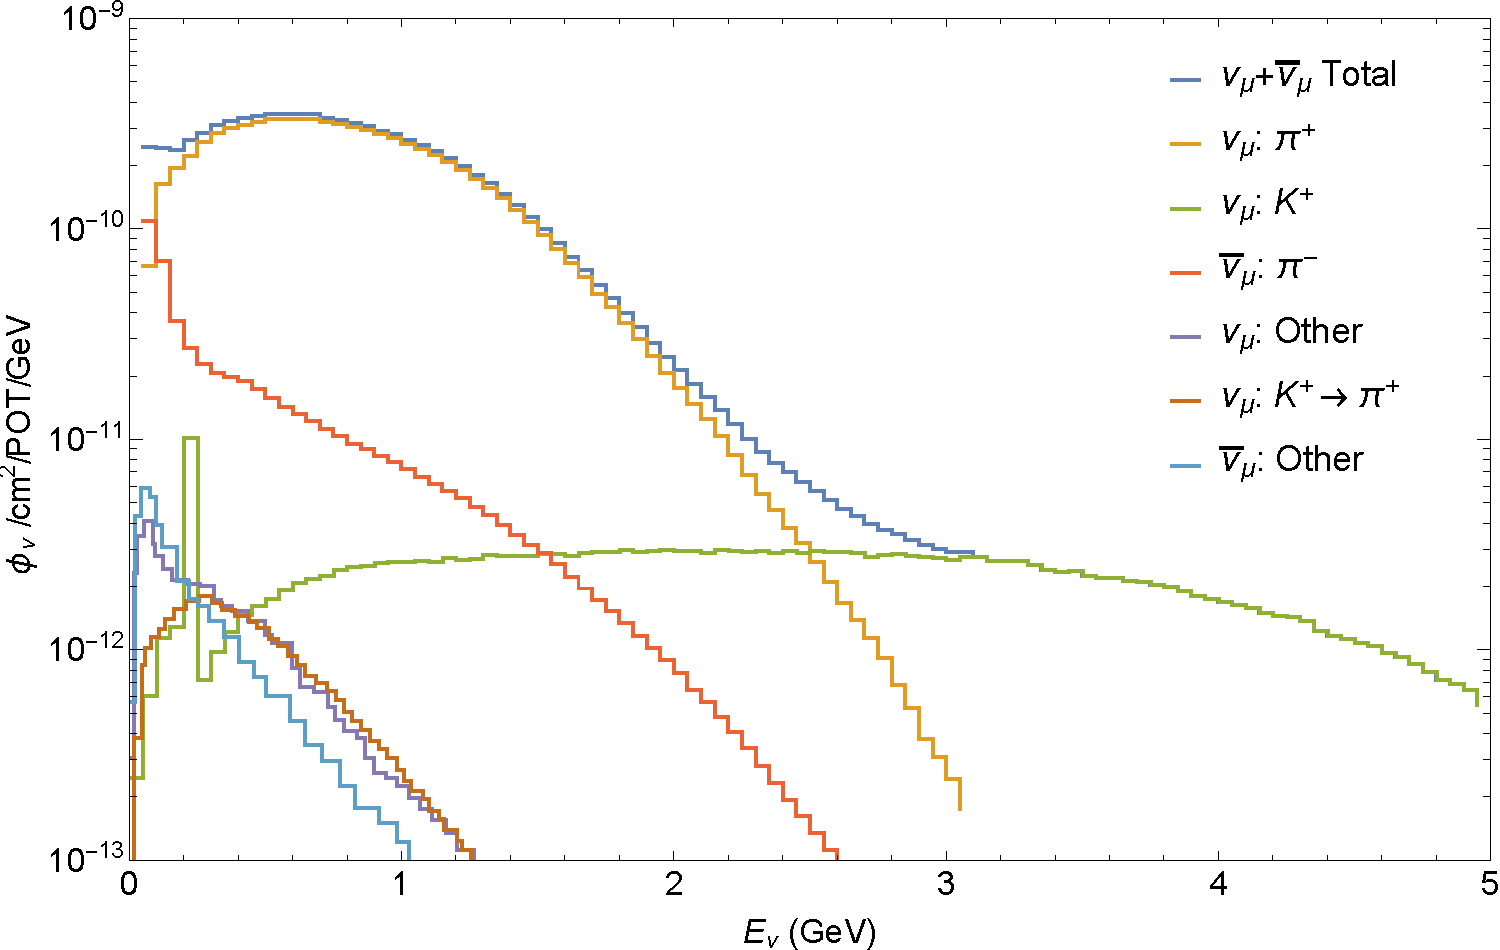
\includegraphics[width=\textwidth]{figures/microBooNE_flux.pdf} 
\end{subfigure}%
~
\begin{subfigure}[t]{0.5\textwidth}
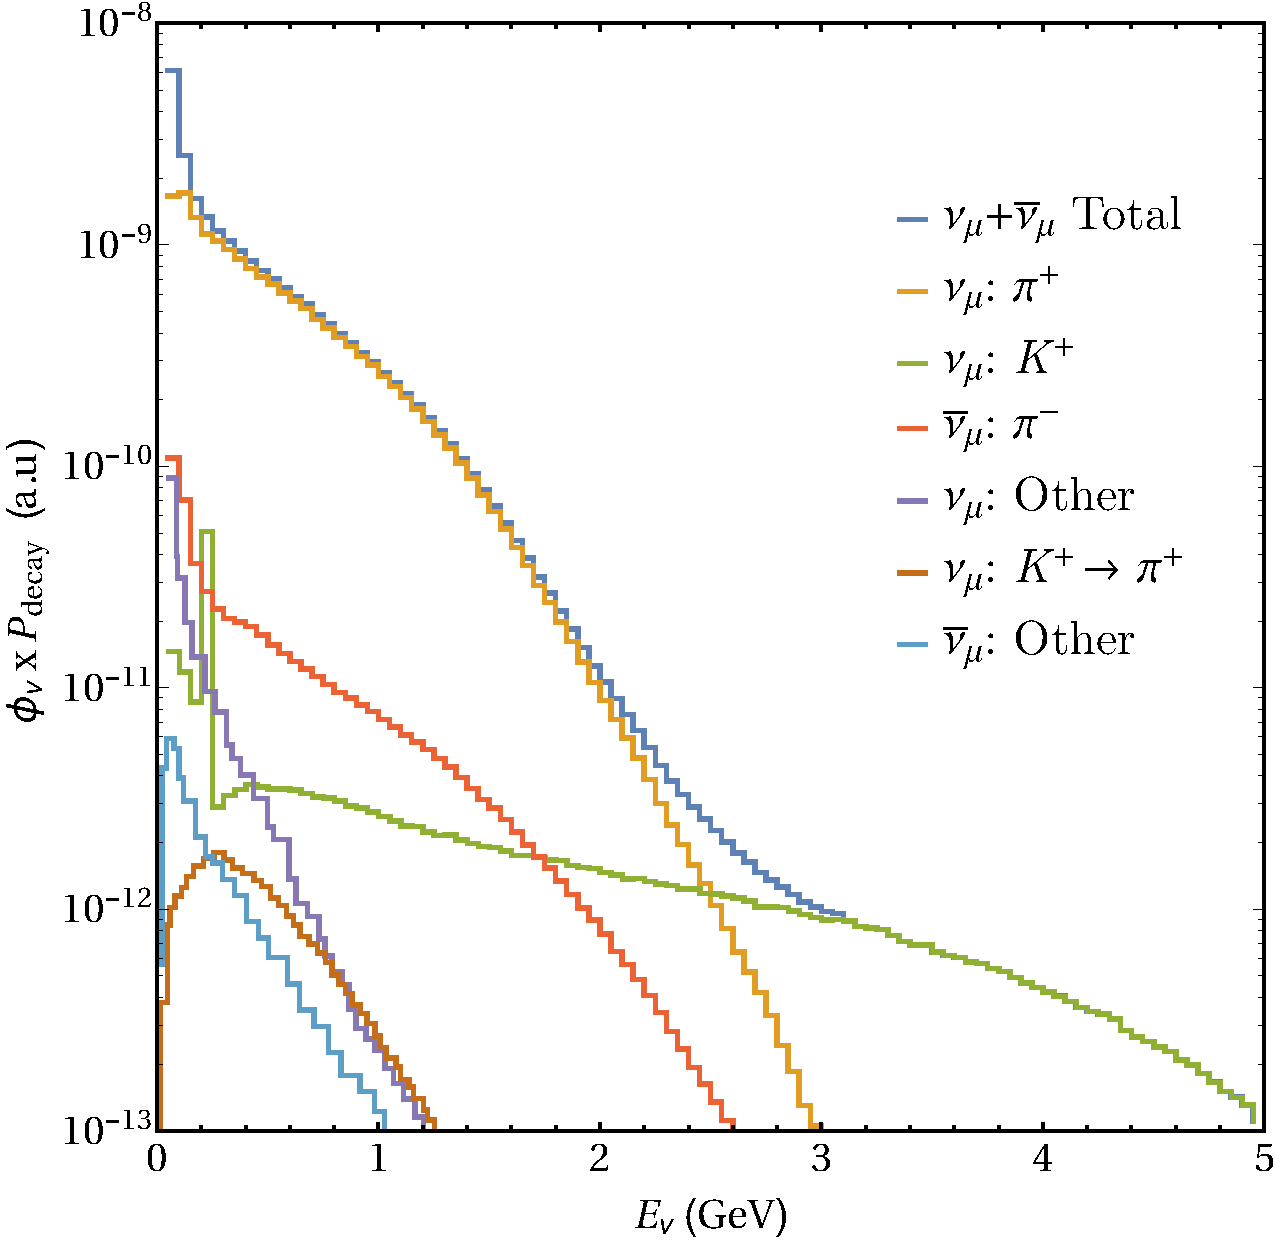
\includegraphics[width=\textwidth]{figures/microBooNE_flux_weighted.pdf}
\end{subfigure}

\caption{\label{fig:flux_plots} \emph{Left:} The composition of fluxes of $\nu_\mu$
and $\overline{\nu}_\mu$ at \muboone\ with horn in positive polarity (neutrino
mode). ``Other'' refers to contributions primarily from meson decay chains
initiated by meson-nucleus interactions.\emph{ Right:} Fluxes weighted by the
probability to decay inside \muboone, for a sample 25 MeV sterile neutrino with equal
$|U_{e4}|^2 = |U_{\mu 4}|^2$, and the horn in neutrino-mode. Requiring that the
sterile neutrino decays inside the detector has the effect of vastly increasing the importance of lower
energy bins, where traditionally cross-section induced background effects are
small.}

\end{figure}


As we are exploring a large parameter space, often this expression takes a
simplified form depending on the size of $\Gamma_\text{T}\lambda/\gamma\beta$:
%
\begin{align} 
%
\Gamma_\text{T}\lambda \ll 1\qquad&\qquad P_\text{D} \approx
e^{-\frac{\Gamma_\text{T}L}{\gamma\beta}}\frac{\Gamma_\text{c}\lambda}{\gamma\beta}
+ \mathcal{O}\left(\Gamma_\text{T}^2\lambda^2\right),\label{eq:prob_dec1}\\
%
\Gamma_\text{T}\lambda \gg 1\qquad&\qquad P_\text{D} \approx
e^{-\frac{\Gamma_\text{T}L}{\gamma\beta}}\frac{\Gamma_\text{c}}{\Gamma_\text{T}}
+ \mathcal{O}\left(\frac{1}{\Gamma_\text{T}\lambda}\right),
\label{eq:prob_dec2}
%
\end{align}
%
where the rate for slowly decaying particles can be seen to grow with detector
size until a width of $\lambda\sim\gamma\beta\Gamma_\text{T}^{-1}$.
\newtext{PB}{For detectors longer than this scale, the event rate becomes
independent of detector size, as most sterile neutrinos decay within a few
decay lengths.} 

The spectral flux of sterile neutrinos impinging on a SBN detector,
$\mathrm{d}\phi/\mathrm{d}E$, is estimated as described in \refsec{sec:prod}.
Of crucial importance to this is accurate knowledge of active neutrino fluxes
at all three SBN detectors. These are calculated from published MiniBooNE
fluxes \cite{AguilarArevalo:2008yp}, after scaling by appropriate $1/r^2$
baseline dependence, \eg\ $(470/540)^2 \approx 1.3$ at \muboone. This is
similarly scaled by $1/r^2$ for ICARUS at 600m, however, an additional energy
dependent flux modifier is applied for SBND at 110m to account for the softer
energy spectrum due to the proximity of the detector to the production target
\cite{Antonello:2015lea}. We consider sources of neutrinos that are relevant
including wrong sign neutrinos, smaller sub-dominant $K^+\rightarrow
\pi^+\rightarrow \nu_\alpha$ as well as other contributions, predominately from
meson decay chains initiated by meson-nucleus interactions. The neutrino
spectrum at \muboone\ is shown below in \reffig{fig:flux_plots}. As the
probability for any given sterile neutrins to subsequently decay inside a detector
scales as $1/|P_{\ster}|$ the fluxes of active neutrinos at low
energy are of particular importance, in stark contrast to standard neutrino
interaction cross sections, which scale as $E_\nu$. 
%
This means the effective spectrum of \emph{decaying} particles is heavily biased
towards lower energies, this can be seen in the right panel of
\reffig{fig:flux_plots}.
%
This low-energy bias exaggerates the kinematic differences between our
decay-in-flight signal and the dominant background events. 

Finally, the function $W_\text{c}(E)$ is a weighting factor which accounts for
all effects which reduce the number of events in the sample: for example,
analysis cuts or detector performance effects. 
%
To compute these factors, we run a Monte Carlo simulation of the decays for a
large number of sample events with a given energy. Each sterile neutrino event is
associated with a decay of type $\text{c}$. We then apply experimental analysis
cuts to the decays based on our assumptions about the detector's capabilities
and backgrounds, to produce a spectrum representing the final event sample when
considering events in the bucket timing window (See \refapp{app:bg} for details
of the background analysis). The percentage of accepted events defines the
weight factor for that energy. In this manner the full spectral shape of the signal is
included in the total rate analysis. As a consistency check of our methodology, we
also reproduce in \refapp{sec:ps191} some of the published bounds of PS-191. 

\subsection{\label{sec:backgroundestimate}Background reduction}

In order to estimate the impact of potential backgrounds we performed a
Monte-Carlo analysis using the neutrino event generator GENIE
\cite{Andreopoulos:2009rq}. This provides generator level information
about the kinematics of the beam-driven backgrounds, with rates normalised off
expected NC and CC inclusive values as published in the SBN proposal. Energy
and angular smearing is then implemented to allow for approximate estimates of
the effects of detector performance to the level necessary for this analysis,
without the need for a full GEANT detector simulation. Energies are smeared
according to a Gaussian distribution around their true MC energies, with a
relative variance $\sigma_E/E = \xi/ \sqrt(E) $, where $\xi$ is a detector
dependent resolution.  For this study we take the energy resolution for EM
showers, muons and protons to be 15\%, 6\% and a conservative 15\%
respectively, alongside an angular resolution in LAr of $1.73^{\circ}$
\cite{Antonello:2015lea}. 

\begin{figure}[t]
\center
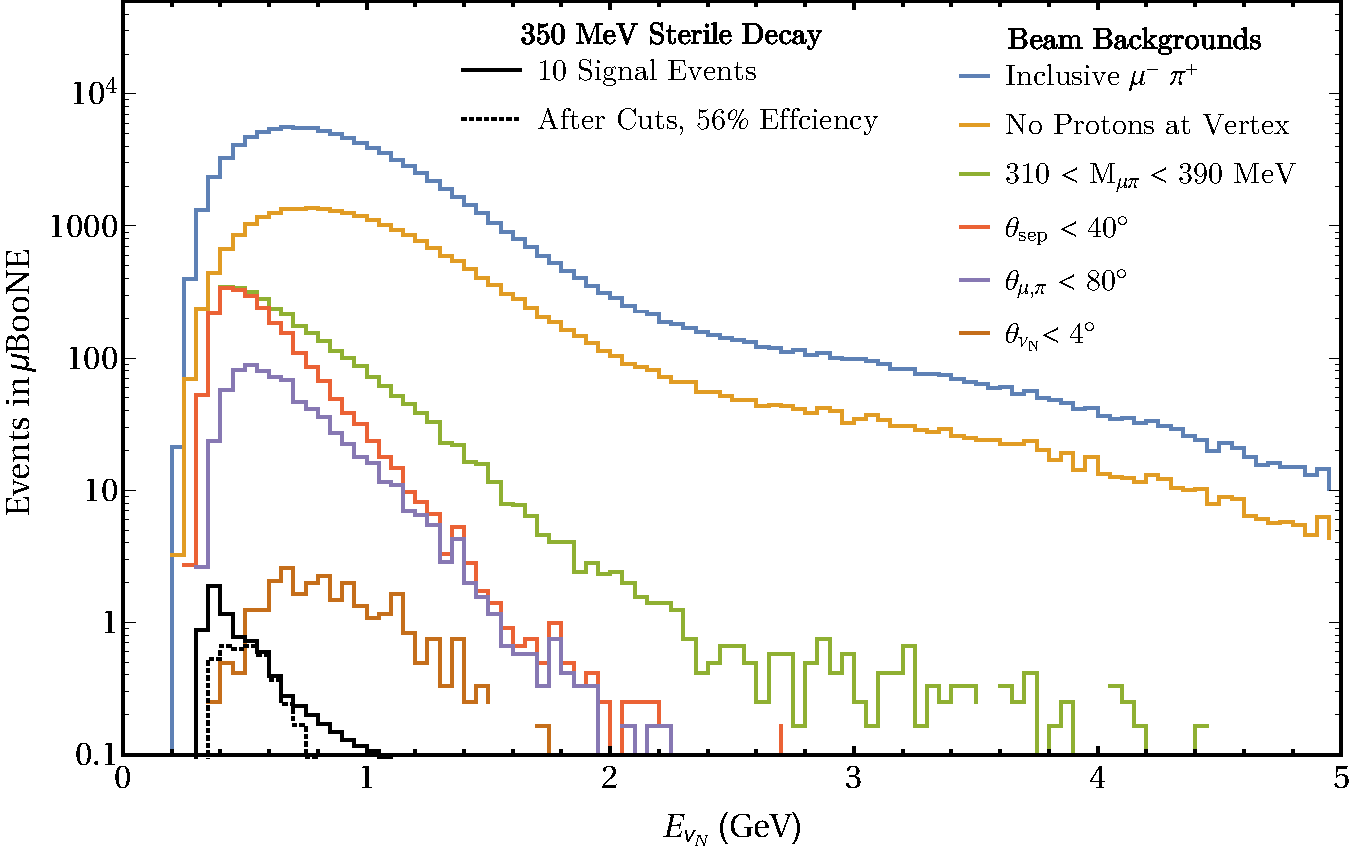
\includegraphics[width=0.6\textwidth,clip,trim=0 0 0 0]{figures/mu_pi_cutflow.pdf}

\caption{\label{fig:mu_pi_cutflow} Reconstructed sterile neutrino energy spectra for
CC$\nu_\mu$ backgrounds in comparison to a 350 MeV decaying sterile neutrino at
\muboone, normalised to 10 signal events. Total expected background of 98,013
events is reduced to $\approx$ 27 by successive kinematic cuts (as listed in legend) which utilise
the stark differences between decay-in-flight and scattering kinematics. Further cuts on energy would allow for even greater reduction. }
\end{figure}

Of utmost importance in all studied channels is the identification of a
scattering vertex, which cleanly indicates that the process is not a
decay-in-flight event. Any hadronic activity localised at the beginning of the
lepton track is a smoking gun for a deep-inelastic or quasi-elastic
beam-related scattering event. Therefore we reject any event containing one or more
reconstructed protons or additional hadrons. For counting
this proton multiplicity we assume a detection threshold of 21 MeV on proton
kinetic energy in liquid Argon \cite{Acciarri:2014gev}, after smearing.
Background events with energies below this threshold and events that do not contain
any protons (such as events originating from coherent pion production) remain a
viable background and further rejection must come from the kinematics of the
final state particles only. The kinematics of such daughter particles
originating from decay-in-flight and backgrounds from scattering events,
however,  have strikingly different behaviour leading to strong suppression
capabilities.

As a representative example of our analysis we discuss the backgrounds
associated with the decay $\ster \rightarrow \mu^\pm \pi^\mp$, the channel with
largest expected beam related backgrounds in all SBN detectors, the dominant
component of which arises from genuine charged current $\pi \mu$ production.
This channel, and indeed $e^\pm \pi^\mp$, has a powerful discriminator in the
reconstructed invariant mass of the charged particle pair, \eg\  $M_{l^\pm
\pi^\mp}^2=m_l^2+m_{\pi^\pm}^2+ 2(E_l E_\pi - |P_l||P_\pi|\cos\theta_\text{sep})$
for $\ster\rightarrow \pi^\pm l^\mp$, which sum to that of the the parent
sterile neutrinno (within detector resolution), where as the background forms
a broad spectrum across the energies of the incoming neutrinos. On top of this strong invariant mass discriminator, these two body decays allow for reconstruction of the 
parent sterile neutrino angle with respect to the beamline which is very
close to on-axis, as opposed to the more isotropic backgrounds. We find that
approximately $95$\% of the reconstructed sterile neutrino angles from these
decays are inside a $4^\circ$ cone centred on the beamline. 

We show the effect of our cuts for this channel in \reffig{fig:mu_pi_cutflow},
which ultimately leads to a reduction in the inclusive $\mu \pi$ eventrate at
MicroBooNE (SBND) from around $10^5, (1.5\times10^6)$ to around $30 (300)$
while maintaining a signal efficiency of $56\%$. This level of background
suppression crucially relies on the angular and energy resolution of LAr
detectors, but requires no modification to the current design. 

For a parallel discussion of the backgrounds for the remaining channels see
\refapp{app:bg}.

\subsection{\label{sec:timing}Role of event timing}

\begin{figure}[t] \center \begin{subfigure}[c]{0.68\textwidth}
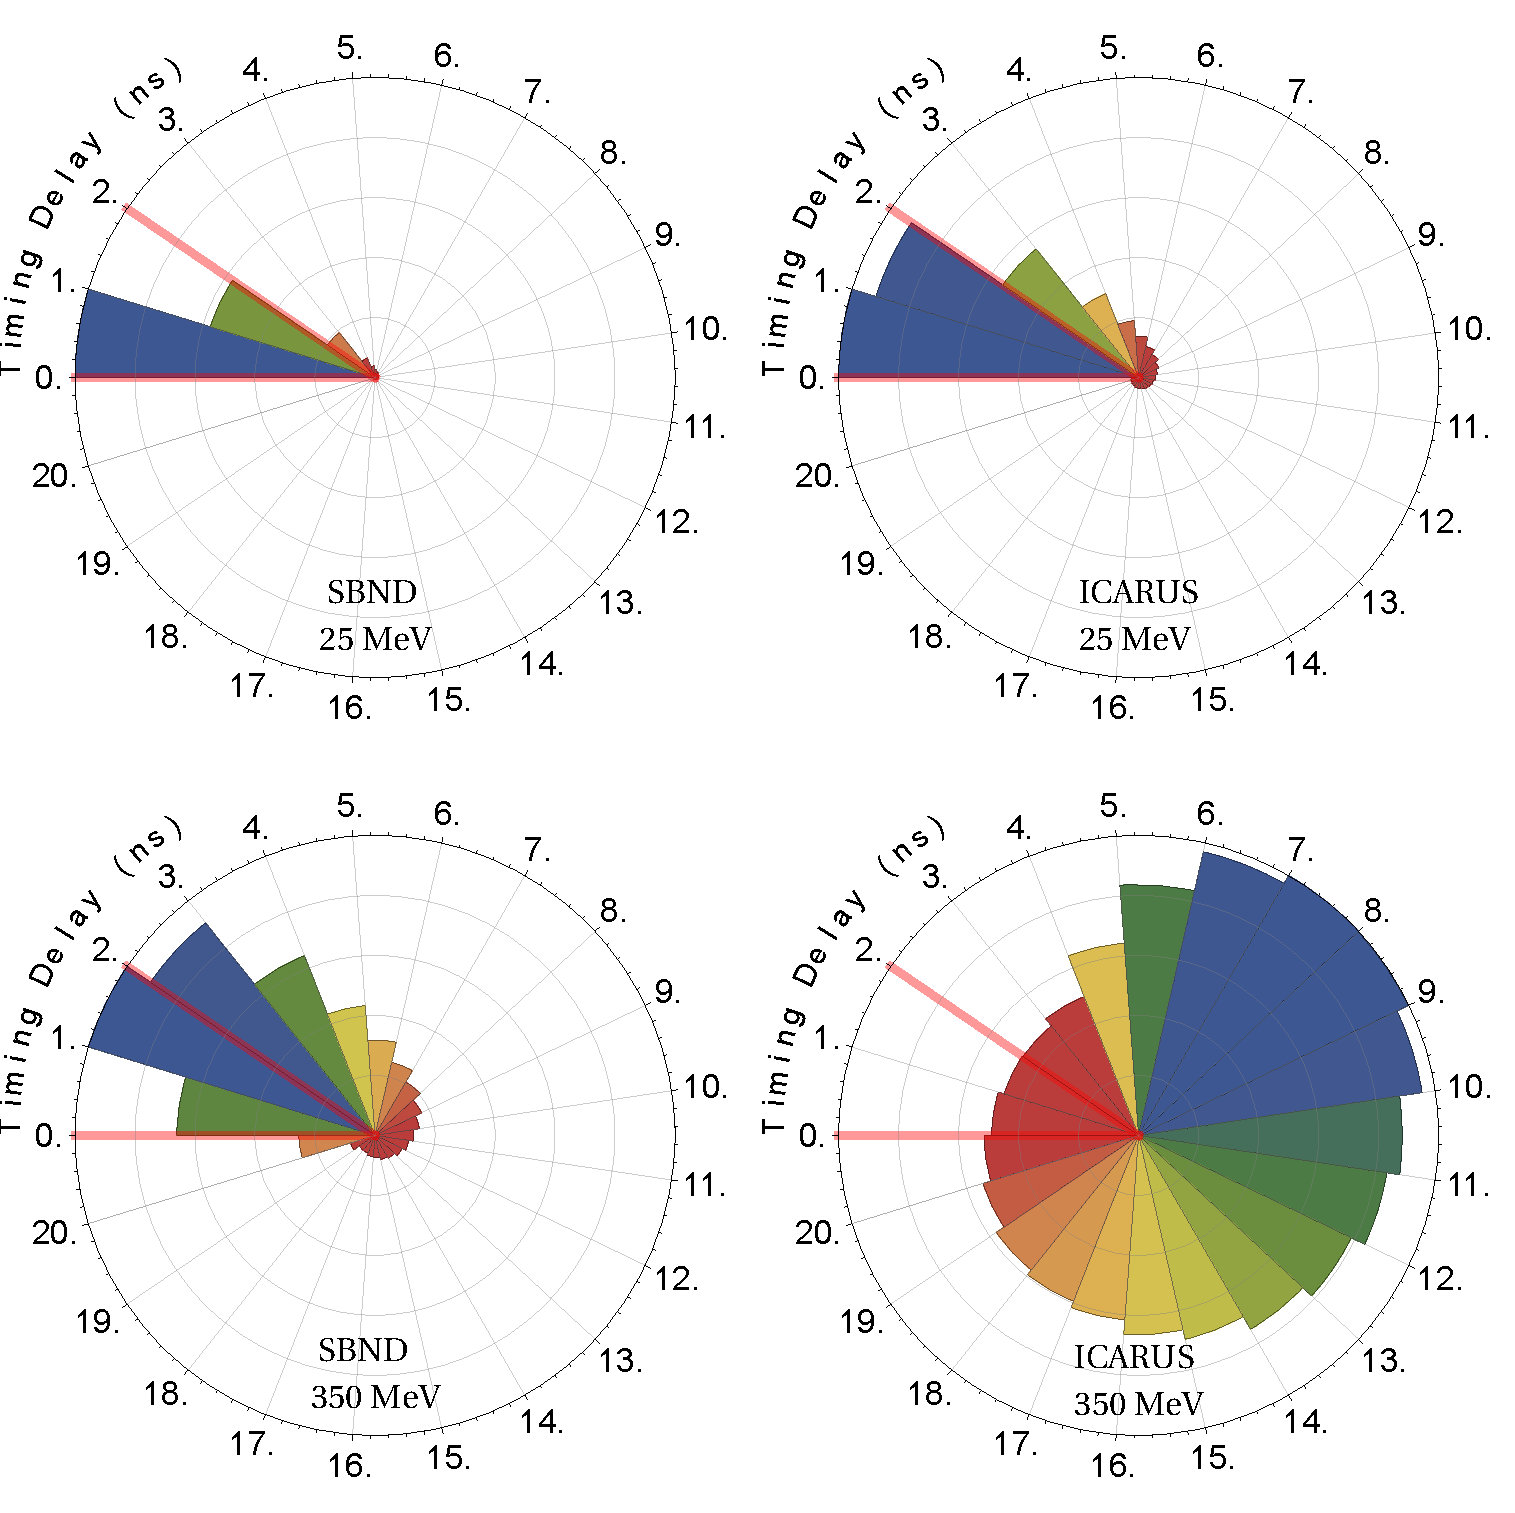
\includegraphics[width=\textwidth]{figures/timing.pdf} \end{subfigure}% ~
\begin{subfigure}[c]{0.32\textwidth}
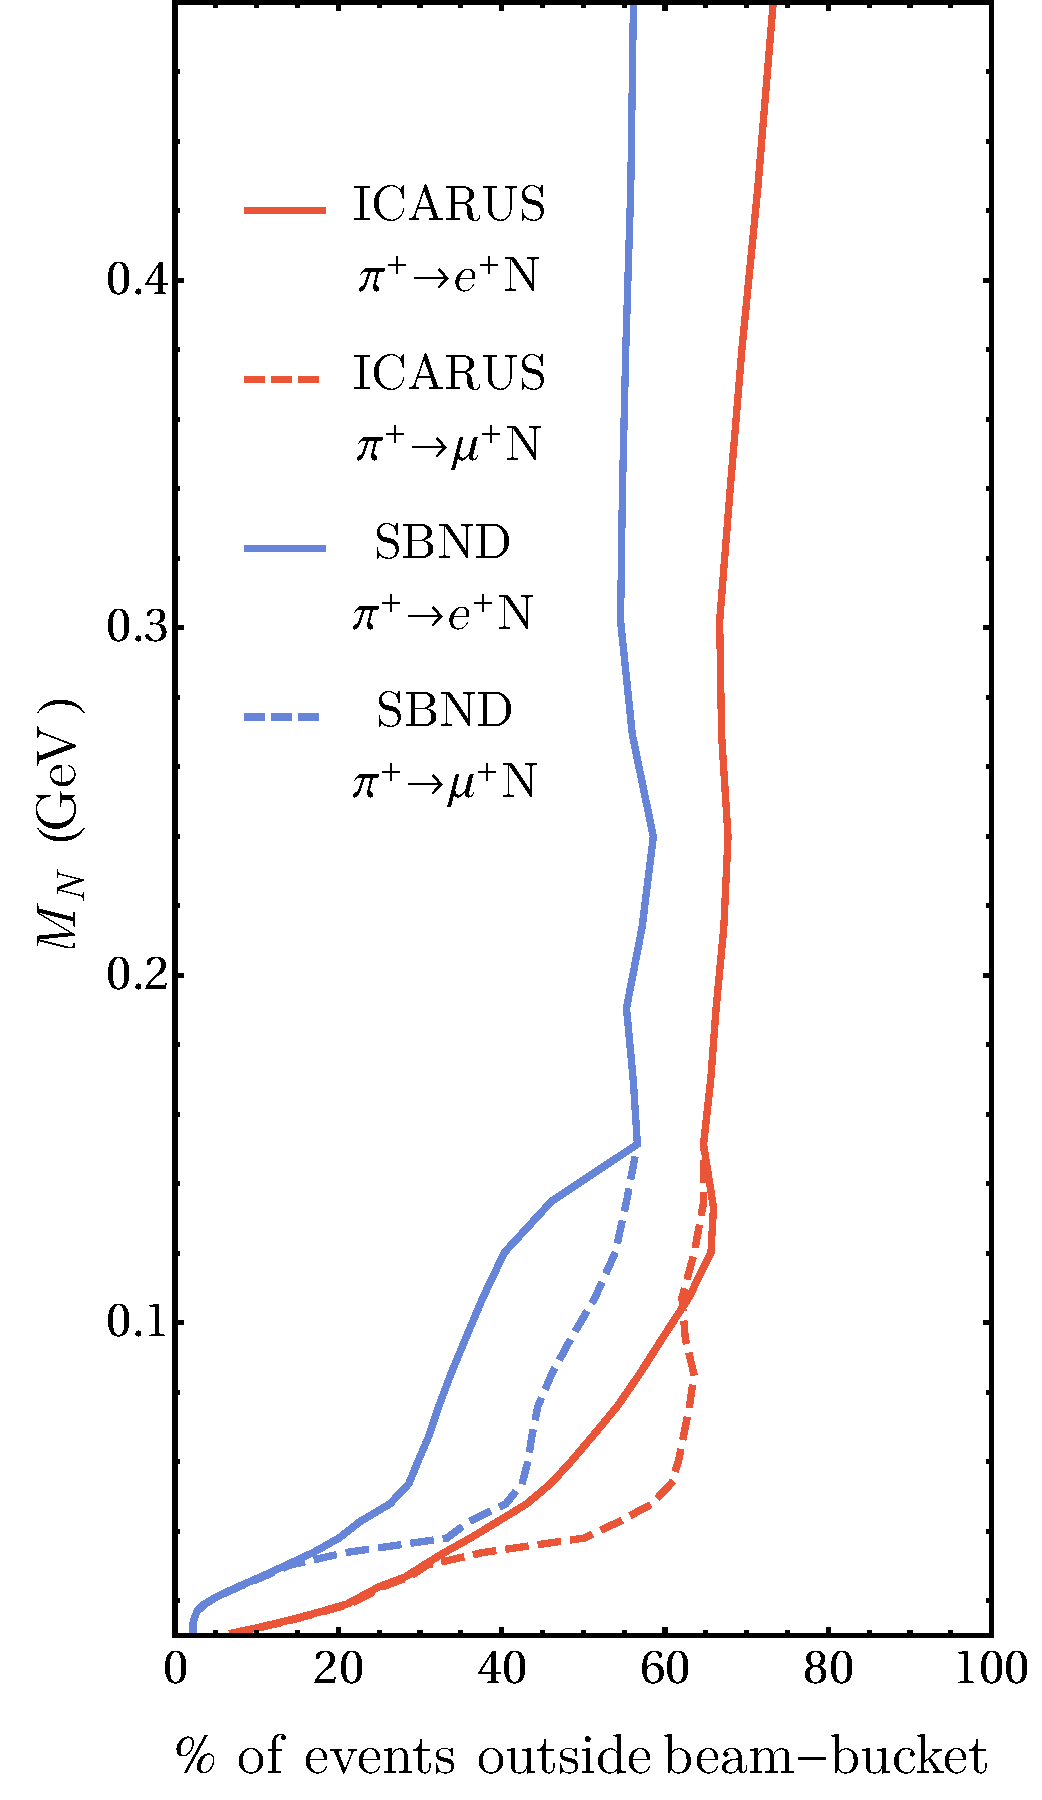
\includegraphics[width=\textwidth]{figures/line_plots_long.pdf} \end{subfigure}
\caption{\label{fig:timing} \emph{Left:} The timing delay of sterile neutrino
decays in nano-seconds for both a 25 MeV (top) and 350 MeV (bottom) sterile
neutrino at the SBND and and \icarus\ detectors (110 and 600m respectively).
The 4 ns beam bucket window is shown highlighted in red from 0 to 4 ns,
followed by an additional 17 ns gap. The timings are calculated as a difference
to the time of flight of a active neutrino, assuming the decay occurred in a
uniform sample across the 50m BNB decay pipe. A timing resolution of 1 ns is
assumed to smear the observed events. \emph{Right:} The percentage of sterile neutrino
decay events that fall into the inter-bucket region as a function of sterile neutrino
mass for SBND and ICARUS, assuming a flux derived from $U_{e4}$ ($U_{\mu 4}$)
mixing in solid (dashed) lines. Both SBND and ICARUS see a sizable fraction of
total events outside the beam bucket windows when the sterile neutrino mass exceeds
$\approx10$ MeV.  }

\end{figure}

On top of the impressive background rejection capabilities of LAr from
kinematic cuts, there is the potential for an even greater background 
suppression by considering the time of arrival of observed events. Although the 
drift time of electrons in LAr can be as large as $100$~$\mu$s, the ionisation
and excitation of Argon from the passage of a charged particle also produces
128~nm scintillation light of which there is a nano-second scale contribution
from the decay of the excited state $\text{Ar}^*_2$ \cite{Acciarri:2015hha}. LAr is
transparent to this light, and if the light detection system (LDS) employed by
the SBN detectors has a nanosecond resolution, this can allow for
precise timing to be attached to each TPC triggered event.

Light neutrinos propagate and reach the furthest detector of the SBN complex
after approximately 2 $\mu$s. In the conventional physics program of the SBN,
the timing of these events play an important role in the analysis of
backgrounds, tight timing windows are placed around the 19.2$\mu$s beam spill
to limit constant rate backgrounds such as cosmogenic events
\cite{Antonello:2015lea}. The LDS of both SBND and ICARUS, however, are
expected to be able to achieve significantly better timing resolution than
this, around $1$--$2$~ns depending on the exact technology used, which
potentially allows for the use of both bucket and spill structure in the
background analysis. The BNB consists of 81 Radio-Frequency buckets of
approximately 2~ns length, separated by 19~ns, to form the 19.2~$\mu$s spill
with a frequency of 3~Hz \cite{Antonello:2015lea}.  If this nano-second
resolution is indeed achieved, it allows for events in individual buckets to be
identified.  Such a nano-second resolution was achieved previously by the PMTs
used in MiniBooNE \cite{Antonello:2015lea}, with potential for improvement in
the next generation SBN detectors. \muboone\ is omitted from considerations of
timing as its achievable timing resolution is lower at around $10$~ns
\cite{Katori:2013wqa}.

As particles with finite rest mass, heavy sterile neutrinos will propagate at
subluminal speeds which can produce observable timing delays.  This effect
begins to become relevant when the sterile neutrinos have MeV-scale masses and
above. As the flux of decaying sterile neutrinos is inversely proportional to
its momentum after convolving with their decay probability, many of these low
energy sterile neutrinos are travelling at sufficiently slower speeds than their light
counterparts to be distinguishable. Shown on the right of \reffig{fig:timing}
is the fraction of events that are expected to fall outside the  bucket window
in both SBND and ICARUS. For the purposes of this study we define the
beam-correlated window to be a $6$~ns period, $2$~ns each side of the $2$~ns
beam bucket.
%
Delayed events can be observed in any subsequent window which leads to a
21-fold degeneracy in their reconstructed arrival time. In this
section, we consider only the timing of events relative to the
bucket window\footnote{Absolute
arrival times could in principle lift this degeneracy, although this would
require good synchronisation with the beam spill. Alternatively, the relative
timing between signal and beam-related backgrounds could be used. However, we
do not consider these options further.}, a structure which repeats every 21 ns. This lends a cyclical nature to the
timing information, with a distinctive structure at the different detector
sites for larger masses. Some illustrative timing distributions are shown on
the left of \reffig{fig:timing} for a $25$ and $350$ MeV sterile neutrino.
%

We find a significant proportion of sterile neutrino events distributed throughout the
inter-bucket region. Events which fall into the beam-bucket timing window have
to be analysed on top of all known beam-related backgrounds, but events in the
inter-bucket window have significantly reduced beam-correlated backgrounds. 
%
For larger masses, we have shown that the majority of events fall into these
regions, and this may allow for a low background search strategy for decaying
sterile neutrinos. Instead of beam-correlated backgrounds, the constant rate backgrounds
will limit the sensitivity for this analysis. Understanding these backgrounds
in detail is beyond the scope of this work; however, we expect the strongly
forward kinematics, combined with \emph{in situ} beam-off measurements will allow
for a very low backgrounds to be obtained.

%Cosmogenic backgrounds are not expected to play a major role, as the
%combination of fiducial veto, trajectory and particle composition can be well
%understood from in-situ inter-spill and beam-off measurements. In the main
%$\nu_e$ analysis, the single electron signal is easily mimicked by cosmic
%$\gamma$ backgrounds but despite this rates of only  146 (88,164) events in
%SBND (\muboone, ICARUS) after fiducial and $dE/dx$ cuts
%\cite{Antonello:2015lea}, are expected. As the decay in flight signatures are
%much more complicated, e.g $\pi \mu$ originating at a single point coming
%directly along the beamline, we believe cosmogenic backgrounds will not be a
%problem. A detailed analysis of the potential non-beam related backgrounds
%would be necessary but is beyond the scope of this work.

In the following sections, timing information will inform our work in three
ways. First we will compute SBN's sensitivity to decaying sterile neutrinos assuming the
full backgrounds, reduced only by the cut-based analysis discussed previously.
This is a proven sensitivity, applicable for all sterile neutrino masses and detectors
and is independent of the attainable timing resolution. Secondly, we compute a
backgroundless sensitivity. This can be seen as either the result of improved
analysis techniques, or as the inclusion of timing information at SBND and
ICARUS for the largest masses. Finally, in \refsec{sec:timing}, we will study
the use of the timing information itself to constrain the underlying model of
decaying sterile neutrinos.

%
%The implication of the timing effects is that our discussion of backgrounds is
%twofold: for low mass steriles, or any mass at \muboone\ due to its worse
%timing resolution, we must consider all beam-related backgrounds as potential
%backgrounds. For larger masses at SBND and ICARUS, we instead reduce the number
%of signal events by the appropriate fraction that lies in the bucket window and
%assume that the beam-related backgrounds are removed. 
%

\subsection{\label{sec:eventspectra}Event spectra}

\begin{figure}[t]
\begin{subfigure}[t]{\textwidth}
	\center
	%
	\large

	\resizebox{\columnwidth}{!}{% GNUPLOT: LaTeX picture with Postscript
\begingroup
  \fontfamily{ptm}%
  \selectfont
  \makeatletter
  \providecommand\color[2][]{%
    \GenericError{(gnuplot) \space\space\space\@spaces}{%
      Package color not loaded in conjunction with
      terminal option `colourtext'%
    }{See the gnuplot documentation for explanation.%
    }{Either use 'blacktext' in gnuplot or load the package
      color.sty in LaTeX.}%
    \renewcommand\color[2][]{}%
  }%
  \providecommand\includegraphics[2][]{%
    \GenericError{(gnuplot) \space\space\space\@spaces}{%
      Package graphicx or graphics not loaded%
    }{See the gnuplot documentation for explanation.%
    }{The gnuplot epslatex terminal needs graphicx.sty or graphics.sty.}%
    \renewcommand\includegraphics[2][]{}%
  }%
  \providecommand\rotatebox[2]{#2}%
  \@ifundefined{ifGPcolor}{%
    \newif\ifGPcolor
    \GPcolortrue
  }{}%
  \@ifundefined{ifGPblacktext}{%
    \newif\ifGPblacktext
    \GPblacktexttrue
  }{}%
  % define a \g@addto@macro without @ in the name:
  \let\gplgaddtomacro\g@addto@macro
  % define empty templates for all commands taking text:
  \gdef\gplbacktext{}%
  \gdef\gplfronttext{}%
  \makeatother
  \ifGPblacktext
    % no textcolor at all
    \def\colorrgb#1{}%
    \def\colorgray#1{}%
  \else
    % gray or color?
    \ifGPcolor
      \def\colorrgb#1{\color[rgb]{#1}}%
      \def\colorgray#1{\color[gray]{#1}}%
      \expandafter\def\csname LTw\endcsname{\color{white}}%
      \expandafter\def\csname LTb\endcsname{\color{black}}%
      \expandafter\def\csname LTa\endcsname{\color{black}}%
      \expandafter\def\csname LT0\endcsname{\color[rgb]{1,0,0}}%
      \expandafter\def\csname LT1\endcsname{\color[rgb]{0,1,0}}%
      \expandafter\def\csname LT2\endcsname{\color[rgb]{0,0,1}}%
      \expandafter\def\csname LT3\endcsname{\color[rgb]{1,0,1}}%
      \expandafter\def\csname LT4\endcsname{\color[rgb]{0,1,1}}%
      \expandafter\def\csname LT5\endcsname{\color[rgb]{1,1,0}}%
      \expandafter\def\csname LT6\endcsname{\color[rgb]{0,0,0}}%
      \expandafter\def\csname LT7\endcsname{\color[rgb]{1,0.3,0}}%
      \expandafter\def\csname LT8\endcsname{\color[rgb]{0.5,0.5,0.5}}%
    \else
      % gray
      \def\colorrgb#1{\color{black}}%
      \def\colorgray#1{\color[gray]{#1}}%
      \expandafter\def\csname LTw\endcsname{\color{white}}%
      \expandafter\def\csname LTb\endcsname{\color{black}}%
      \expandafter\def\csname LTa\endcsname{\color{black}}%
      \expandafter\def\csname LT0\endcsname{\color{black}}%
      \expandafter\def\csname LT1\endcsname{\color{black}}%
      \expandafter\def\csname LT2\endcsname{\color{black}}%
      \expandafter\def\csname LT3\endcsname{\color{black}}%
      \expandafter\def\csname LT4\endcsname{\color{black}}%
      \expandafter\def\csname LT5\endcsname{\color{black}}%
      \expandafter\def\csname LT6\endcsname{\color{black}}%
      \expandafter\def\csname LT7\endcsname{\color{black}}%
      \expandafter\def\csname LT8\endcsname{\color{black}}%
    \fi
  \fi
  \setlength{\unitlength}{0.0500bp}%
  \begin{picture}(11320.00,3400.00)%
    \gplgaddtomacro\gplbacktext{%
      \colorrgb{0.50,0.50,0.50}%
      \put(918,680){\makebox(0,0)[r]{\strut{} 0}}%
      \colorrgb{0.50,0.50,0.50}%
      \put(918,1045){\makebox(0,0)[r]{\strut{} 0.1}}%
      \colorrgb{0.50,0.50,0.50}%
      \put(918,1411){\makebox(0,0)[r]{\strut{} 0.2}}%
      \colorrgb{0.50,0.50,0.50}%
      \put(918,1776){\makebox(0,0)[r]{\strut{} 0.3}}%
      \colorrgb{0.50,0.50,0.50}%
      \put(918,2141){\makebox(0,0)[r]{\strut{} 0.4}}%
      \colorrgb{0.50,0.50,0.50}%
      \put(918,2507){\makebox(0,0)[r]{\strut{} 0.5}}%
      \colorrgb{0.50,0.50,0.50}%
      \put(918,2872){\makebox(0,0)[r]{\strut{} 0.6}}%
      \colorrgb{0.50,0.50,0.50}%
      \put(1020,494){\makebox(0,0){\strut{} 0}}%
      \colorrgb{0.50,0.50,0.50}%
      \put(1897,494){\makebox(0,0){\strut{} 0.2}}%
      \colorrgb{0.50,0.50,0.50}%
      \put(2774,494){\makebox(0,0){\strut{} 0.4}}%
      \colorrgb{0.50,0.50,0.50}%
      \put(3650,494){\makebox(0,0){\strut{} 0.6}}%
      \colorrgb{0.50,0.50,0.50}%
      \put(4527,494){\makebox(0,0){\strut{} 0.8}}%
      \colorrgb{0.50,0.50,0.50}%
      \put(5404,494){\makebox(0,0){\strut{} 1}}%
      \csname LTb\endcsname%
      \put(315,1776){\rotatebox{-270}{\makebox(0,0){\strut{}Frequency}}}%
      \csname LTb\endcsname%
      \put(5589,1776){\rotatebox{-270}{\makebox(0,0){\strut{}}}}%
      \csname LTb\endcsname%
      \put(3212,215){\makebox(0,0){\strut{}E (GeV)}}%
      \put(3212,2779){\makebox(0,0){\strut{}}}%
      \csname LTb\endcsname%
      \put(3212,2778){\makebox(0,0){\strut{}}}%
      \put(408,178){\makebox(0,0)[l]{\strut{}}}%
      \put(3650,1776){\makebox(0,0)[l]{\strut{}decay to $\nu e^+ e^-$}}%
    }%
    \gplgaddtomacro\gplfronttext{%
      \csname LTb\endcsname%
      \put(4616,2612){\makebox(0,0)[r]{\strut{}100 MeV}}%
      \csname LTb\endcsname%
      \put(4616,2426){\makebox(0,0)[r]{\strut{}200 MeV}}%
      \csname LTb\endcsname%
      \put(4616,2240){\makebox(0,0)[r]{\strut{}350 MeV}}%
    }%
    \gplgaddtomacro\gplbacktext{%
      \colorrgb{0.50,0.50,0.50}%
      \put(6578,680){\makebox(0,0)[r]{\strut{} 0}}%
      \colorrgb{0.50,0.50,0.50}%
      \put(6578,1045){\makebox(0,0)[r]{\strut{} 0.05}}%
      \colorrgb{0.50,0.50,0.50}%
      \put(6578,1411){\makebox(0,0)[r]{\strut{} 0.1}}%
      \colorrgb{0.50,0.50,0.50}%
      \put(6578,1776){\makebox(0,0)[r]{\strut{} 0.15}}%
      \colorrgb{0.50,0.50,0.50}%
      \put(6578,2141){\makebox(0,0)[r]{\strut{} 0.2}}%
      \colorrgb{0.50,0.50,0.50}%
      \put(6578,2507){\makebox(0,0)[r]{\strut{} 0.25}}%
      \colorrgb{0.50,0.50,0.50}%
      \put(6578,2872){\makebox(0,0)[r]{\strut{} 0.3}}%
      \colorrgb{0.50,0.50,0.50}%
      \put(6680,494){\makebox(0,0){\strut{} 0}}%
      \colorrgb{0.50,0.50,0.50}%
      \put(7557,494){\makebox(0,0){\strut{} 0.2}}%
      \colorrgb{0.50,0.50,0.50}%
      \put(8434,494){\makebox(0,0){\strut{} 0.4}}%
      \colorrgb{0.50,0.50,0.50}%
      \put(9310,494){\makebox(0,0){\strut{} 0.6}}%
      \colorrgb{0.50,0.50,0.50}%
      \put(10187,494){\makebox(0,0){\strut{} 0.8}}%
      \colorrgb{0.50,0.50,0.50}%
      \put(11064,494){\makebox(0,0){\strut{} 1}}%
      \csname LTb\endcsname%
      \put(5873,1776){\rotatebox{-270}{\makebox(0,0){\strut{}Frequency}}}%
      \csname LTb\endcsname%
      \put(11249,1776){\rotatebox{-270}{\makebox(0,0){\strut{}}}}%
      \csname LTb\endcsname%
      \put(8872,215){\makebox(0,0){\strut{}E (GeV)}}%
      \put(8872,2779){\makebox(0,0){\strut{}}}%
      \csname LTb\endcsname%
      \put(8872,2778){\makebox(0,0){\strut{}}}%
      \put(5966,178){\makebox(0,0)[l]{\strut{}}}%
      \put(9310,1776){\makebox(0,0)[l]{\strut{}decay to $\nu e^+ e^-$}}%
    }%
    \gplgaddtomacro\gplfronttext{%
      \csname LTb\endcsname%
      \put(10276,2612){\makebox(0,0)[r]{\strut{}100 MeV}}%
      \csname LTb\endcsname%
      \put(10276,2426){\makebox(0,0)[r]{\strut{}200 MeV}}%
      \csname LTb\endcsname%
      \put(10276,2240){\makebox(0,0)[r]{\strut{}350 MeV}}%
    }%
    \gplbacktext
    \put(0,0){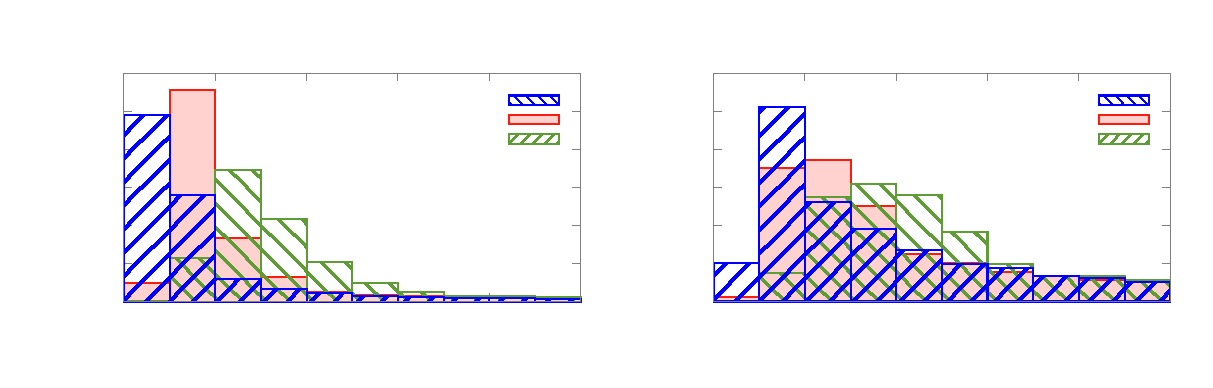
\includegraphics{figures/spectrum}}%
    \gplfronttext
  \end{picture}%
\endgroup
}\\

	%
	%
\end{subfigure}\\

\begin{subfigure}[c]{\textwidth}
	\center
	\large
	\resizebox{0.7\columnwidth}{!}{% GNUPLOT: LaTeX picture with Postscript
\begingroup
  \fontfamily{ptm}%
  \selectfont
  \makeatletter
  \providecommand\color[2][]{%
    \GenericError{(gnuplot) \space\space\space\@spaces}{%
      Package color not loaded in conjunction with
      terminal option `colourtext'%
    }{See the gnuplot documentation for explanation.%
    }{Either use 'blacktext' in gnuplot or load the package
      color.sty in LaTeX.}%
    \renewcommand\color[2][]{}%
  }%
  \providecommand\includegraphics[2][]{%
    \GenericError{(gnuplot) \space\space\space\@spaces}{%
      Package graphicx or graphics not loaded%
    }{See the gnuplot documentation for explanation.%
    }{The gnuplot epslatex terminal needs graphicx.sty or graphics.sty.}%
    \renewcommand\includegraphics[2][]{}%
  }%
  \providecommand\rotatebox[2]{#2}%
  \@ifundefined{ifGPcolor}{%
    \newif\ifGPcolor
    \GPcolortrue
  }{}%
  \@ifundefined{ifGPblacktext}{%
    \newif\ifGPblacktext
    \GPblacktexttrue
  }{}%
  % define a \g@addto@macro without @ in the name:
  \let\gplgaddtomacro\g@addto@macro
  % define empty templates for all commands taking text:
  \gdef\gplbacktext{}%
  \gdef\gplfronttext{}%
  \makeatother
  \ifGPblacktext
    % no textcolor at all
    \def\colorrgb#1{}%
    \def\colorgray#1{}%
  \else
    % gray or color?
    \ifGPcolor
      \def\colorrgb#1{\color[rgb]{#1}}%
      \def\colorgray#1{\color[gray]{#1}}%
      \expandafter\def\csname LTw\endcsname{\color{white}}%
      \expandafter\def\csname LTb\endcsname{\color{black}}%
      \expandafter\def\csname LTa\endcsname{\color{black}}%
      \expandafter\def\csname LT0\endcsname{\color[rgb]{1,0,0}}%
      \expandafter\def\csname LT1\endcsname{\color[rgb]{0,1,0}}%
      \expandafter\def\csname LT2\endcsname{\color[rgb]{0,0,1}}%
      \expandafter\def\csname LT3\endcsname{\color[rgb]{1,0,1}}%
      \expandafter\def\csname LT4\endcsname{\color[rgb]{0,1,1}}%
      \expandafter\def\csname LT5\endcsname{\color[rgb]{1,1,0}}%
      \expandafter\def\csname LT6\endcsname{\color[rgb]{0,0,0}}%
      \expandafter\def\csname LT7\endcsname{\color[rgb]{1,0.3,0}}%
      \expandafter\def\csname LT8\endcsname{\color[rgb]{0.5,0.5,0.5}}%
    \else
      % gray
      \def\colorrgb#1{\color{black}}%
      \def\colorgray#1{\color[gray]{#1}}%
      \expandafter\def\csname LTw\endcsname{\color{white}}%
      \expandafter\def\csname LTb\endcsname{\color{black}}%
      \expandafter\def\csname LTa\endcsname{\color{black}}%
      \expandafter\def\csname LT0\endcsname{\color{black}}%
      \expandafter\def\csname LT1\endcsname{\color{black}}%
      \expandafter\def\csname LT2\endcsname{\color{black}}%
      \expandafter\def\csname LT3\endcsname{\color{black}}%
      \expandafter\def\csname LT4\endcsname{\color{black}}%
      \expandafter\def\csname LT5\endcsname{\color{black}}%
      \expandafter\def\csname LT6\endcsname{\color{black}}%
      \expandafter\def\csname LT7\endcsname{\color{black}}%
      \expandafter\def\csname LT8\endcsname{\color{black}}%
    \fi
  \fi
  \setlength{\unitlength}{0.0500bp}%
  \begin{picture}(9060.00,4520.00)%
    \gplgaddtomacro\gplbacktext{%
      \csname LTb\endcsname%
      \put(533,2455){\rotatebox{-270}{\makebox(0,0){\strut{}Frequency}}}%
      \csname LTb\endcsname%
      \put(8456,2455){\rotatebox{-270}{\makebox(0,0){\strut{}}}}%
      \csname LTb\endcsname%
      \put(4550,130){\makebox(0,0){\strut{}$\cos\theta$}}%
      \put(4550,4222){\makebox(0,0){\strut{}}}%
      \csname LTb\endcsname%
      \put(4550,4221){\makebox(0,0){\strut{}}}%
      \put(626,93){\makebox(0,0)[l]{\strut{}}}%
      \put(1425,3105){\makebox(0,0)[l]{\strut{}$m_N = 100$ MeV}}%
    }%
    \gplgaddtomacro\gplfronttext{%
      \csname LTb\endcsname%
      \put(2934,3856){\makebox(0,0)[r]{\strut{}true decay rate}}%
      \csname LTb\endcsname%
      \put(2934,3540){\makebox(0,0)[r]{\strut{}flat decay rate}}%
      \colorrgb{0.50,0.50,0.50}%
      \put(728,1525){\makebox(0,0)[r]{\strut{}}}%
      \colorrgb{0.50,0.50,0.50}%
      \put(728,2455){\makebox(0,0)[r]{\strut{}}}%
      \colorrgb{0.50,0.50,0.50}%
      \put(728,3385){\makebox(0,0)[r]{\strut{}}}%
      \colorrgb{0.50,0.50,0.50}%
      \put(728,4315){\makebox(0,0)[r]{\strut{}}}%
      \colorrgb{0.50,0.50,0.50}%
      \put(830,409){\makebox(0,0){\strut{} 0}}%
      \colorrgb{0.50,0.50,0.50}%
      \put(1574,409){\makebox(0,0){\strut{} 0.1}}%
      \colorrgb{0.50,0.50,0.50}%
      \put(2318,409){\makebox(0,0){\strut{} 0.2}}%
      \colorrgb{0.50,0.50,0.50}%
      \put(3062,409){\makebox(0,0){\strut{} 0.3}}%
      \colorrgb{0.50,0.50,0.50}%
      \put(3806,409){\makebox(0,0){\strut{} 0.4}}%
      \colorrgb{0.50,0.50,0.50}%
      \put(4551,409){\makebox(0,0){\strut{} 0.5}}%
      \colorrgb{0.50,0.50,0.50}%
      \put(5295,409){\makebox(0,0){\strut{} 0.6}}%
      \colorrgb{0.50,0.50,0.50}%
      \put(6039,409){\makebox(0,0){\strut{} 0.7}}%
      \colorrgb{0.50,0.50,0.50}%
      \put(6783,409){\makebox(0,0){\strut{} 0.8}}%
      \colorrgb{0.50,0.50,0.50}%
      \put(7527,409){\makebox(0,0){\strut{} 0.9}}%
      \colorrgb{0.50,0.50,0.50}%
      \put(8271,409){\makebox(0,0){\strut{} 1}}%
    }%
    \gplbacktext
    \put(0,0){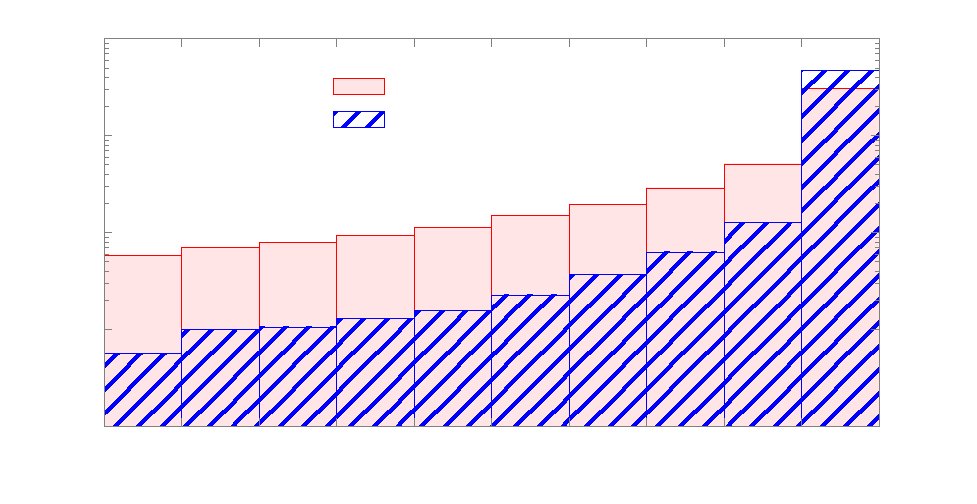
\includegraphics{figures/spectrum_angles_ee}}%
    \gplfronttext
  \end{picture}%
\endgroup
}

	\end{subfigure}

	\caption{\label{fig:spectrum_ee} \emph{Top} : Characteristic spectra for the total energy of observed  $e^+e^-$ pairs seen at \muboone\ produced in the $\ster \to \nu e^+e^-$ decay mode, for three representative masses. We see a preference for low energy events, with most events with energies below $0.4$ GeV. The modal peak of the distribution moves to higher energies as the mass of the sterile neutrino increases. On the left, the spectra have no analysis cuts or detector reconstruction effects applied, while on the right these are included, decreasing the discriminatory power of the lowest energy events.\\
		\emph{Bottom: }	 Same as above but for the angular spectrum (defined as the direction of the sum of their individual momenta) for a sterile neutrino mass of $m_\ster = 100$ MeV. The red histogram shows the true expected distribution, which we see is forward pointing. In blue we see the spectrum of events if we do not take into account the preferential
		decay rate for lower energy particles, instead using an energy independent
		decay rate. We see that this leads to a significantly more forward event 
		spectrum.	}
\end{figure}




\begin{figure}[t]
	%
	\center
		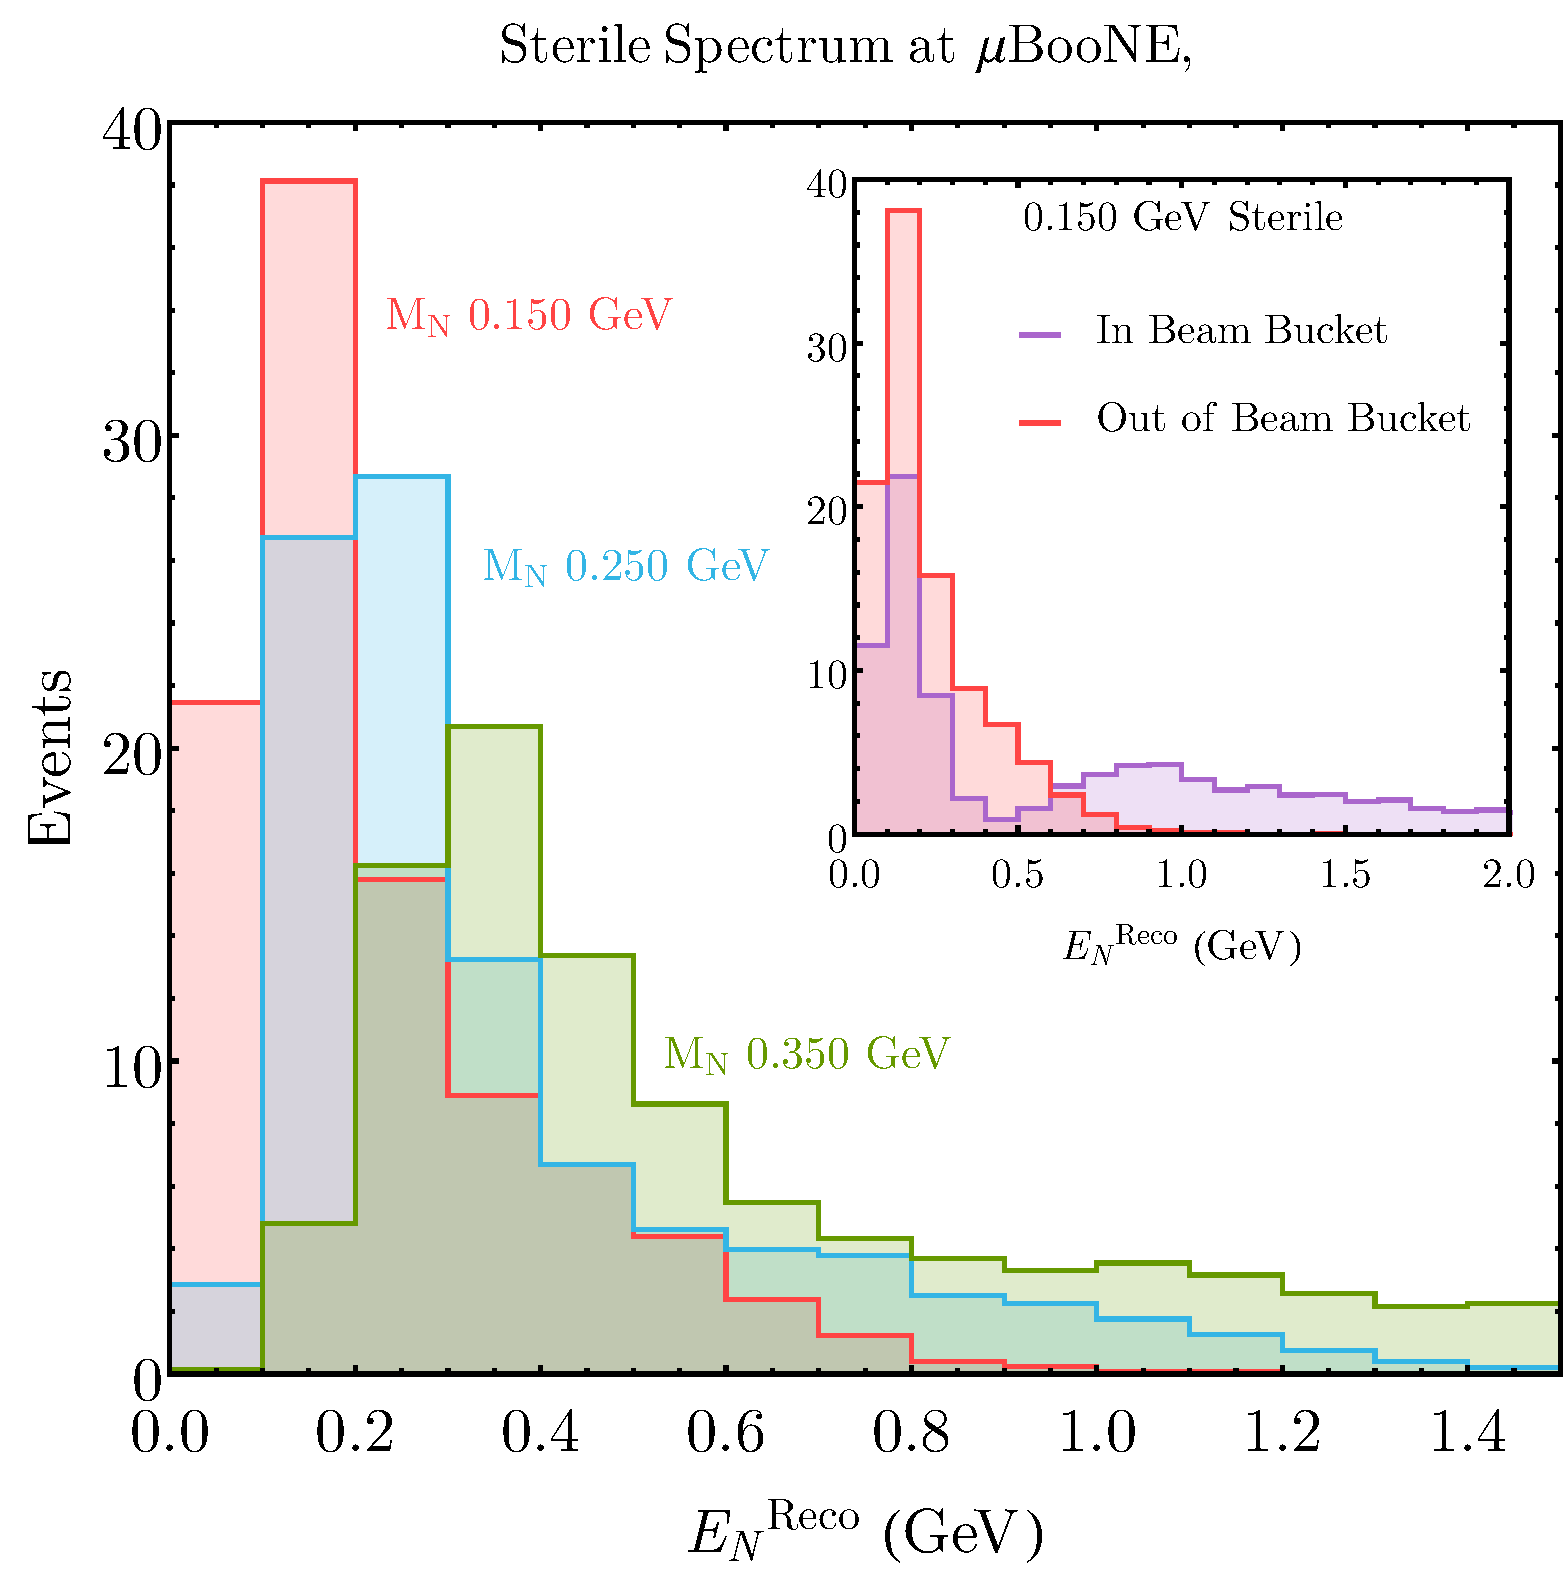
\includegraphics[width=0.5\textwidth]{figures/sterilecomparason.pdf}
	\caption{\label{fig:spectrum_epi} 
		The same characteristic spectra as \reffig{fig:spectrum_ee} for observed energy in the  $\ster\rightarrow e^\pm \pi^\mp$ decay mode for sterile neutrino masses of 150,
	250 and 350 MeV respectively. Now this energy is associated with the reconstructed sterile neutrino energy. One observes the exact same preference for low energy events and same qualitative behaviour as $m_\ster$ increases. This behaviour is common across all channels studied. Insert shows the stark differences in spectrum when on considers between events falling within the beam bucket window and without. }
	%
\end{figure}



%\begin{figure}[t]
%%
%\center
%%
%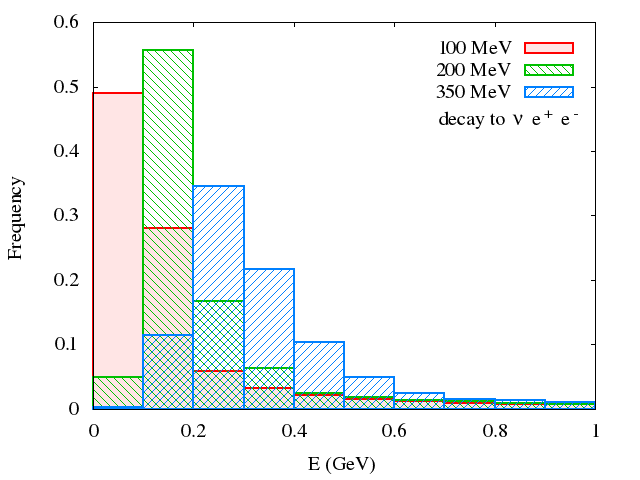
\includegraphics[width=0.47\textwidth]{figures/spectrum_ee_truth.png} 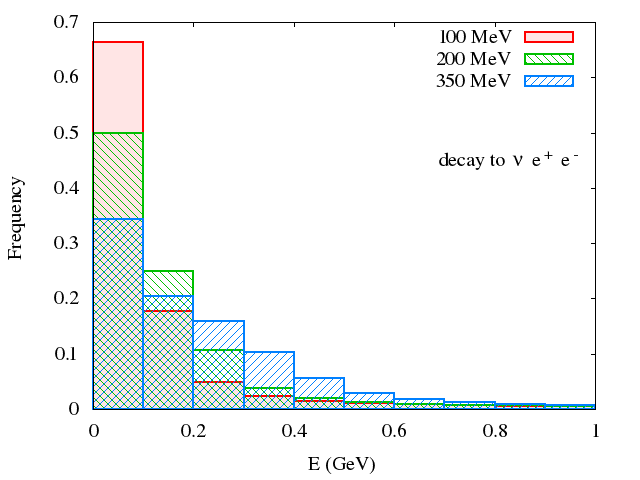
\includegraphics[width=0.47\textwidth]{figures/spectrum_ee_smeared.png}
%%
%\caption{\label{fig:spectrum_ee} Characteristic spectra for the total energy of observed  $e^+e^-$ pairs seen at \muboone\ produced in the $\ster \to \nu e^+e^-$ decay mode. The three distributions correspond to parent sterile masses given in the legend. We see a preference for low energy events, with most events with energies below $0.4$ GeV. On the left, we see the events without any detector resolution effects, and the distribution has a peak at low energies which is seen to move to higher energies as the mass of the sterile neutrino increases. On the right, a Gaussian smearing has been applied to the total energy. Here we see that the distributions are more uniform but the ratio of events above $0.2$ GeV could serve as a mass sensitive parameter.}
%%
%\end{figure}
% 
%\begin{figure}[t]
%%
%\center
%%
%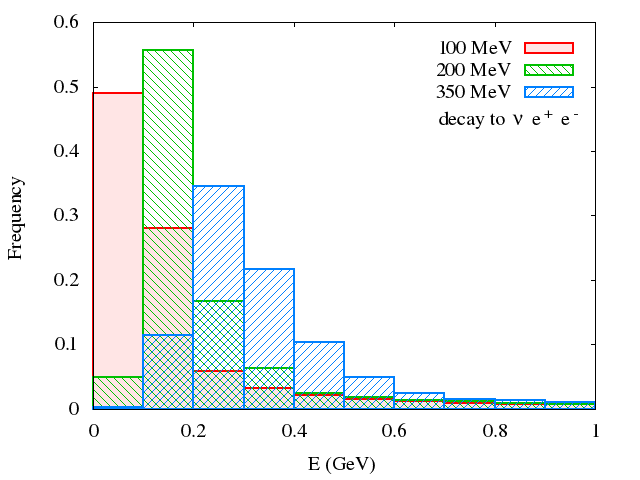
\includegraphics[width=0.47\textwidth]{figures/spectrum_ee_truth.png} 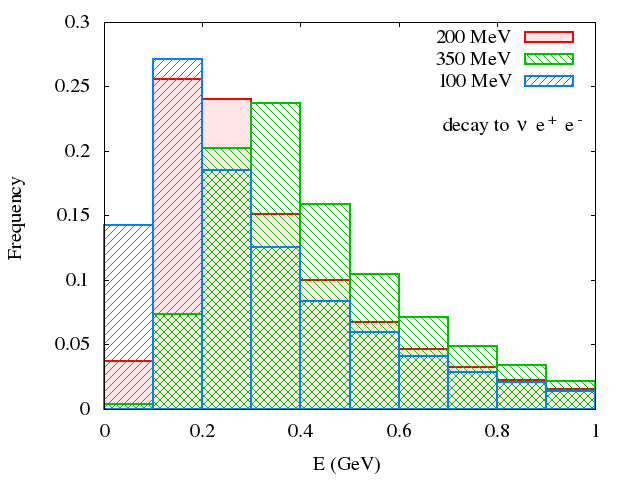
\includegraphics[width=0.47\textwidth]{figures/spectrum_ee_situ.png}
%%
%\caption{\label{fig:spectrum_ee} Characteristic spectra for the total energy of observed  $e^+e^-$ pairs seen at \muboone\ produced in the $\ster \to \nu e^+e^-$ decay mode by decay in flight (left) and by \emph{in situ} production and decay (right). The three distributions correspond to parent sterile masses given in the legend. We see a preference for low energy decay in flight events, with most events with energies below $0.4$ GeV, and the modal peak moving to higher energies as the parent mass increases. Although the same trend is seen for the \emph{in situ} production, low-energy suppression arising from the initial neutral current cross section produces a significantly broader distribution.}
%%
%\end{figure}
%
%

The differential distributions from heavy sterile neutrino decay tend to produce
distinctive low-energy distributions of events with an appreciably forward
direction. 
%
The tendency towards low energies is predominately due to the higher decay
rates of low-energy particles, which as can be seen in the previous section,
leads to factors of $1/E_\nu$ in the event rate formula \refeq{eq:prob_dec1}.
%
The forward trajectory in inherited from the kinematics of a boosted object
decaying in flight. However, this effect is mitigated by the preference for
lower energy decays, meaning that lower energy sterile neutrinnos are more likely to
decay, which are the least boosted objects.

We show an example of a distribution for electron-positron production in the
top left panel of \reffig{fig:spectrum_ee}. For the lowest masses that we consider, almost all events have
energies below $0.5$ GeV, in this case illustrated by the red histogram. The
distribution tends towards larger energies as the mass of the sterile neutrino
increases, but for sterile neutrino masses less than the kaon mass, never produces
significant numbers of events above $1$ GeV. As we can see in
\reffig{fig:spectrum_ee}, the number of events in the lowest energy bin is
strongly indicative of the mass of the parent particle, and therefore the
lowest energy events will play a strong role in model discrimination. However,
as can be seen in the top right panel of \reffig{fig:spectrum_ee}, in the
cut-based analysis which we outline in \refapp{app:bg} the lowest energy event
distribution is significantly reduced due to poor efficiencies at low-energy in
our cuts. In \reffig{fig:spectrum_epi} we show the same
distributions for electron-pion production, noting the same spectral features
of the electron-positron channel. Indeed this behaviour qualitatively exists in all channels studied. In the inset of \reffig{fig:spectrum_epi} we highlight the differences
that an accurate timing resolution can give, with the in-bucket and out of bucket
spectra showing very significant differences.  Through optimisation of this part of
the analysis, we can expect improvements in the sensitivity to these models;
however, this is beyond the scope of the present work.  



%%%%% This figure shows two spectra WITHOUT CUTS (left) and WITH CUTS (right)
%\begin{figure}[t]
%%
%\center
%%
%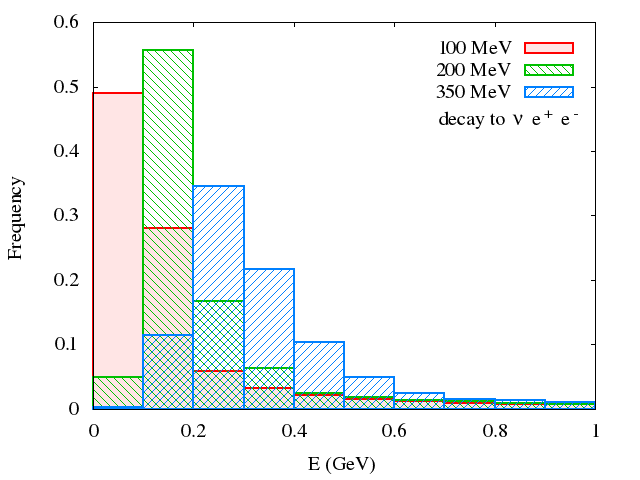
\includegraphics[width=0.47\textwidth]{figures/spectrum_ee_truth.png} 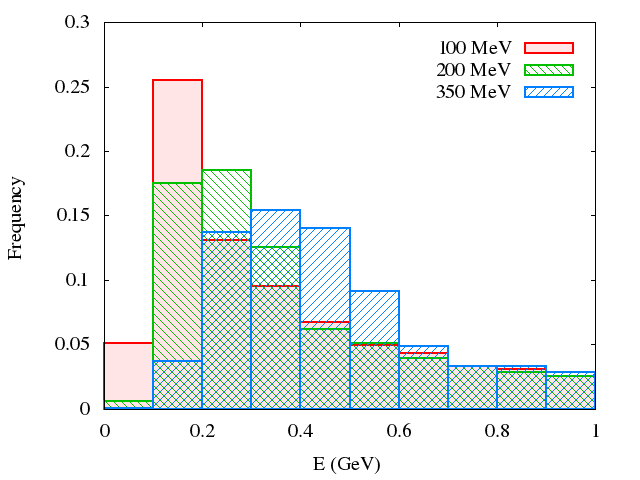
\includegraphics[width=0.47\textwidth]{figures/spectrum_ee_truth_cuts.png}
%%
%\caption{\label{fig:spectrum_ee} Characteristic spectra for the total energy of observed  $e^+e^-$ pairs seen at \muboone\ produced in the $\ster \to \nu e^+e^-$ decay mode. The three distributions correspond to parent sterile masses given in the legend. We see a preference for low energy events, with most events with energies below $0.4$ GeV. The modal peak of the distribution moves to higher energies as the mass of the sterile neutrino increases. On the left, the spectra have no analysis cuts or detector reconstruction effects applied, while on the right these are included, decreasing the discriminatory power of the lowest energy events.}
%%
%\end{figure}
%


%\begin{figure}[t]
%\begin{subfigure}[c]{0.5\textwidth}
%	\center
%	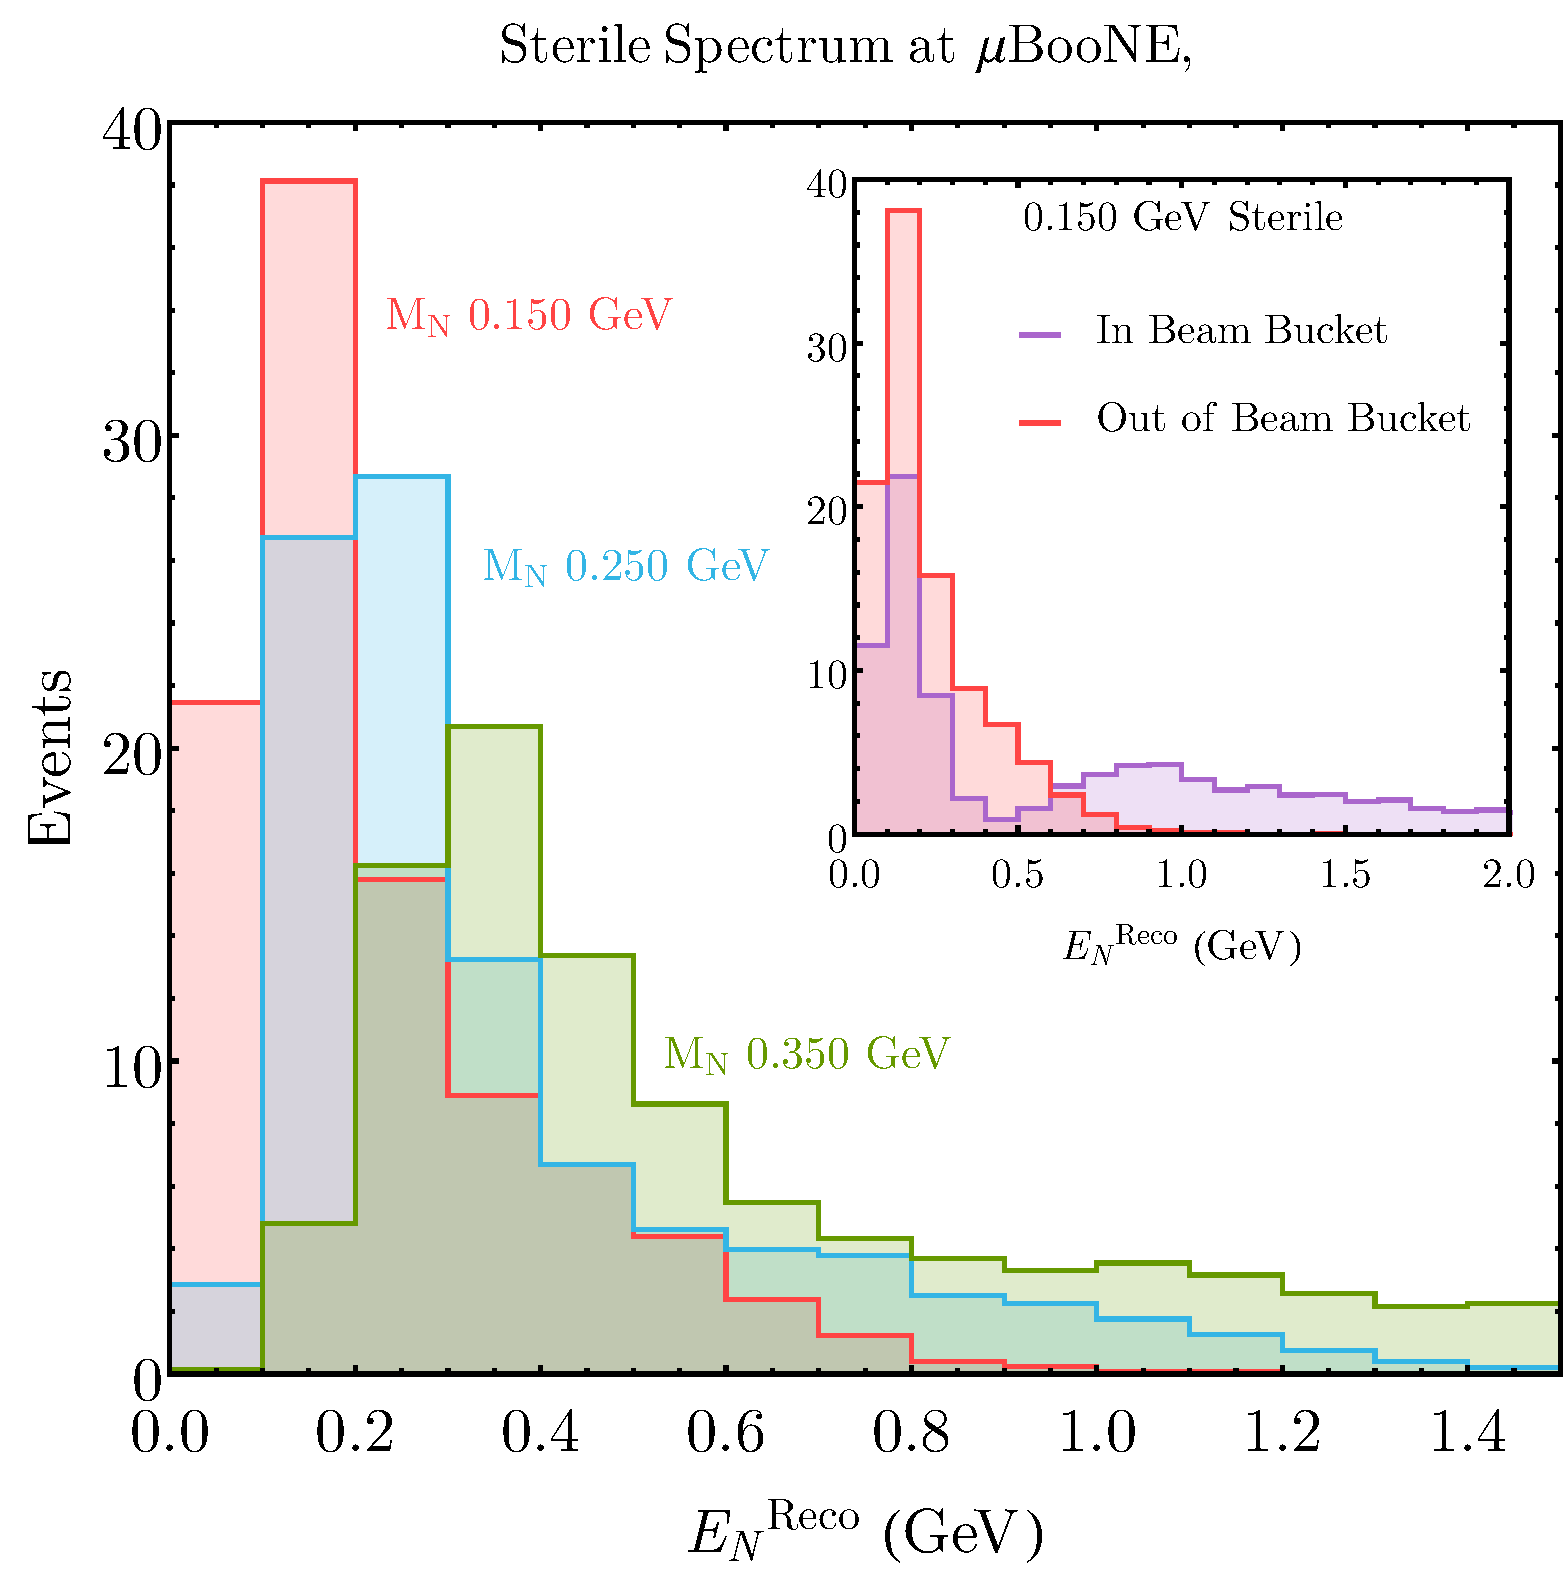
\includegraphics[width=\textwidth]{figures/sterilecomparason.pdf}
%\end{subfigure}
%\begin{subfigure}[c]{0.5\textwidth}
%	\center
	%\begin{subfigure}[t]{\textwidth}
	%	\large
	%	\resizebox{\columnwidth}{!}{% GNUPLOT: LaTeX picture with Postscript
\begingroup
  \fontfamily{ptm}%
  \selectfont
  \makeatletter
  \providecommand\color[2][]{%
    \GenericError{(gnuplot) \space\space\space\@spaces}{%
      Package color not loaded in conjunction with
      terminal option `colourtext'%
    }{See the gnuplot documentation for explanation.%
    }{Either use 'blacktext' in gnuplot or load the package
      color.sty in LaTeX.}%
    \renewcommand\color[2][]{}%
  }%
  \providecommand\includegraphics[2][]{%
    \GenericError{(gnuplot) \space\space\space\@spaces}{%
      Package graphicx or graphics not loaded%
    }{See the gnuplot documentation for explanation.%
    }{The gnuplot epslatex terminal needs graphicx.sty or graphics.sty.}%
    \renewcommand\includegraphics[2][]{}%
  }%
  \providecommand\rotatebox[2]{#2}%
  \@ifundefined{ifGPcolor}{%
    \newif\ifGPcolor
    \GPcolortrue
  }{}%
  \@ifundefined{ifGPblacktext}{%
    \newif\ifGPblacktext
    \GPblacktexttrue
  }{}%
  % define a \g@addto@macro without @ in the name:
  \let\gplgaddtomacro\g@addto@macro
  % define empty templates for all commands taking text:
  \gdef\gplbacktext{}%
  \gdef\gplfronttext{}%
  \makeatother
  \ifGPblacktext
    % no textcolor at all
    \def\colorrgb#1{}%
    \def\colorgray#1{}%
  \else
    % gray or color?
    \ifGPcolor
      \def\colorrgb#1{\color[rgb]{#1}}%
      \def\colorgray#1{\color[gray]{#1}}%
      \expandafter\def\csname LTw\endcsname{\color{white}}%
      \expandafter\def\csname LTb\endcsname{\color{black}}%
      \expandafter\def\csname LTa\endcsname{\color{black}}%
      \expandafter\def\csname LT0\endcsname{\color[rgb]{1,0,0}}%
      \expandafter\def\csname LT1\endcsname{\color[rgb]{0,1,0}}%
      \expandafter\def\csname LT2\endcsname{\color[rgb]{0,0,1}}%
      \expandafter\def\csname LT3\endcsname{\color[rgb]{1,0,1}}%
      \expandafter\def\csname LT4\endcsname{\color[rgb]{0,1,1}}%
      \expandafter\def\csname LT5\endcsname{\color[rgb]{1,1,0}}%
      \expandafter\def\csname LT6\endcsname{\color[rgb]{0,0,0}}%
      \expandafter\def\csname LT7\endcsname{\color[rgb]{1,0.3,0}}%
      \expandafter\def\csname LT8\endcsname{\color[rgb]{0.5,0.5,0.5}}%
    \else
      % gray
      \def\colorrgb#1{\color{black}}%
      \def\colorgray#1{\color[gray]{#1}}%
      \expandafter\def\csname LTw\endcsname{\color{white}}%
      \expandafter\def\csname LTb\endcsname{\color{black}}%
      \expandafter\def\csname LTa\endcsname{\color{black}}%
      \expandafter\def\csname LT0\endcsname{\color{black}}%
      \expandafter\def\csname LT1\endcsname{\color{black}}%
      \expandafter\def\csname LT2\endcsname{\color{black}}%
      \expandafter\def\csname LT3\endcsname{\color{black}}%
      \expandafter\def\csname LT4\endcsname{\color{black}}%
      \expandafter\def\csname LT5\endcsname{\color{black}}%
      \expandafter\def\csname LT6\endcsname{\color{black}}%
      \expandafter\def\csname LT7\endcsname{\color{black}}%
      \expandafter\def\csname LT8\endcsname{\color{black}}%
    \fi
  \fi
  \setlength{\unitlength}{0.0500bp}%
  \begin{picture}(11320.00,3400.00)%
    \gplgaddtomacro\gplbacktext{%
      \colorrgb{0.50,0.50,0.50}%
      \put(918,680){\makebox(0,0)[r]{\strut{} 0}}%
      \colorrgb{0.50,0.50,0.50}%
      \put(918,1045){\makebox(0,0)[r]{\strut{} 0.1}}%
      \colorrgb{0.50,0.50,0.50}%
      \put(918,1411){\makebox(0,0)[r]{\strut{} 0.2}}%
      \colorrgb{0.50,0.50,0.50}%
      \put(918,1776){\makebox(0,0)[r]{\strut{} 0.3}}%
      \colorrgb{0.50,0.50,0.50}%
      \put(918,2141){\makebox(0,0)[r]{\strut{} 0.4}}%
      \colorrgb{0.50,0.50,0.50}%
      \put(918,2507){\makebox(0,0)[r]{\strut{} 0.5}}%
      \colorrgb{0.50,0.50,0.50}%
      \put(918,2872){\makebox(0,0)[r]{\strut{} 0.6}}%
      \colorrgb{0.50,0.50,0.50}%
      \put(1020,494){\makebox(0,0){\strut{} 0}}%
      \colorrgb{0.50,0.50,0.50}%
      \put(1897,494){\makebox(0,0){\strut{} 0.2}}%
      \colorrgb{0.50,0.50,0.50}%
      \put(2774,494){\makebox(0,0){\strut{} 0.4}}%
      \colorrgb{0.50,0.50,0.50}%
      \put(3650,494){\makebox(0,0){\strut{} 0.6}}%
      \colorrgb{0.50,0.50,0.50}%
      \put(4527,494){\makebox(0,0){\strut{} 0.8}}%
      \colorrgb{0.50,0.50,0.50}%
      \put(5404,494){\makebox(0,0){\strut{} 1}}%
      \csname LTb\endcsname%
      \put(315,1776){\rotatebox{-270}{\makebox(0,0){\strut{}Frequency}}}%
      \csname LTb\endcsname%
      \put(5589,1776){\rotatebox{-270}{\makebox(0,0){\strut{}}}}%
      \csname LTb\endcsname%
      \put(3212,215){\makebox(0,0){\strut{}E (GeV)}}%
      \put(3212,2779){\makebox(0,0){\strut{}}}%
      \csname LTb\endcsname%
      \put(3212,2778){\makebox(0,0){\strut{}}}%
      \put(408,178){\makebox(0,0)[l]{\strut{}}}%
      \put(3650,1776){\makebox(0,0)[l]{\strut{}decay to $\nu e^+ e^-$}}%
    }%
    \gplgaddtomacro\gplfronttext{%
      \csname LTb\endcsname%
      \put(4616,2612){\makebox(0,0)[r]{\strut{}100 MeV}}%
      \csname LTb\endcsname%
      \put(4616,2426){\makebox(0,0)[r]{\strut{}200 MeV}}%
      \csname LTb\endcsname%
      \put(4616,2240){\makebox(0,0)[r]{\strut{}350 MeV}}%
    }%
    \gplgaddtomacro\gplbacktext{%
      \colorrgb{0.50,0.50,0.50}%
      \put(6578,680){\makebox(0,0)[r]{\strut{} 0}}%
      \colorrgb{0.50,0.50,0.50}%
      \put(6578,1045){\makebox(0,0)[r]{\strut{} 0.05}}%
      \colorrgb{0.50,0.50,0.50}%
      \put(6578,1411){\makebox(0,0)[r]{\strut{} 0.1}}%
      \colorrgb{0.50,0.50,0.50}%
      \put(6578,1776){\makebox(0,0)[r]{\strut{} 0.15}}%
      \colorrgb{0.50,0.50,0.50}%
      \put(6578,2141){\makebox(0,0)[r]{\strut{} 0.2}}%
      \colorrgb{0.50,0.50,0.50}%
      \put(6578,2507){\makebox(0,0)[r]{\strut{} 0.25}}%
      \colorrgb{0.50,0.50,0.50}%
      \put(6578,2872){\makebox(0,0)[r]{\strut{} 0.3}}%
      \colorrgb{0.50,0.50,0.50}%
      \put(6680,494){\makebox(0,0){\strut{} 0}}%
      \colorrgb{0.50,0.50,0.50}%
      \put(7557,494){\makebox(0,0){\strut{} 0.2}}%
      \colorrgb{0.50,0.50,0.50}%
      \put(8434,494){\makebox(0,0){\strut{} 0.4}}%
      \colorrgb{0.50,0.50,0.50}%
      \put(9310,494){\makebox(0,0){\strut{} 0.6}}%
      \colorrgb{0.50,0.50,0.50}%
      \put(10187,494){\makebox(0,0){\strut{} 0.8}}%
      \colorrgb{0.50,0.50,0.50}%
      \put(11064,494){\makebox(0,0){\strut{} 1}}%
      \csname LTb\endcsname%
      \put(5873,1776){\rotatebox{-270}{\makebox(0,0){\strut{}Frequency}}}%
      \csname LTb\endcsname%
      \put(11249,1776){\rotatebox{-270}{\makebox(0,0){\strut{}}}}%
      \csname LTb\endcsname%
      \put(8872,215){\makebox(0,0){\strut{}E (GeV)}}%
      \put(8872,2779){\makebox(0,0){\strut{}}}%
      \csname LTb\endcsname%
      \put(8872,2778){\makebox(0,0){\strut{}}}%
      \put(5966,178){\makebox(0,0)[l]{\strut{}}}%
      \put(9310,1776){\makebox(0,0)[l]{\strut{}decay to $\nu e^+ e^-$}}%
    }%
    \gplgaddtomacro\gplfronttext{%
      \csname LTb\endcsname%
      \put(10276,2612){\makebox(0,0)[r]{\strut{}100 MeV}}%
      \csname LTb\endcsname%
      \put(10276,2426){\makebox(0,0)[r]{\strut{}200 MeV}}%
      \csname LTb\endcsname%
      \put(10276,2240){\makebox(0,0)[r]{\strut{}350 MeV}}%
    }%
    \gplbacktext
    \put(0,0){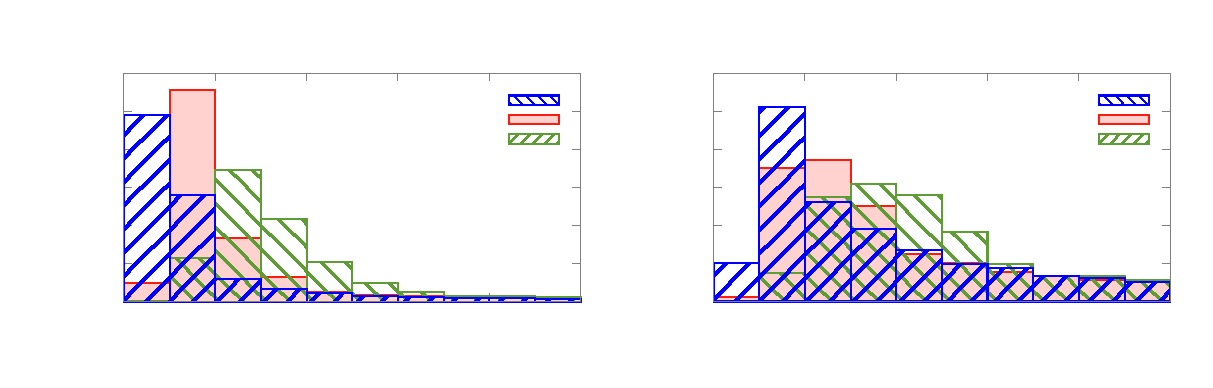
\includegraphics{figures/spectrum}}%
    \gplfronttext
  \end{picture}%
\endgroup
}
	%\end{subfigure}
%	\begin{subfigure}[b]{\textwidth}
%		\Large
%		\resizebox{\columnwidth}{!}{% GNUPLOT: LaTeX picture with Postscript
\begingroup
  \fontfamily{ptm}%
  \selectfont
  \makeatletter
  \providecommand\color[2][]{%
    \GenericError{(gnuplot) \space\space\space\@spaces}{%
      Package color not loaded in conjunction with
      terminal option `colourtext'%
    }{See the gnuplot documentation for explanation.%
    }{Either use 'blacktext' in gnuplot or load the package
      color.sty in LaTeX.}%
    \renewcommand\color[2][]{}%
  }%
  \providecommand\includegraphics[2][]{%
    \GenericError{(gnuplot) \space\space\space\@spaces}{%
      Package graphicx or graphics not loaded%
    }{See the gnuplot documentation for explanation.%
    }{The gnuplot epslatex terminal needs graphicx.sty or graphics.sty.}%
    \renewcommand\includegraphics[2][]{}%
  }%
  \providecommand\rotatebox[2]{#2}%
  \@ifundefined{ifGPcolor}{%
    \newif\ifGPcolor
    \GPcolortrue
  }{}%
  \@ifundefined{ifGPblacktext}{%
    \newif\ifGPblacktext
    \GPblacktexttrue
  }{}%
  % define a \g@addto@macro without @ in the name:
  \let\gplgaddtomacro\g@addto@macro
  % define empty templates for all commands taking text:
  \gdef\gplbacktext{}%
  \gdef\gplfronttext{}%
  \makeatother
  \ifGPblacktext
    % no textcolor at all
    \def\colorrgb#1{}%
    \def\colorgray#1{}%
  \else
    % gray or color?
    \ifGPcolor
      \def\colorrgb#1{\color[rgb]{#1}}%
      \def\colorgray#1{\color[gray]{#1}}%
      \expandafter\def\csname LTw\endcsname{\color{white}}%
      \expandafter\def\csname LTb\endcsname{\color{black}}%
      \expandafter\def\csname LTa\endcsname{\color{black}}%
      \expandafter\def\csname LT0\endcsname{\color[rgb]{1,0,0}}%
      \expandafter\def\csname LT1\endcsname{\color[rgb]{0,1,0}}%
      \expandafter\def\csname LT2\endcsname{\color[rgb]{0,0,1}}%
      \expandafter\def\csname LT3\endcsname{\color[rgb]{1,0,1}}%
      \expandafter\def\csname LT4\endcsname{\color[rgb]{0,1,1}}%
      \expandafter\def\csname LT5\endcsname{\color[rgb]{1,1,0}}%
      \expandafter\def\csname LT6\endcsname{\color[rgb]{0,0,0}}%
      \expandafter\def\csname LT7\endcsname{\color[rgb]{1,0.3,0}}%
      \expandafter\def\csname LT8\endcsname{\color[rgb]{0.5,0.5,0.5}}%
    \else
      % gray
      \def\colorrgb#1{\color{black}}%
      \def\colorgray#1{\color[gray]{#1}}%
      \expandafter\def\csname LTw\endcsname{\color{white}}%
      \expandafter\def\csname LTb\endcsname{\color{black}}%
      \expandafter\def\csname LTa\endcsname{\color{black}}%
      \expandafter\def\csname LT0\endcsname{\color{black}}%
      \expandafter\def\csname LT1\endcsname{\color{black}}%
      \expandafter\def\csname LT2\endcsname{\color{black}}%
      \expandafter\def\csname LT3\endcsname{\color{black}}%
      \expandafter\def\csname LT4\endcsname{\color{black}}%
      \expandafter\def\csname LT5\endcsname{\color{black}}%
      \expandafter\def\csname LT6\endcsname{\color{black}}%
      \expandafter\def\csname LT7\endcsname{\color{black}}%
      \expandafter\def\csname LT8\endcsname{\color{black}}%
    \fi
  \fi
  \setlength{\unitlength}{0.0500bp}%
  \begin{picture}(9060.00,4520.00)%
    \gplgaddtomacro\gplbacktext{%
      \csname LTb\endcsname%
      \put(533,2455){\rotatebox{-270}{\makebox(0,0){\strut{}Frequency}}}%
      \csname LTb\endcsname%
      \put(8456,2455){\rotatebox{-270}{\makebox(0,0){\strut{}}}}%
      \csname LTb\endcsname%
      \put(4550,130){\makebox(0,0){\strut{}$\cos\theta$}}%
      \put(4550,4222){\makebox(0,0){\strut{}}}%
      \csname LTb\endcsname%
      \put(4550,4221){\makebox(0,0){\strut{}}}%
      \put(626,93){\makebox(0,0)[l]{\strut{}}}%
      \put(1425,3105){\makebox(0,0)[l]{\strut{}$m_N = 100$ MeV}}%
    }%
    \gplgaddtomacro\gplfronttext{%
      \csname LTb\endcsname%
      \put(2934,3856){\makebox(0,0)[r]{\strut{}true decay rate}}%
      \csname LTb\endcsname%
      \put(2934,3540){\makebox(0,0)[r]{\strut{}flat decay rate}}%
      \colorrgb{0.50,0.50,0.50}%
      \put(728,1525){\makebox(0,0)[r]{\strut{}}}%
      \colorrgb{0.50,0.50,0.50}%
      \put(728,2455){\makebox(0,0)[r]{\strut{}}}%
      \colorrgb{0.50,0.50,0.50}%
      \put(728,3385){\makebox(0,0)[r]{\strut{}}}%
      \colorrgb{0.50,0.50,0.50}%
      \put(728,4315){\makebox(0,0)[r]{\strut{}}}%
      \colorrgb{0.50,0.50,0.50}%
      \put(830,409){\makebox(0,0){\strut{} 0}}%
      \colorrgb{0.50,0.50,0.50}%
      \put(1574,409){\makebox(0,0){\strut{} 0.1}}%
      \colorrgb{0.50,0.50,0.50}%
      \put(2318,409){\makebox(0,0){\strut{} 0.2}}%
      \colorrgb{0.50,0.50,0.50}%
      \put(3062,409){\makebox(0,0){\strut{} 0.3}}%
      \colorrgb{0.50,0.50,0.50}%
      \put(3806,409){\makebox(0,0){\strut{} 0.4}}%
      \colorrgb{0.50,0.50,0.50}%
      \put(4551,409){\makebox(0,0){\strut{} 0.5}}%
      \colorrgb{0.50,0.50,0.50}%
      \put(5295,409){\makebox(0,0){\strut{} 0.6}}%
      \colorrgb{0.50,0.50,0.50}%
      \put(6039,409){\makebox(0,0){\strut{} 0.7}}%
      \colorrgb{0.50,0.50,0.50}%
      \put(6783,409){\makebox(0,0){\strut{} 0.8}}%
      \colorrgb{0.50,0.50,0.50}%
      \put(7527,409){\makebox(0,0){\strut{} 0.9}}%
      \colorrgb{0.50,0.50,0.50}%
      \put(8271,409){\makebox(0,0){\strut{} 1}}%
    }%
    \gplbacktext
    \put(0,0){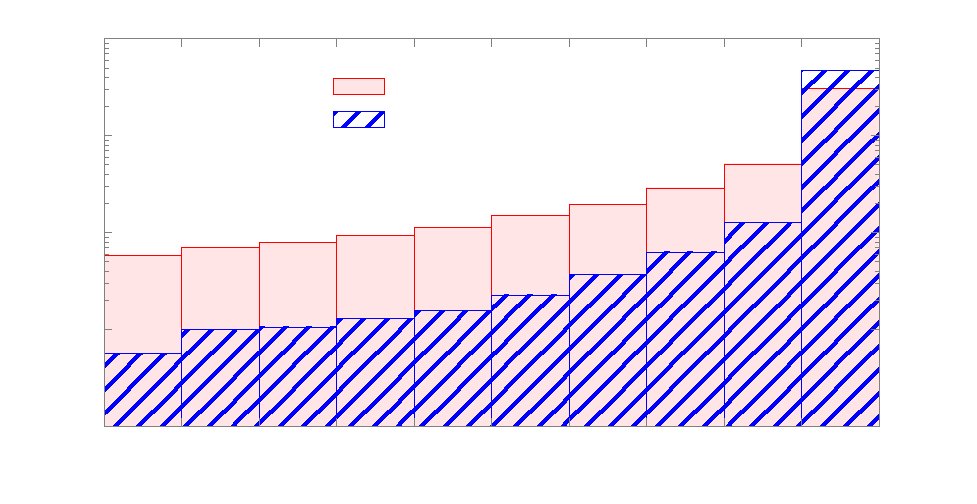
\includegraphics{figures/spectrum_angles_ee}}%
    \gplfronttext
  \end{picture}%
\endgroup
}
%	\end{subfigure}
%\end{subfigure}
%
%
%\caption{\label{fig:spectrum_ee} \emph{Left: } Characteristic spectra for the total energy of observed  $e^+e^-$ pairs seen at \muboone\ produced in the $\ster \to \nu e^+e^-$ decay mode. The three distributions correspond to parent sterile masses given in the legend. We see a preference for low energy events, with most events with energies below $0.4$ GeV. The modal peak of the distribution moves to higher energies as the mass of the sterile neutrino increases. Insert shows the stark differences in spectrum when on considers between events falling within the beam bucket window and without. 
%\emph{Right Top: }  The same characteristic spectra for observed energy in the  $\ster\rightarrow e^\pm \pi^\mp$ decay mode for sterile masses of 150,
%250 and 350 MeV respectively. We include the effect of analysis cuts and detector reconstruction effects on the spectra, decreasing the overall discriminatory power of the lowest energy events.
%\emph{Right: } The angular spectrum of $e^+e^-$ events (defined as the direction of the sum of their individual momenta) in
%\muboone\ for a sterile neutrino mass of $m_N = 100$ MeV. The red histogram
%shows the true expected distribution, which we see is forward pointing. In blue
%we see the spectrum of events if we do not take into account the preferential
%decay rate for lower energy particles, instead using an energy independent
%decay rate. We see that this leads to a significantly more forward event 
%spectrum. 
%\end{figure}



%
%Although both models produce visible particles through sterile neutrino decay
%in flight, the additional neutral current cross-section required by the
%Gninenko-type sterile suppresses the lowest energy events. As can be seen in
%\reffig{fig:XXX}, we see a marked difference between these signals at SBND. If
%we factor in the cut-based analysis that was performed in the preceeding
%section, we see that the model in this paper does lose a significant number of
%events from the lowest bins. To separate these events cleanly, the analysis
%should be optimised to keep as many of these lowest energy events as possible. 
%
%

\section{\label{sec:sensitivities}Results}

In this section we present the results of our simulation. We have have
performed two analyses. In the first, we compute exclusion contours which could
be expected to be set by SBN if no signal is seen. We compute these for all
decay modes presented in \reffig{fig:branchingratios}. Our second analysis
considers the phenomenological potential of energy and timing spectral information at the SBN
experiment if an potential signal is observed. 

It must be pointed out that although \muboone\ contributes the least to the raw
number of sterile neutrino events expected, the MicroBooNE experiment is
significantly more advanced than its two SBN counterparts. At the time of
writing, \muboone\ has already collected close to $50$\% of its planned POT
(around $3.5\times 10^{20}$ POT) and has already presented its first results on
$\nu_\mu$ CC inclusive and $\nu_\mu$ CC$\pi^0$ \cite{mubooneneutrino}. As such
\muboone\ is in a unique position in that it has the potential to observe any
excess in advance of SBND or ICARUS and thus to inform a possible search using
the full SBN programme.
%
%While any observation of $\approx$100 events in \muboone consistent with a 300
%MeV sterile decaying $\nu_\ster \rightarrow \nu_\mu \pi^0$ (corresponding to
%$|U_{\mu 4}|^2 \approx 10^{-7.2}$) would mean that SBND will expect to see
%$\approx 2000$ events for the same parameter space, \muboone\ would see such a
%signal several years before SBND.
%
Non-observation of any excess at MicroBooNE would not negatively effect the
program for a subsequent search at SBND or ICARUS \newtext{PB}{as a large
fraction of the testable parameter space is not accessible to MicroBooNE.}

\subsection{SBN upper limits on sterile neutrino mixing}
%
\reffig{fig:band_sbn} presents the results of this analysis for the combined
$6.6\times 10^{20}$ POT exposure at SBND and ICARUS, and $13.2\times10^{20}$
POT at \muboone. The figure shows the predicted upper limits on sterile
neutrino mixing for the leptonic decay channels $\ster \rightarrow \nu_\alpha
e^+e^-$, $\ster \rightarrow \nu_\alpha \mu^+ \mu^- $ and $\ster \rightarrow
\nu_\alpha \mu^+ \mu^- $ as well as the semi-leptonic and photonic channels
$\ster \rightarrow \alpha^\mp \pi^\pm$,  $\ster \rightarrow \nu_\alpha \pi^0$
and $\ster \rightarrow \nu_\alpha \gamma$. \newtext{PB}{The plot on the right
assumes mixing with muon neutrinos and that on the left with electron
neutrinos.}
%
%for $|U_{\mu 4}|$ driven mixing in the right column, and $|U_{e4}|$ driven
%mixing  in the left column.  
%
The lower solid coloured lines are the background-less 90\% C.L upper limit
contours defined as 2.44 events following the procedure of
\refref{Feldman:1997qc} designed for background-less searches for rare events.
This represents the best expected sensitivity at the SBN program, assuming
perfect signal efficiency.  We also present the results of the cut based
background analysis discussed in \refsec{sec:backgroundestimate} (upper solid
coloured lines).  
%
Depending on the optimisation of the analysis, including the possibility of
using improved timing information, we expect the ultimate sensitivity to be
within the solid-shaded region, lying between the proven cut-based sensitivity
and the backgroundless one. \marcom{PB}{Added S.'s comments up to here.}

We see that the increased event rates at the SBN program compared to PS-191
allows an improvement of the bounds on $|U_{e4}|^2$ and $|U_{\mu 4}|^2$ in all
channels studied over wide regions of parameter space. The strongest bounds
come from the semi-leptonic $\ster \rightarrow l^\pm \pi^\mp$ searches, where
mixing matrix elements greater than $|U_{e4}|^2 \leq 10^{-9}$ can be excluded
at the 90\% C.L for $m_\ster \approx 0.350$ GeV. The bounds have the potential
to improve upon the $\pi^-$ peak search bounds on for $m_\ster \leq 0.033$ MeV
and $\leq 0.138$ for muon and electron mixing respectively, if the backgrounds
can be further suppressed, possibly through the use of timing information.

Additionally, we show that the previously poorly bounded photonic-like
channels $\ster \rightarrow \nu_\alpha \pi^0$ and $\ster \rightarrow \nu_\alpha
\gamma$ can be probed across the entire parameter space studied providing new
constraints on exotic sterile neutrino signatures. The potential beam-related
backgrounds are larger in these photonic channels, the effect of which is a
much wider spread in achievable limits. These photonic channels allow SBN to
probe the electromagnetic nature of the sterile neutrino, placing bounds on any
models containing enhanced anomalous magnetic moments. 
%
For sterile neutrinos whose mass lies  $m_\pi^0 \leq m_\ster \leq m_\pi^\pm +m_\mu$ the
$\ster \rightarrow \nu_\mu \pi^0$ channel can extend the limits beyond that of
the traditional $e^+e^-$ searches to probe new parameter space, even in the
purely minimal model. In the case of electron mixing the $\pi^0$ bounds are
less powerful than that of the semi-leptonic $\ster \rightarrow e^\pm \pi^\mp$
when one solely considers the minimal model.

Although we have plotted the limits on mixing angles in \reffig{fig:band_sbn}
in terms of the parameters of the minimal model, they are model independent in
the sense that an a non-minimally enhanced decay rate in that channel would
just alter the interpretation of the $y$-axis. To reinterpret any bounds on
\reffig{fig:band_sbn} in the context of a non-minimal extension in which the
channel of interest is enhanced by $(1+\alpha)$ then the quantity bounded on
each vertical axis is given by  $|U_{\alpha 4}|^2/\sqrt{1+\alpha}$ $(\approx
|U_{\alpha 4}|^2/\sqrt{\alpha} $ for large $\alpha$) as discussed in
\refsec{sec:bounds}.  


\begin{figure}[t]
\center
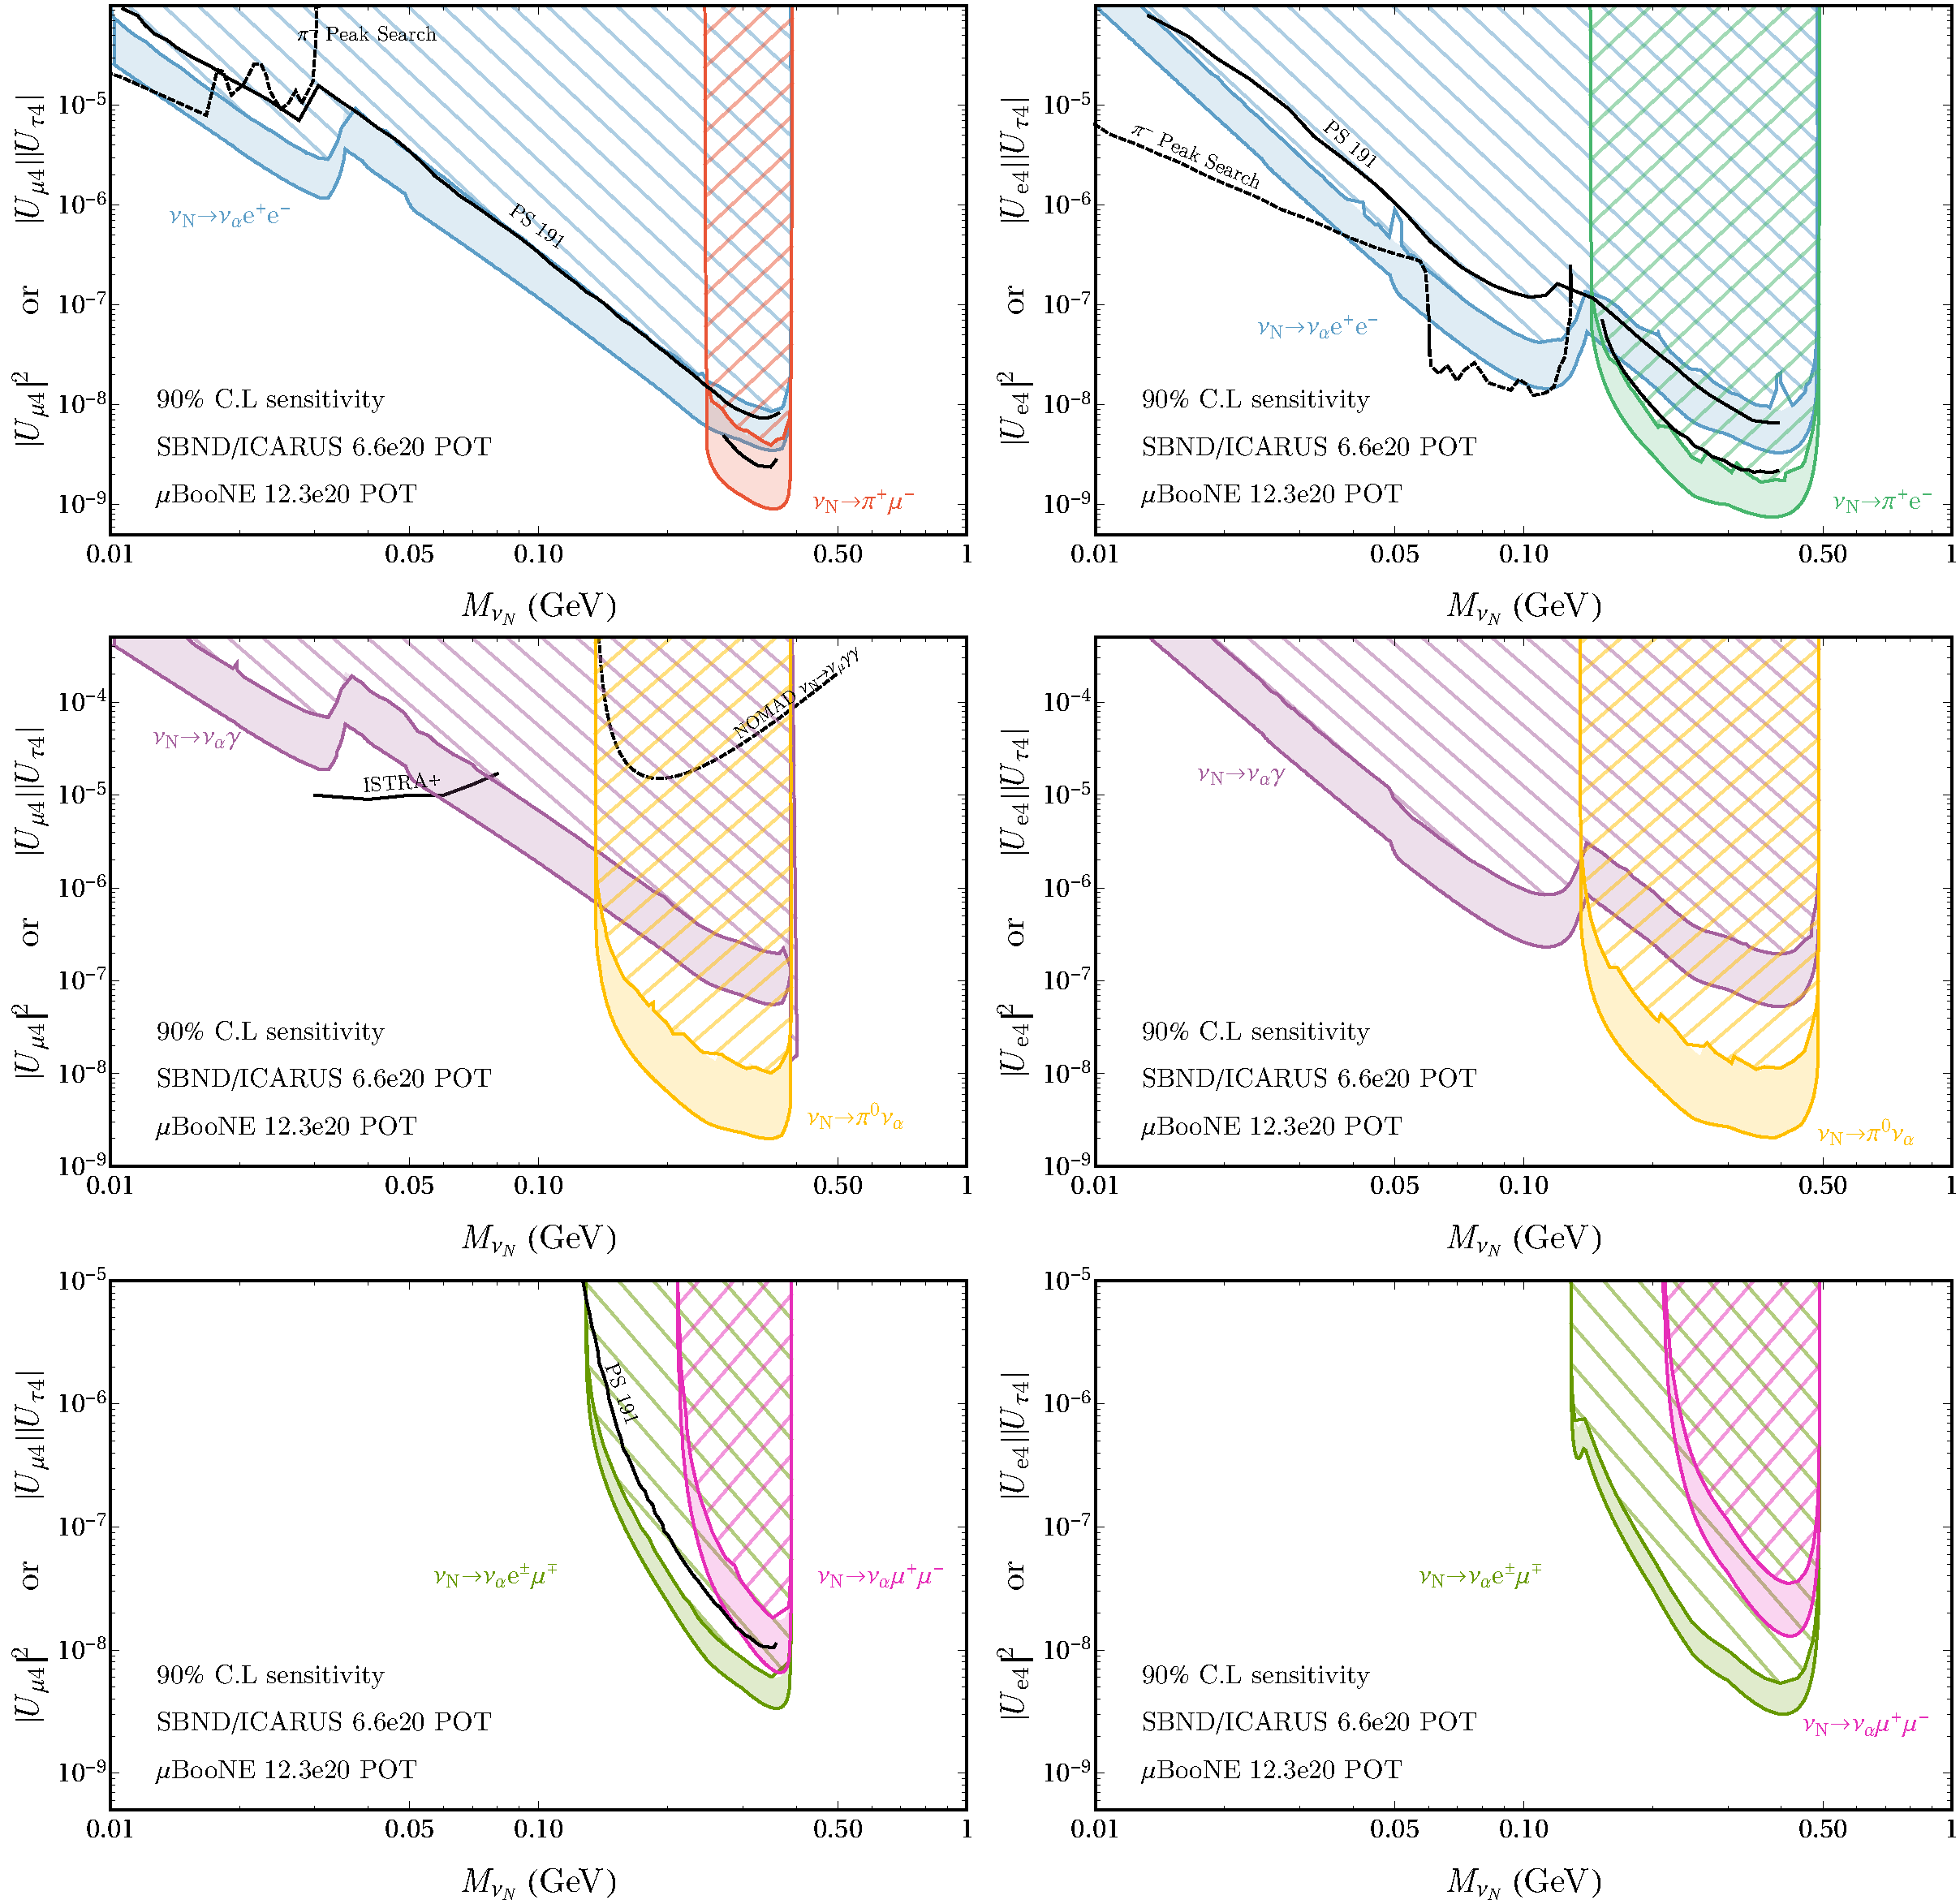
\includegraphics[width=1.0\textwidth]{figures/band_sbn_new.pdf}

\caption{\label{fig:band_sbn}The predicted  90\% C.L  upper limit contours for
the combined SBN detectors. Shown also in black solid lines is the prior best
bounds from PS-191, scaled to show bounds on the minimal extension as discussed
here, as well as bounds from lepton peak searches in pion and kaon decay
\cite{PhysRevD.46.R885,PhysRevLett.68.3000} (dashed black lines) . Note that the
peak searches are only valid when bounding pure mixing combinations, e.g
$|U_{\mu 4}|^2$ and not $|U_{\mu 4}||U_{\tau 4}|$ . In all panels, the mixing
matrix elements not shown on the $y$-axis are zero. Above we have the
previously bounded channels, $e^+e^-$ and $l^- \pi^+$ for nonzero $U_{\mu 4}$
and $U_{e4}$ respectively. In the middle row we have the same for the $\gamma$
and $\pi^0$ channels, and the bottom row we show the bounds on the leptonic
channels, $\mu^\pm e^\mp$ and $\mu^+ \mu^-$  . The photonic channels have
little or no direct bounds, with ISTRA+ bounding the radiative
decay \cite{Duk:2011yv} and reinterpreted $\ster \rightarrow \nu \gamma \gamma$
bounds at NOMAD on $\ster \rightarrow \nu \pi^0$ \cite{Gninenko:1998nn}. See
text for more details. }

\end{figure}

\subsection{\label{sec:timing_physics}Constraining an observed signal}

In addition to being able to reduce beam-related backgrounds, a precise
knowledge of the timing of any observed events can also be used to discriminate
between potential models and aid in parameter estimation. In the event that a
potential signal is indeed observed, the logical initial step would be to
confirm that the excess is indeed from a heavy particle propagating the
baseline before decaying. Accurate timing is a crucial tool in this, as an
energy analysis alone is not capable of providing a strong enough case that the
events arise from a decay-in-flight even if the energy spectrum is consistent.
Using energy alone we could not discount mis-understood beam-related
backgrounds, unknown nuclear effects or alternative models that mimic the
energy spectrum. As we expect all beam-related backgrounds to be in line with
the booster proton buckets, observation of events with timing inconsistent with
a Gaussian around the BNB beam bucket is a smoking gun signal of a sub-luminal
propagating parent. 

We estimate the required time resolution that demonstrates such a disagreement
with beam-related models via a Monte-Carlo analysis, simulating
such a decaying sterile neutrino and analysing the generated data under both the
decay-in-flight hypothesis as well as a beam-bucket-model hypothesis.  This
beam-bucket-model is shape only, always generating the correct rate and
encompasses all models (and backgrounds) that would generate a signal in time
with the neutrino beam and associated backgrounds. It assumes that all events
originate in the 6ns window surrounding the BNB beam spill, all smeared
according to an assumed time resolution. We define our test statistic  as
\cite{Agashe:2014kda} \[ t_m = -2 \ln \left(\mathcal{L}\right) =  2
\sum_{i=1}^N \left[ \mu_i(m)-n_i +n_i \ln(\frac{n_i}{\mu_i(m)})  \right], \]
where $\mu_i(m)$ is the expected number of events in bin $i$ if the sterile neutrino is
of mass $m$. Using this statistic we have run a binned
Maximum Likelihood analysis of the reconstructed time of arrival $\Delta T$,
assuming events are Poisson distributed.  As many bins contain low
if any events, as well as the cyclic nature of $\Delta T$ we have elected to
perform a Monte Carlo estimation of the distribution of $t_m$ simulating the
entire experiment many thousand times in order to account for any
non-gaussianity in the likelihood distributions. 

As the timing is solely a function of initial sterile neutrino energy and
mass, these results hold for all channels studied. In particular in \reffig{fig:hockey} we present results for the semi-leptonic channel $\ster \rightarrow e^\pm \pi^\mp$.  On the left we assume ICARUS observes an excess of 100 events due to a 300 MeV sterile neutrino. To guarantee that ICARUS obtains at least a $3\sigma$
significant rejection of the beam-window hypothesis 95\% of the time it would require a timing resolution of $\leq$ 3.5 ns. The greater the observed
excess allows for a proportionally less stringent timing resolution, as can be seen in the right-hand plot of \reffig{fig:hockey}, which in turn would allow for less parameter space to be probed at the same level.

\begin{figure}[t]
\center
\begin{subfigure}[t]{0.5\textwidth}
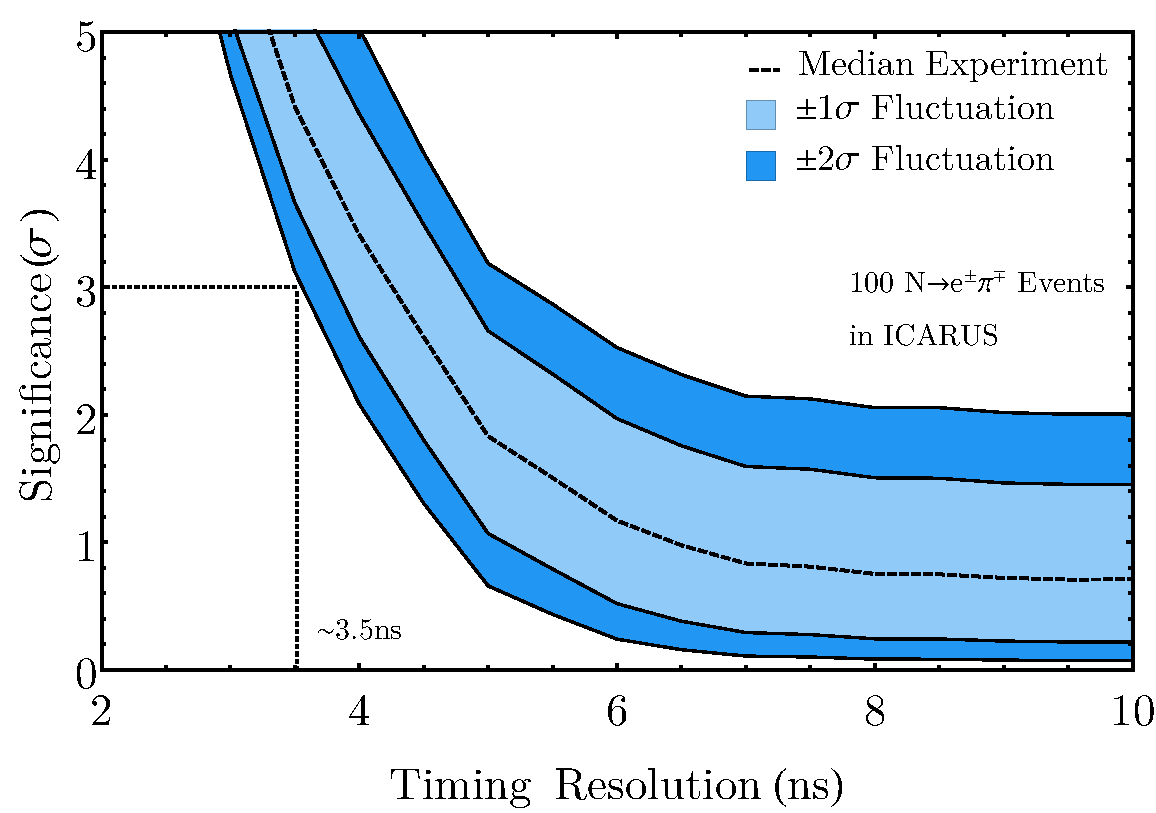
\includegraphics[width=\textwidth]{figures/hockey_plot.pdf}
\end{subfigure}%
~
\begin{subfigure}[t]{0.5\textwidth}
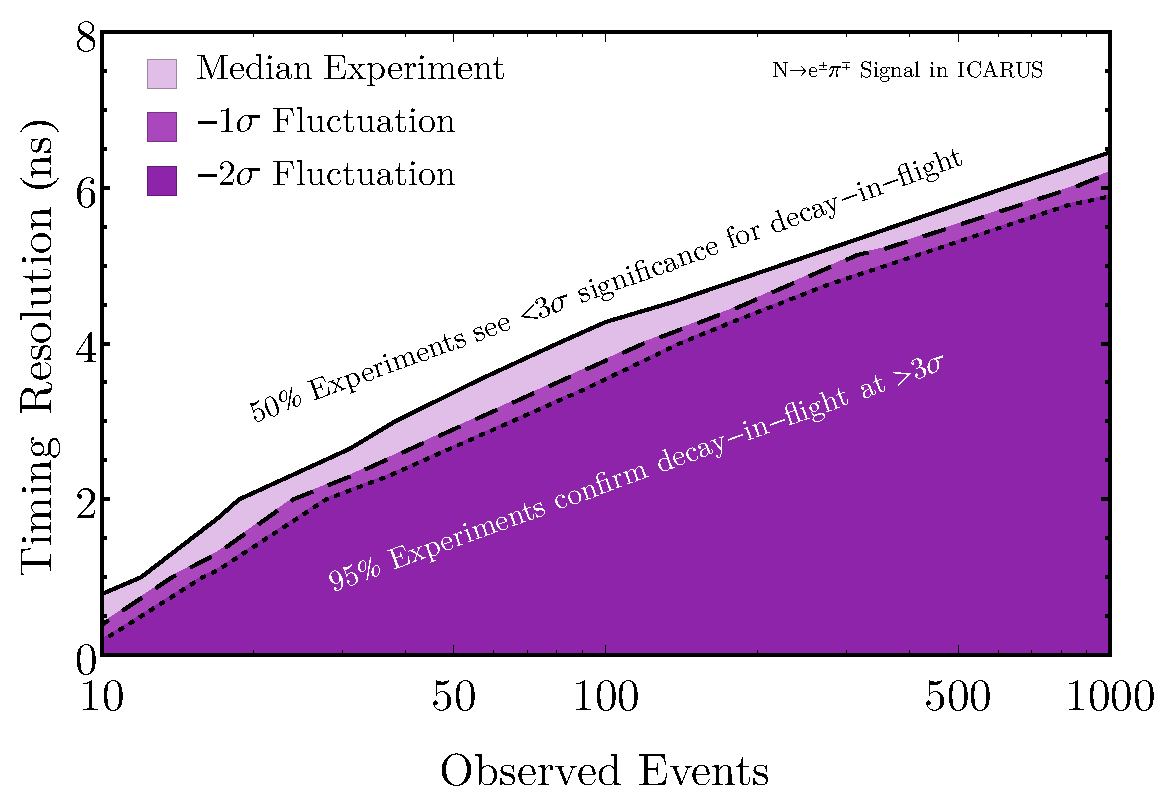
\includegraphics[width=\textwidth]{figures/icarus_contour.pdf}
\end{subfigure}
\caption{\label{fig:hockey}
\emph{Left:} Expected significance by which ICARUS can exclude an excess to be associated with the beam-bucket, in favour of a temporally delayed decay-in-flight model as a function of timing resolution. This assumes a hypothetical signal of 100 observed $e^\pm \pi^\mp$ events potentially consistent with $\ster \rightarrow e^\pm \pi^\mp$. If we want to ensure a $3\sigma$ significance ~95\% of the time one requires $~3.5$ ns timing resolution. \emph{Right:} Regions in the ``Signal Strength''-``Timing Resolution'' plane that ICARUS could exclude such a beam-window model in favour of a decay-in-flight for the median experiment (Solid) as well as for 1$\sigma$ (Dashed) and 2$\sigma$ (Dotted) downward fluctuations respectively, for the same $\ster \rightarrow e^\pm \pi^\mp$ signal.}

\end{figure}

Although such an observation and confirmation of events falling outside the beam-bucket
would be a strong hint of new physics, observation in one detector alone (such as
SBND with the largest statistics, or MicroBooNE which potentially could see a signal first)
would not be sufficient to claim discovery of such a decay-in-flight model due to
heavy particle propagation. If an unaccounted for background had a fixed time
delay with respect to the neutrino-beam $\Delta_t$, such as the relaxation time
of an excited atom, it could produce events in the inter-bucket window
if $\Delta_t \approx \mathcal{O}$(ns). Luckily the SBN programme has multiple
detectors at multiple baselines. A constant fixed time delay would produce
identical temporal signals in both SBND and ICARUS, where as if the observed
excess is indeed from a propagating particle then it would have to travel
approximately 6 times further to ICARUS leading to higher energy events populating further
and further from the beam-window. This effect is clearly shown in
\reffig{fig:icarus_the_great} where the ratio of events at SBND and ICARUS are
plotted showing the distortion due to increased travel distance. A constant
time delay would produce a ratio of 1 and curves that lie on the grey circle.
Measuring this distortion would be definitive proof of the heavy particle
having propagated the distance from target to detector and not merely being
produced \emph{in situ}.

This comparison of timing between the detectors also allows SBN to distinguish
a decay-in-flight model from other BSM scenarios involving heavy steriles. As an
example, the scenario described in \refref{Gninenko:2009ks,Gninenko:2010pr}
considers a sterile neutrino produced inside the detector through neutral
current scattering of an active neutrino. The heavy particle promptly
decays, with a decay length of the order $\mathcal{O}$(1)~m, producing the
visible signal. Although the sterile neutrinos are produced inside the detector with no
timing delay, the finite lifetime of these particles could lead to events
falling in the inter-bucket window. However, as it is active neutrinos which propagate in this scenario, the delay could be constant
across all detectors meaning that SBN, with its multiple baselines, would still
be able to distinguish such models even if the energy spectra of the decay
products are comparable.

\begin{figure}[t]
\center
\begin{subfigure}[t]{0.5\textwidth}
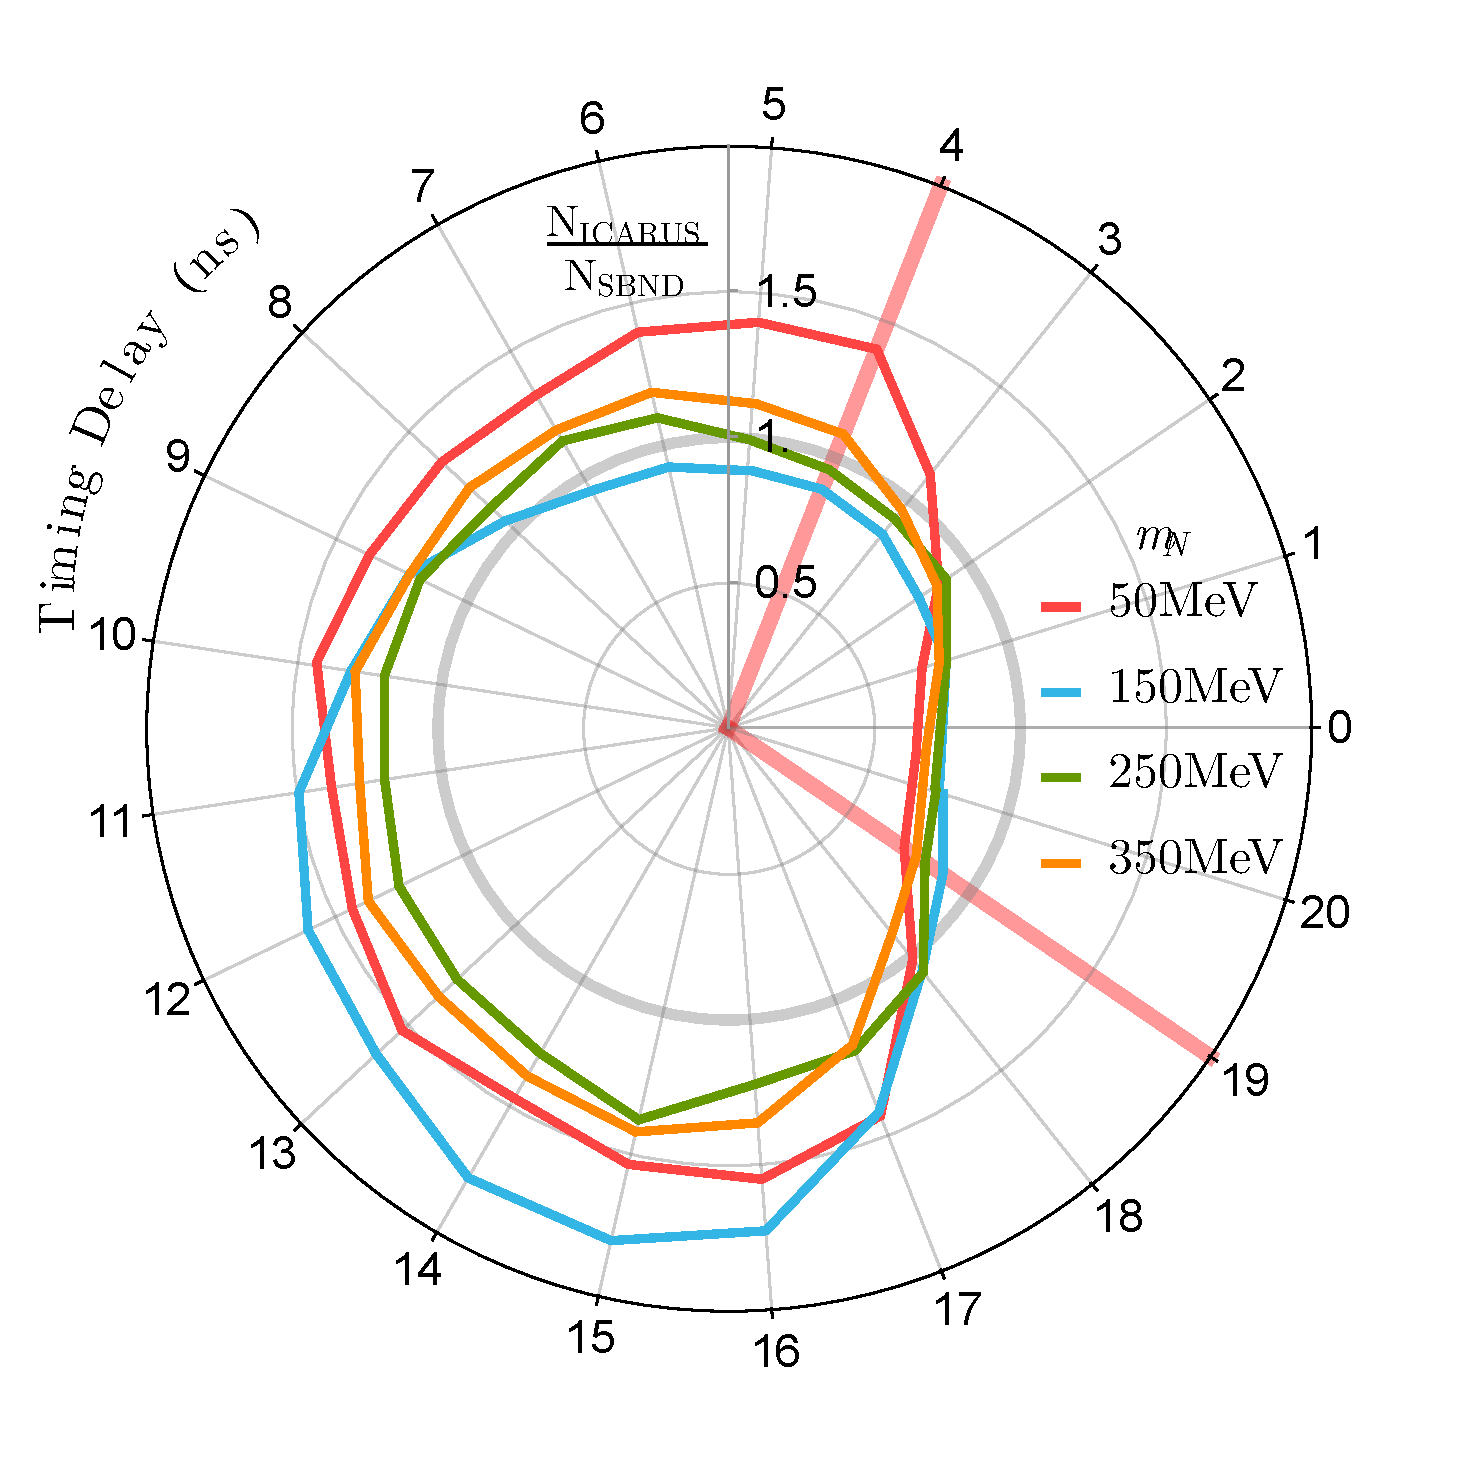
\includegraphics[width=\textwidth]{figures/ICARUS_the_great.pdf}
\end{subfigure}%
~
\begin{subfigure}[t]{0.5\textwidth}
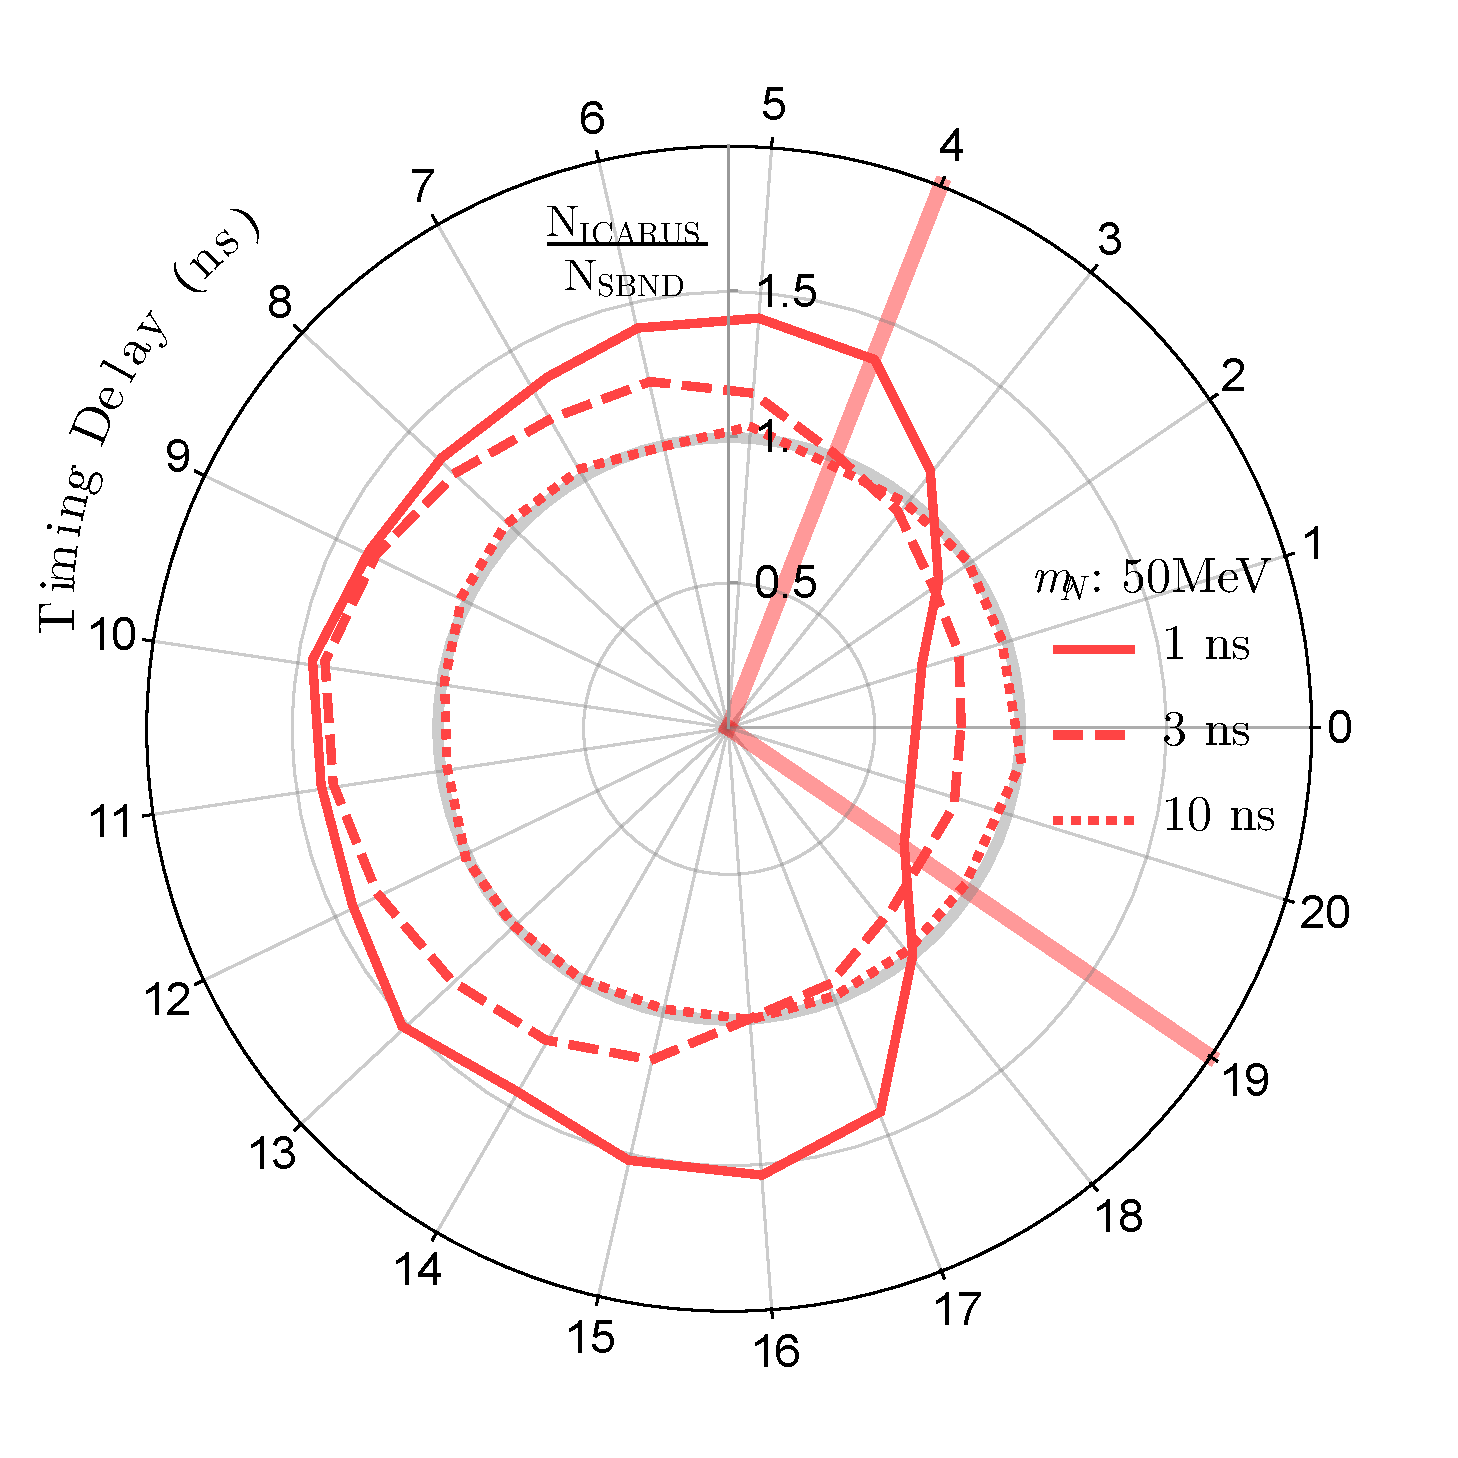
\includegraphics[width=\textwidth]{figures/ICARUS_the_great2.pdf}
\end{subfigure}
\caption{\label{fig:icarus_the_great}
\emph{Left: }Ratio of temporal shape of $\ster \rightarrow \nu_\alpha e^+ e^-$ events in ICARUS to SBND after scaling out $1/R^2$ flux dependence. If events were due to an unknown background with a fixed time delay after the neutrino beam, one would expect the ratio to be a constant value of 1 (shaded grey ring). As the steriles have to travel approximately 6 times further to ICARUS than SBND, increasingly higher energy sterile neutrinos can leave the beam-bucket (red arc) and populate the inter-bucket region leading to the distinct signature. This assumes a timing resolution of 1ns. \emph{Right: } The same as left for fixed 50 MeV sterile neutrino with 1ns (solid), 3ns (dashed) and 10ns (dotted) timing resolution showing the decreasing effect on the ratio.   }

\end{figure}

If the timing resolution is sufficient such the signal is indeed verified as
originating outside the BNB beam bucket timing, the final step would be to use
a combined energy and temporal analysis to extract measurable parameters such
as $m_\ster$. Elementary special relativity tells us that for an arrival time delay (behind a
luminal or near luminal particle) over a distance $L$ denoted by $\Delta T$,
the mass of a sterile neutrino with an energy $E$ can be reconstructed as 
%
\[ m_{\ster} = E\sqrt{1-\frac{1}{\left(1+\frac{c\Delta T}{L}\right)^2}}. \]

To determine the prospects for measuring $m_{\ster}$ using this information we
have generated Monte Carlo event data tagging each event by an arrival time.
We account for a systematic uncertainty associated with the time measurement as
well as the energy reconstruction. We smear energy to represent detector
effects as described above, and additional smear the time of each event with a
finite time resolution of $\sigma_T  \approx 1$ for SBND and ICARUS. As the
absolute timing of the event is not known, only the relative timing since the
last bucket, $\Delta T$, one can obtain up to 81 degenerate solutions for the
sterile neutrino mass from any given event depending on the placement in the spill
structure. By only studying the initial few buckets one can alleviate the
problem, however, it also reduces the signal statistics by $\mathcal{O}$(0.01)
and so all leading and trailing edge effect information is ignored in this analysis.
We utilise the same test Monte Carlo analysis and test statistic as used in the temporal analysis
above, expanded to include a binned energy spectra. The reconstructed mass defined
as the mass which minimises the test statistic $t_m$. 

The results of this analysis can be found in \reffig{fig:tof_scatter} for energy only (dashed black lines) and for energy and time-of-flight combined (coloured bands), for one leptonic $\ster \rightarrow \nu e^+ e^-$ (left)  and one semi-leptonic $\ster \rightarrow e^\pm \pi^\mp$ (right) channel. Shown are the 1 and 2 $\sigma$ ranges of reconstructed sterile neutrino mass as a function of true simulated mass. In the case of the 2-body $\ster \rightarrow e^\pm \pi^\pm$ channel, resolution of approx 45 MeV at 2$\sigma$ level is achievable for the entire range of sterile neutrino mass allowed. We estimate the $\ster\rightarrow \mu^- \pi^+$ channel would be approximately 10\% better due to the better energy resolution of muons in LAr. Temporal information only trivially improves the situation in comparison to energy only, as the exact parent kinematics can be reconstructed, limited only by detector resolution. In contrast when one considers the 3-body leptonic $\ster \rightarrow \nu e^+ e^-$ channel, we no longer have full reconstruction of the parent sterile neutrino kinematics so the achievable resolution is less. Here the addition of timing information has a much larger effect, almost halving the 2$\sigma$ mass range from ~300 MeV to ~150 MeV for wide region of parameter space.



\begin{figure}[t]
\center
%\begin{subfigure}[t]{0.485\textwidth}
%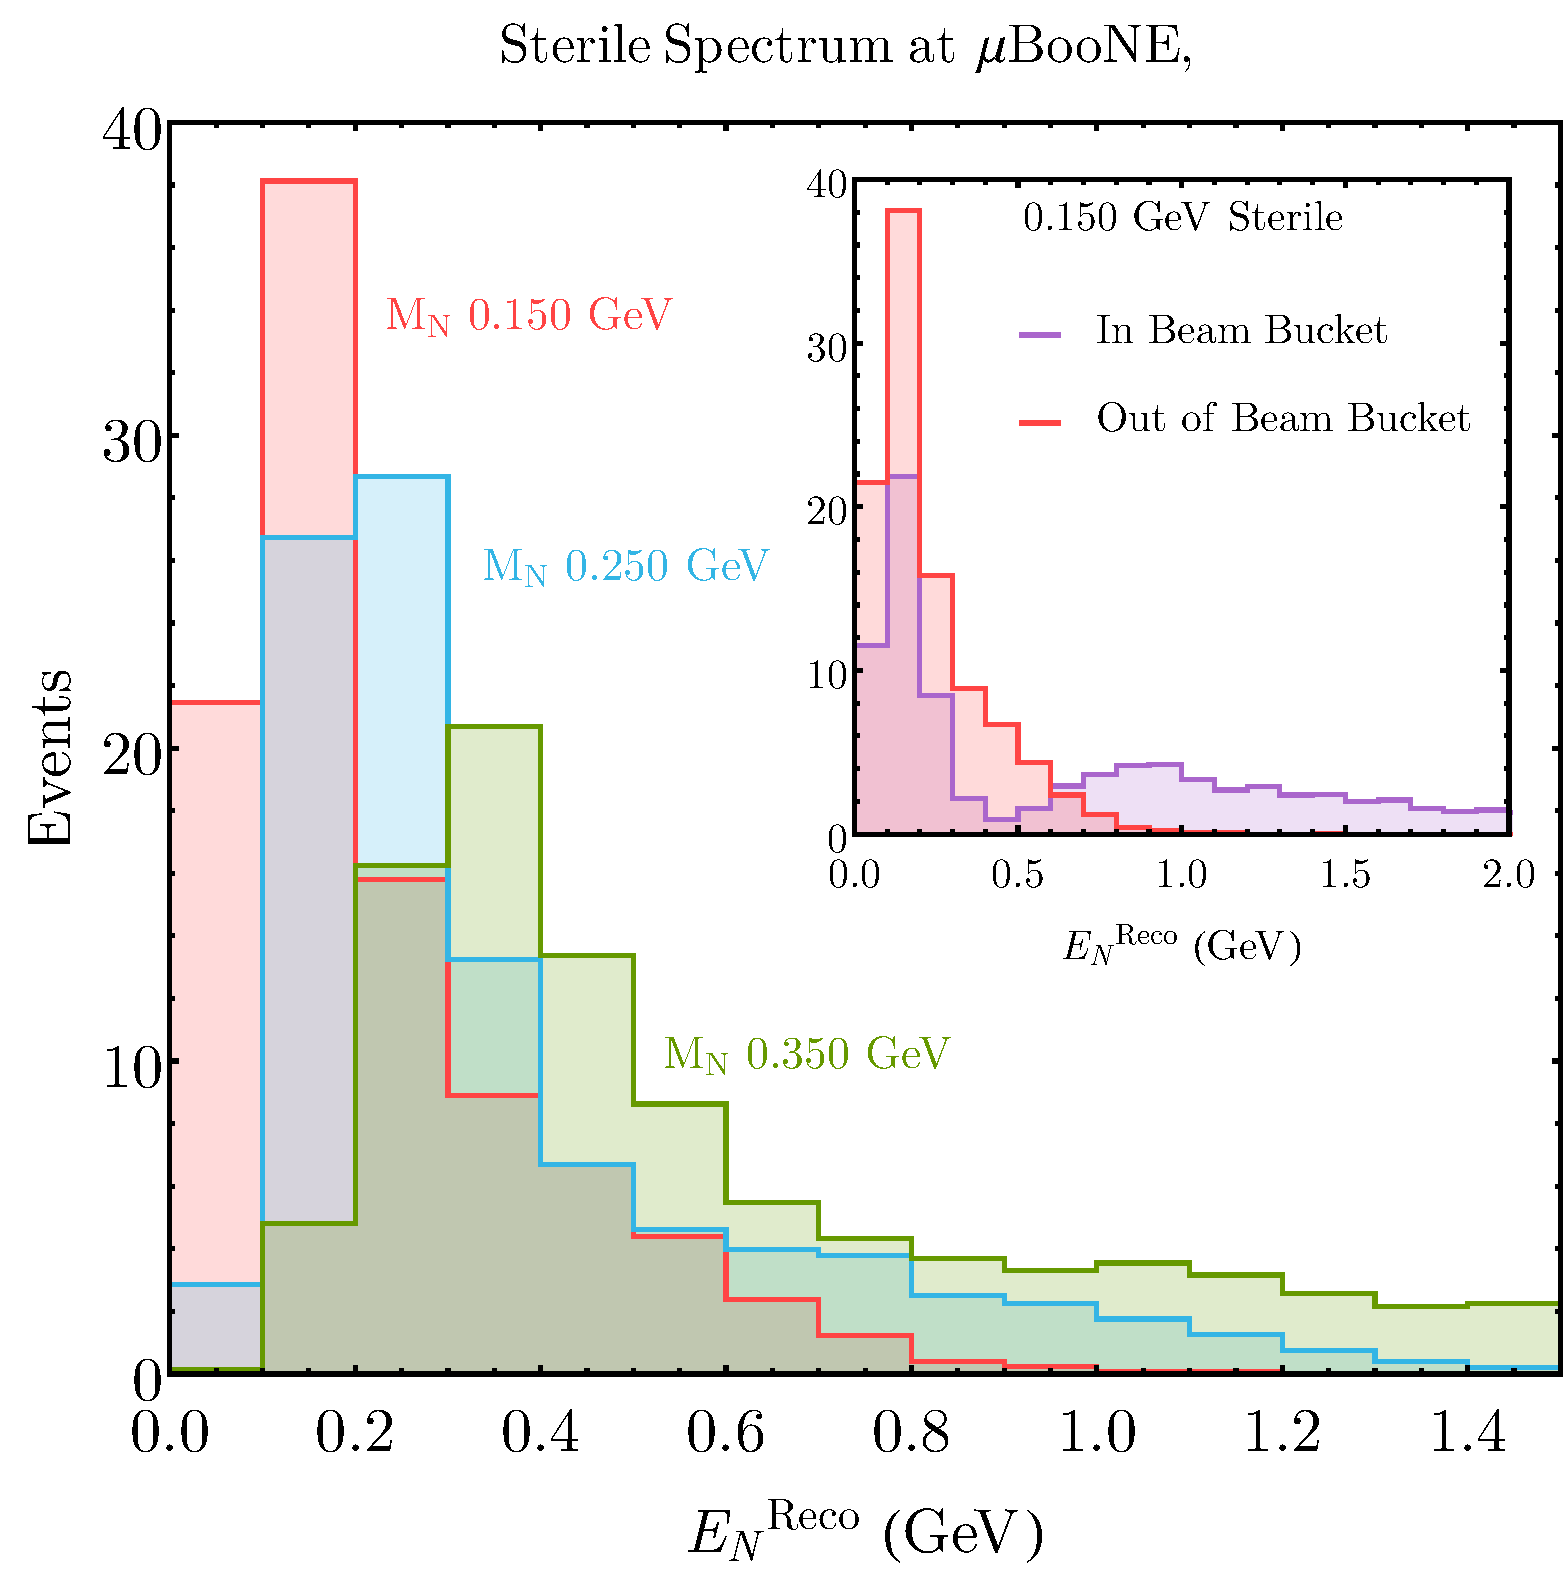
\includegraphics[width=\textwidth]{figures/sterilecomparason.pdf}
%\end{subfigure}%
\begin{subfigure}[t]{0.5\textwidth}
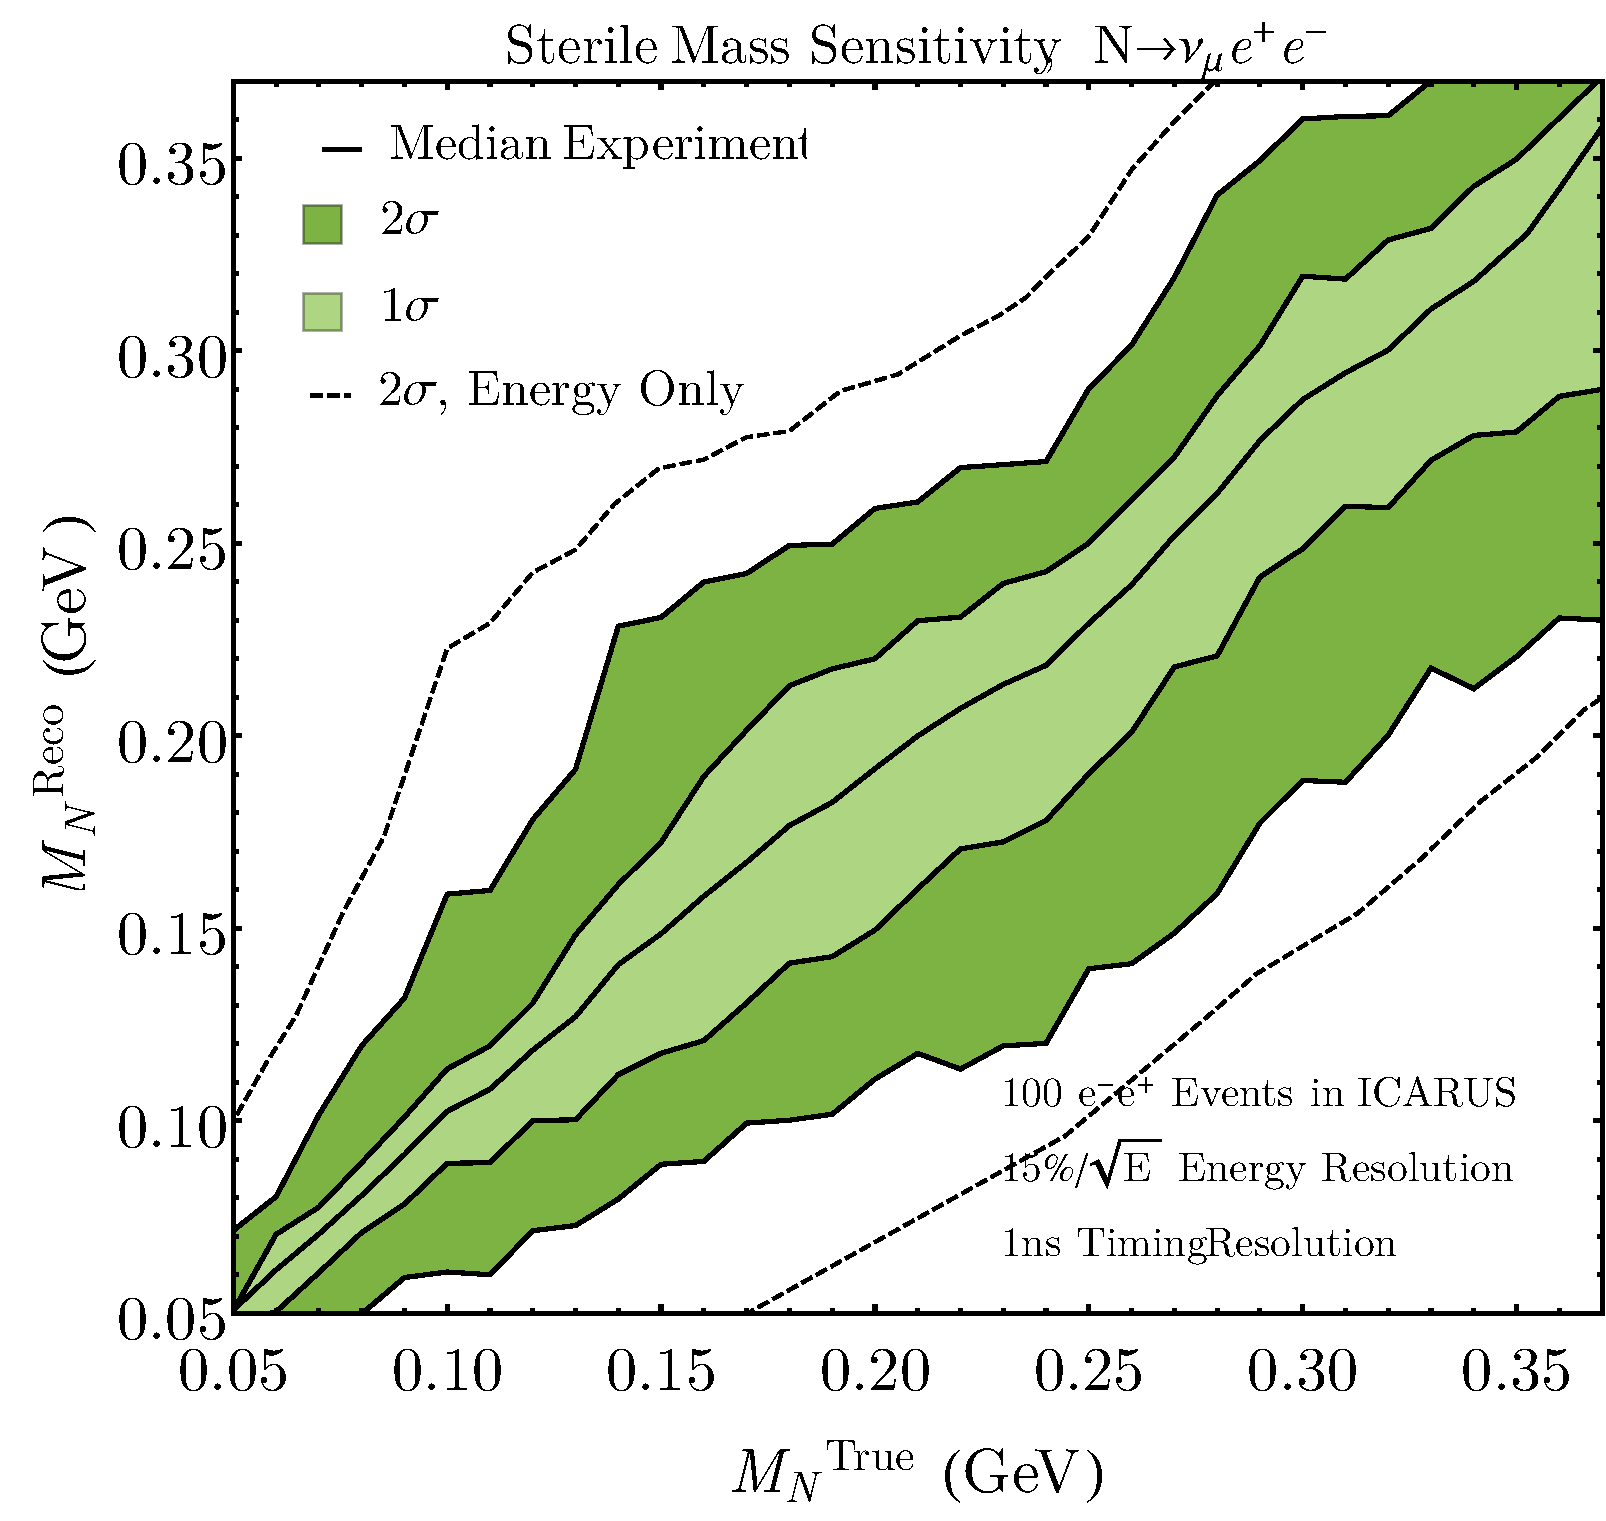
\includegraphics[width=\textwidth]{figures/icarus_mass_sensitivity_ee.pdf}
\end{subfigure}%
~
\begin{subfigure}[t]{0.5\textwidth} %0.515
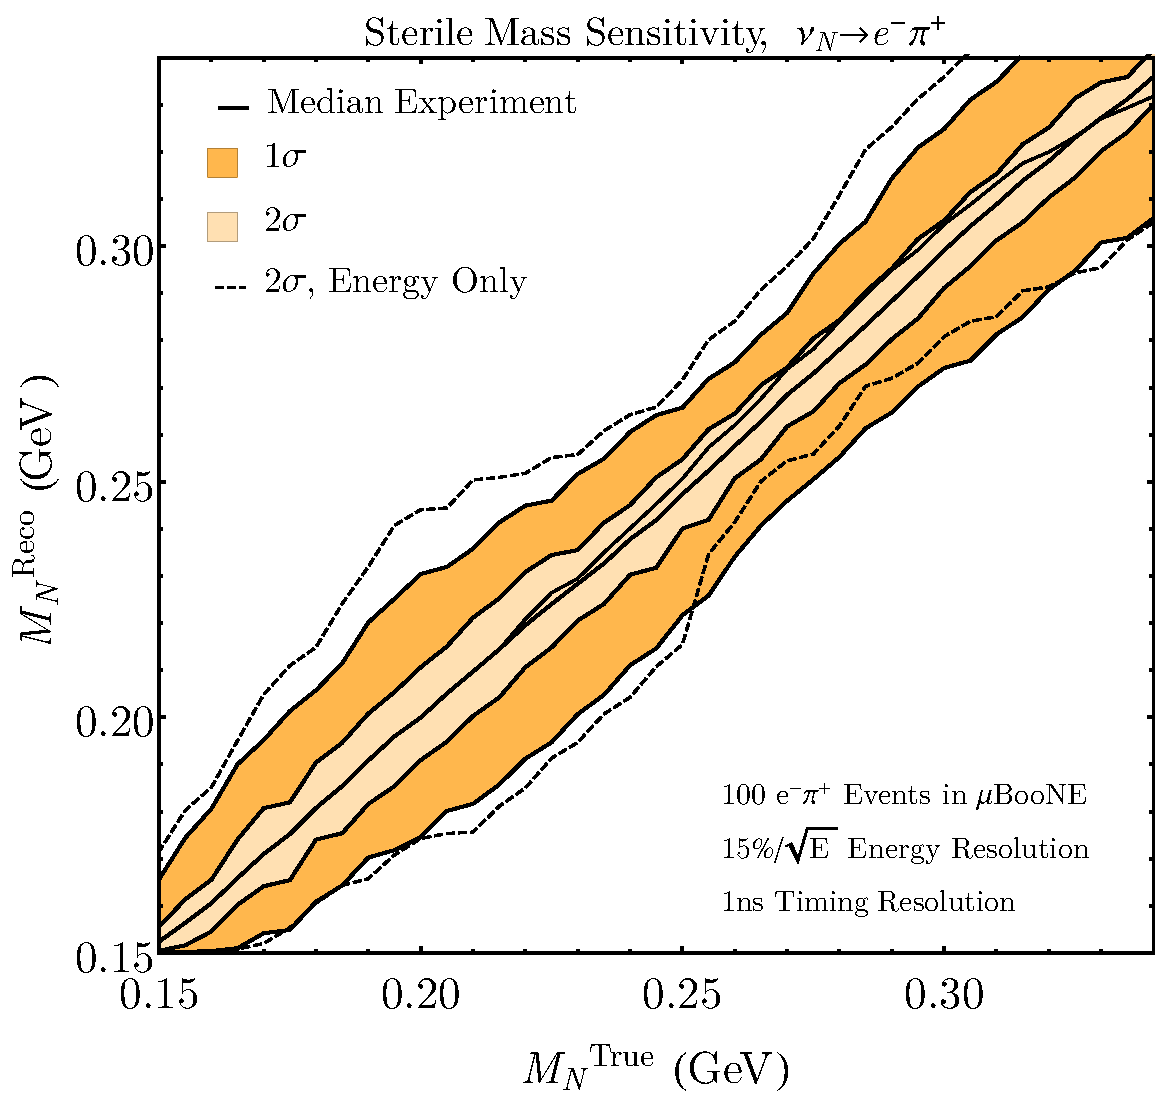
\includegraphics[width=\textwidth]{figures/icarus_mass_sensitivity.pdf}
\end{subfigure}

\caption{\label{fig:tof_scatter}
%Left: The spectral differences in total visible energy, $E_N^\text{RECO}
%\equiv E_{e^-}+E_{\pi^+}$, for sterile masses of 150, 250 and 350 MeV. Insert
%shows the stark differences between events falling within the beam bucket
%window and without.
	\emph{Left:} Sensitivity to sterile neutrino mass in $\ster \rightarrow
\nu_\alpha e^+ e^-$ channel from reconstructed sterile neutrino energy only (Dashed
lines) as well as when one includes additional time-of-flight information
(Green shaded regions).  Energy alone does poorly in identifying the parent
mass, especially at low masses, but the addition of timing information allows
for significantly better resolution.  \emph{Right:} Same as left but for $e^-
\pi^+$ channel. Resolution of approx 45 MeV at 2$\sigma$ confidence is
achievable for the entire range of sterile neutrino mass allowed if 100 events are
observed. Note that energy alone has significantly better resolution due to
lack of missing-energy in the final state.}
\end{figure}


\section{\label{sec:conclusions}Conclusions}

In this paper, we have studied the capabilities of the Fermilab Short-Baseline
Neutrino program to constrain possible decays of heavy MeV scale sterile
neutrinos. This is a complementary study to the standard light oscillating
sterile neutrino searches that requires no additional detector or beam modifications.
These states would naturally be produced in the Booster Neutrino Beam from
mixing-matrix suppressed meson decays. To make a fair assessment of the
potential to constrain these models, we have performed a cut-based analysis of
the dominant backgrounds and signals and shown that in conjunction with
sufficiently accurate timing measurements, $\approx 1$ ns, high levels of
background suppression can be expected resulting in low-background searches in
all channels studied. Using these background estimates, we have performed a
sensitivity analysis to the parameters of the minimal extension of the SM with
a novel sterile neutrino, $|U_{e4}|$ and $|U_{\mu4}|$ . 
%
We find that SBN can extend the current bounds over most of the parameter space
under consideration. Each detector plays a distinct role in the process:
MicroBooNE is already collecting data and has the potential to observe a signal
first guiding further studies; SBND provides the bulk of the statistics due to
its proximity to the BNB; and ICARUS, at 600m downstream, is vital for
exaggerating the timing delay associated with heavy propagating particles,
which can be used for background suppression and comparative analyses with
events from SBND.
%
We have also motivated searches for non-minimal models, which in particular
could lead to observable decays over a wide range of parameter space which is
conventionally excluded by theoretical assumptions on the decay rates
themselves. We argue that some of these decay channels are actually
\emph{unconstrained} by similar experiments, and show that the SBN could place
the first direct bounds on these processes.
%
We highlight the phenomenological potential of accurate scintillation light
timing information in LArTPCs. We argue that a sufficiently good timing
resolution, around $3$ ns, can play a key role in the reduction of backgrounds
thanks to the sub-luminal propagation speeds of heavier sterile neutrinos
syncopating the beam-related backgrounds and signal events. In addition, we
have shown that the inclusion of timing information in the reconstruction of
the sterile neutrino's mass can improve the sensitivity from an energy-only analysis as
well as providing a method to definitively prove that an observed excess is due
to the propagation and subsequent decay-in-flight of a heavy particle and not
in line with beam-related background.
%

\acknowledgments

We would like to thank Andrezj Szelc for his input at various stages of this
work, and also to Jonathan Asaadi for helpful discussions and encouragement at
the start of this project.

This work has been supported by the European Research Council under ERC Grant
``NuMass'' (FP7-IDEAS-ERC ENC-CG 617143), \newtext{PB}{by the European Union FP7
ITN-INVISIBLES (Marie Curie Actions, PITN-GA-2011-289442), as well as from the
H2020 funded ELUSIVES ITN (H2020-MSCA-ITN-2015, GA- 2015-674896-ELUSIVES) and 
InvisiblePlus (H2020-MSCA-RISE-2015, GA-2015-690575-InvisiblesPlus).}

\appendix

\section{\label{app:decayrates}Decay rates in the minimal model}

The dominant visible decay for sterile neutrinos with masses below the pion
mass is into an electron positron pair. The total rate can be express as
%
\begin{align*} \Gamma\left(\ster\to \nu_\alpha e^+e^-\right) =
\frac{G_\text{F}^2m_\ster^5}{96\pi^3}\left|U_{\alpha 4}\right|^2&\left[\left( g_Lg_R + \delta_{\alpha e}g_R\right)I_1\left(0,\frac{m_e}{m_\ster}, \frac{
m_e}{m_\ster}\right)\right.\\ 
&\left.\qquad + \left(g_L^2 + g_R^2 + \delta_{\alpha e}(1+2g_L)\right)I_2\left(0,\frac{m_e}{m_\ster},\frac{m_e}{m_\ster}\right)\right],  \end{align*}
%
where $g_L = -1/2 + \sin^2\theta_\text{W}$, $g_R = \sin^2\theta_\text{W}$ and
% 
\begin{align*} I_1(x,y,z) & =12 \int_{(x+y)^2}^{(1-z)^2}
\frac{ds}{s}(s-x^2-y^2)(1+z^2-s)\sqrt{\lambda(s,x^2,y^2)}\sqrt{\lambda(1,s,z^2)},\\
I_2(x,y,z)& =24yz\int_{(y+z)^2}^{(1-x)^2}\frac{ds}{s}\left(1+x^2-s\right)\sqrt{\lambda\left(s,y^2,z^2\right)}\sqrt{\lambda\left(s,y^2,z^2\right)},\\
\lambda(a,b,c) &= a^2+b^2+c^2 - 2ab-2bc-2ca.  \end{align*}
%
The decays into a charged lepton and a pion are given by 
%
\[ \Gamma\left(\ster\to l^\pm\pi^\mp\right) =
\left|U_{l4}\right|^2\frac{G_\text{F}^2f_\pi^2 |V_{ud}|^2
m_\ster^3}{16\pi}I\left(\frac{m_l^2}{m_\ster^2} ,
\frac{m_\pi^2}{m_\ster^2}\right) , \] 
%
with \[ I(x,y) = \left[ \left( 1+x+y\right) \left(1+x\right) -4 x\right]
\lambda^\frac{1}{2}\left(1,x,y\right).  \]
%
For $N\to e^\pm\pi^\mp$ the kinematic function $I(x,y)$ produces only weak suppression ($I(x,y)\geq 0.5$) for sterile  neutrino masses above $m_\ster\gtrsim 150$ MeV, whilst for $N\to
\mu^\pm\pi^\mp$ the equivalent threshold is $m_\ster\gtrsim 270$ MeV.

\section{Potential Backgrounds\label{app:bg}}
%In order to estimate the effect of expected backgrounds on the sensitivity we
%have performed a Monte-Carlo analysis using the neutrino event generator GENIE
%\cite{Andreopoulos:2009rq}. This provides us with generator level information
%about the kinematics of the beam-driven backgrounds, with rates normalised off
%expected NC and CC inclusive values as published in the SBN proposal. Energy
%and angular smearing is then implemented to allow for approximate estimates of
%the effects of detector performance to the level necessary for this analysis,
%without the need for a full GEANT detector simulation. Energies are smeared
%according to a Gaussian distribution around their true MC energies, with a
%relative variance $\sigma_E/E = \xi/ \sqrt(E) $, where $\xi$ is a detector
%dependant resolution.  For this study we take the energy resolution for EM
%showers, muons and protons to be 15\%, 6\% and a conservative 15\%
%respectively, alongside the angular resolution of LAr to be $1.73^{\circ}$
%\cite{Antonello:2015lea}. 
%
%Of utmost importance in all studied channels is the identification of a
%scattering vertex. Any hadronic activity localized at the beginning of the
%lepton track is a smoking gun signal for beam related scattering from
%deep-inelastic or quasi-elastic scattering. Therefore any event containing one
%or more reconstructed protons or additional hadrons is rejected outright. For
%counting this proton multiplicity we assume an detection threshold of 21 MeV
%on proton kinetic energy in liquid Argon \cite{Acciarri:2014gev}, after
%smearing.  Background events that contain less than this and events that do
%not contain any protons, such as events originating from coherent pion
%production, remain a viable background and further rejection must come from
%the kinematics of the final state particles only.
%
%All two body visible decays discussed below have a powerful discriminator in
%the reconstructed invariant mass of the charged particle pair, e.g  $M_{l^\pm
%\pi^\mp}^2=m_l^2+m_{p^\pm}^2+ 2(E_l E_\pi - |P_l||P_\pi|\cos\theta_\text{sep})$
%for $\ster\rightarrow \pi^+ l^-$, which sum to that of the the parent sterile
%(within detector resolution), where as the background is expected form a broad
%spectra spanning the energies of incoming neutrino. Additionaly, two body
%decays allow for reconstruction of the parent sterile angle with respect to the
%beamline which is assumed to be close to on-axis, unlike the more isotropic
%backgrounds. We found $\approx 95$\% of reconstructed sterile from two bodys
%decays were below $4^\circ$ relative to the beamline and we cut all events
%greater than this. 
%
\subsection{$\ster \rightarrow \mu^\pm \pi^\mp$ and $\ster \rightarrow e^\pm \pi^\mp$   }

The dominant backgrounds to the sterile neutrino decays we are interested in will be
genuine $\pi$-lepton production associated with the neutrino beam. So-called
CC1$\pi^+$ events are defined as the associated production of a charged pion
from the standard CC process which produces a lepton. These events can be
produced incoherently, often with large hadronic activity, or from coherent
scattering, where the neutrino scatters from the whole nucleus. These coherent
interactions tend to produce more forward decay products and will be another
significant source of backgrounds. Coherent cross-sections for these processes
have been studied in MiniBooNE \cite{Wascko:2006tx}, \minerva
\cite{Eberly:2014mra} and lately T2K and cross-sections appear to agree with
Monte Carlo calculations based on the Rein-Sehgal model \cite{Rein:2006di,
Rein:1982pf}.  Such a low $Q^2$ process tends to favour daughter pions and
muons that are forward going, kinematically very similar to decays in flight,
as well as no observable nuclear activity and as such are a potent
background.\\ 

The expected numbers of $e \pi$ events in the SBN detectors is significantly
smaller than that of the $\mu \pi$ channel, as the fraction of intrinsic
$\nu_e$ in the BNB beam is of $\mathcal{O}(1\%)$ level in comparison to
$\nu_\mu$. However, there will also be additional backgrounds to the $e \pi$
channel originating from the dominant $\nu_\mu$ beam. CC $\nu_\mu$ events which
contain an additional photon $(\mu+\gamma)$, or 1 reconstructed photon from a
$\pi^0$ decay, have the potential to be be mis-identified as an $(\pi e)$
event, provided the muon has a sufficiently short track length, $<$ 0.5 m, in
order to mimic a $\pi^-$. Additionally the photon must be mis-identified as an
electron, with an efficiency of 94\%, and furthermore, must convert to an
$e^+e^-$ pair close enough to the interaction vertex as so there is no visible
gap. Thus we accept 6\% of all CC $\mu+\gamma$ events whose photon converts
within 3cm, and whose muon track length is less than 0.5m. Combined with the
rejection of events with any vertex activity, this reduces the number of
background events to below that expected from intrinsic CC $\nu_e$ pion
production. As energy resolution for EM showers is lower than muons, the
invariant mass cut is less powerful requiring all events have an invariant mass
below 500 MeV. 

Additional kinematic cuts are selected to further separate the kinematics of
decay and scattering events. A cut on the opening angle between lepton on
meson, $\theta_{l \pi} < 40^\circ$ as well as individual emission angles,
$\theta_{l,\pi} < 80^\circ$ further reduces the potential background. The total
effect of all these cuts reduce the background events from 1,153,090 in SBND to
approximately 323 events for $\mu^- \pi^+$.  \reffig{fig:mu_pi_cutflow}
pictorially shows this background rejection capability of LAr as each
additional cut is implemented in \muboone, in comparison to a 350 MeV sterile neutrino
decay. The $e^- \pi^+$ channel is one of the cleanest channel under
consideration, with 9,223 events in SBND reducing to 22 expected events post
cuts, and with \muboone\ and ICARUS expecting $\mathcal{O}(1)$ events from beam
driven backgrounds.


\subsection{$\ster \rightarrow \nu_\alpha e^+ e^-$ and $\ster \rightarrow \gamma \nu_\alpha$ }

A sufficiently boosted, and thus overlapping, $e^+e^-$ pair is topologically
indistinguishable from a converted photon in a LAr detector. Additional,
non-topological measures such as the rate of energy loss, $dE/dx$, is also
identical to a pair-converted photon. Thus we split this channel into two sub
categories, when the $e^+e^-$ is overlapping and photon-like, defined to be all
events whose angular separation is $\leq 3^\circ$\cite{Spitz:2011wba} and all
remaining separable two track events. The opening angle between the $e^+e^-$ in
a photon pair production scales roughly as $\approx m_e/E_\gamma$, with
$3^\circ$ corresponding to 100 MeV and used as a lower bound on energy. These
backgrounds are also applicable to the $\ster \rightarrow \nu_\gamma
\nu_\alpha$ channel.\\ 

Any standard process producing a lone stray photon is thus a possible source of
backgrounds for the photon-like $e^+e^-$ channel. The predominant source of
this in all three SBN detectors is the decay of a neutral pion in which a
single photon is not resolved or escapes the fiducial volume. This background,
however, is relatively isotropic in distribution and of lower energy that the
signal, in stark contrast to the very forward signal. Thus we apply a cut on
visible photon energy, $E_\gamma \geq 300 $ MeV and angle of the observed
photon to the beamline, $\theta_\gamma \leq 5^\circ$. In conjunction with the
requirement that no vertex activity is recorded, this reduced the number of
expected events from 42,580 to 176 events in SBND, while retaining a signal
efficiency of 93\%.

For the opposite scenario both daughter electrons have a well defined, and
large, separation and thus can cleanly be identified as two distinct single
electron showers. There are no significant processes that produce high energy,
distinguishable $e^+e^-$ pairs in a standard neutrino beam.  Instead the
majority of the backgrounds are due to misidentifying photons, which are
abundant, as electrons. This can either be a single photon alongside a CC $e^-$
event or the more common NC $\pi^0$ production in which both of the underlying
photons are mis-identified as electrons. As both of these backgrounds require
the photons to mimic electrons originating from a single decay vertex, we also
require that all photons pair convert within 3cm of the start of the electron
track in the case of CC $\nu_e$ backgrounds, or both photons convert within 3cm
of each other in the case of NC $\pi^0$ backgrounds. Further more, each event
passing the above cuts is rejected with a 94\% efficiency using measurements of
the rate of energy loss, $dE\/dx$. All remaining events are kept as
backgrounds. To further reject backgrounds we apply a cut on angle of
separation between the distinct $e^-e^-$ tracks of $\theta_\text{sep}\leq 40
^\circ$ and total energy, $E_{e^+}+E_{e^-} \geq 100$ MeV. This reduces the
number of expected backgrounds from 173 events to 5 events in SBND. 

\subsection{$\ster\rightarrow \pi^0 \nu_\alpha$}

Although a sub-dominant decay mode when steriles mix with electrons alone, when
one considers non-zero $\vert U_{\mu4}\vert^2$ the branching ratio of $\ster
\rightarrow \nu_\mu \pi^0$ becomes dominant for a mass window $\approx 140
\rightarrow 240$ MeV. There is no known experimental publication of $\ster
\rightarrow \nu_\alpha \pi^0$ in the literature, mainly due to the large
expected backgrounds. Single neutral pions are produced in great numbers at the
three SBN detectors, so the lack of any nuclear recoil is crucial in
eliminating the incoherent neutral pion production background. As the $\pi^0$
itself is not visible, we focus on the reconstructed pion energy and angle,
inferred from measuring the resultant photons energy and angle, smeared as
usual to model detector effects. Only events in which both photons convert
inside the fiducial volume are accepted. SBND expects 127,211 $\pi^0$ events,
of which $\approx 602$ survive all cuts with a signal efficiency of 32\% for a
sample 350 MeV sterile neutrino. \\ 

To summarise, we collect the total numbers of beam-induced background events
expected at the three SBN below in \reftab{tab:Rates}, both before and after we
apply all visible vertex and kinematic cuts as described above. One can see
that LAr provides an impressive level of background rejection, with \muboone
and ICARUS being close to backgroundless in many channels, and SBND expecting
only $\mathcal{O}(100)$ events in all channels.

\begin{table}[t]
\centering
\begin{tabular}{ l | l |  l | l |  }
	Signal Channel & Events @ SBND & \muboone\ & ICARUS \\
\hline\hline
$\mu^\pm \pi^\mp$ &  1,530,900  & 98,013 & 164,716\\
													  w/ Cuts &323 & 27 & 46 \\ \hline
$ e^\pm \pi^\mp$ &  9,228  & 784 & 1,317\\
													  w/ Cuts &22 & 2 & 3 \\ \hline
$ \nu_\alpha \pi^0$ &   127,217 & 10,813 & 18,172\\
													  w/ Cuts &603 & 51 & 86 \\ \hline
$ e^+e^- \text{ (Separate)} $ & 173 & 14 & 24\\
													  w/ Cuts &5 & 0.3 & 0.5\\ \hline
$ e^+ e^- \text{ or } \gamma \text{ (Photon-like)}$ &  42,580 & 3,620 & 6,082\\
													  w/ Cuts &176 & 46 & 110 \\ 
 \hline \hline

\end{tabular}

\caption{\label{tab:Rates} A summary of the main sources of backgrounds for
each channel studied, before and after spectral and particle ID cuts are
applied as discussed in \refapp{app:bg}. }

\end{table}


\subsection{Non-Beam related backgrounds}

Cosmogenic backgrounds are a potential source of background for any analysis at
SBN. In the case of cosmic muons, \icarus\ expects to see approximately $2.5
\times 10^{6}$ cosmic events in the 211 second beam spill, and are reduced to
approximately 5 events expected after utilizing the spill structure,
scintillation light patterns and cuts on $\frac{d E}{d x}$
\cite{Antonello:2015lea}.  Alongside this impressive cosmic rejection, our
signal events are focused heavily along the beamline, hence we do not expect
cosmics to be a major source of background to any channel. In situ beam-off
cosmic studies will also allow potential backgrounds to be extremely well
understood by the time of an analysis such as this, are so are not included in
this analysis. 

\section{PS-191 Bound Reproduction\label{sec:ps191}}

As a consistency check of our methodology we reproduce here the bounds on
$|U_{e4}|$ and $|U_{\mu 4}|$ for sterile masses below $m_\pi$ as published by
PS-191. The detector geometry is assumed to be $6\text{m} \times 3\text{m}
\times 12 \text{m}$ and was located 128m downstream of the Beryllium target
using 19.2 GeV protons from the PS proton beam.  Fluxes of all neutrinos
produced from pion sources at PS-191 were obtained from \cite{ps191THesis}. No
accurate kaon sources could be obtained and as such only low mass bounds are
reproduced here. It must be noted that PS-191 ignored all neutral current
contributions to $\ster \rightarrow \nu_\alpha e^+ e^-$ and assumed the sterile
neutrinos were Dirac particles; the effect of this is that the bounds published
are not directly comparable to the minimal model discussed above, and must be
scaled appropriately. The bounds reproduced are in good agreement with published
data.

\begin{figure}
			  \centering
			 
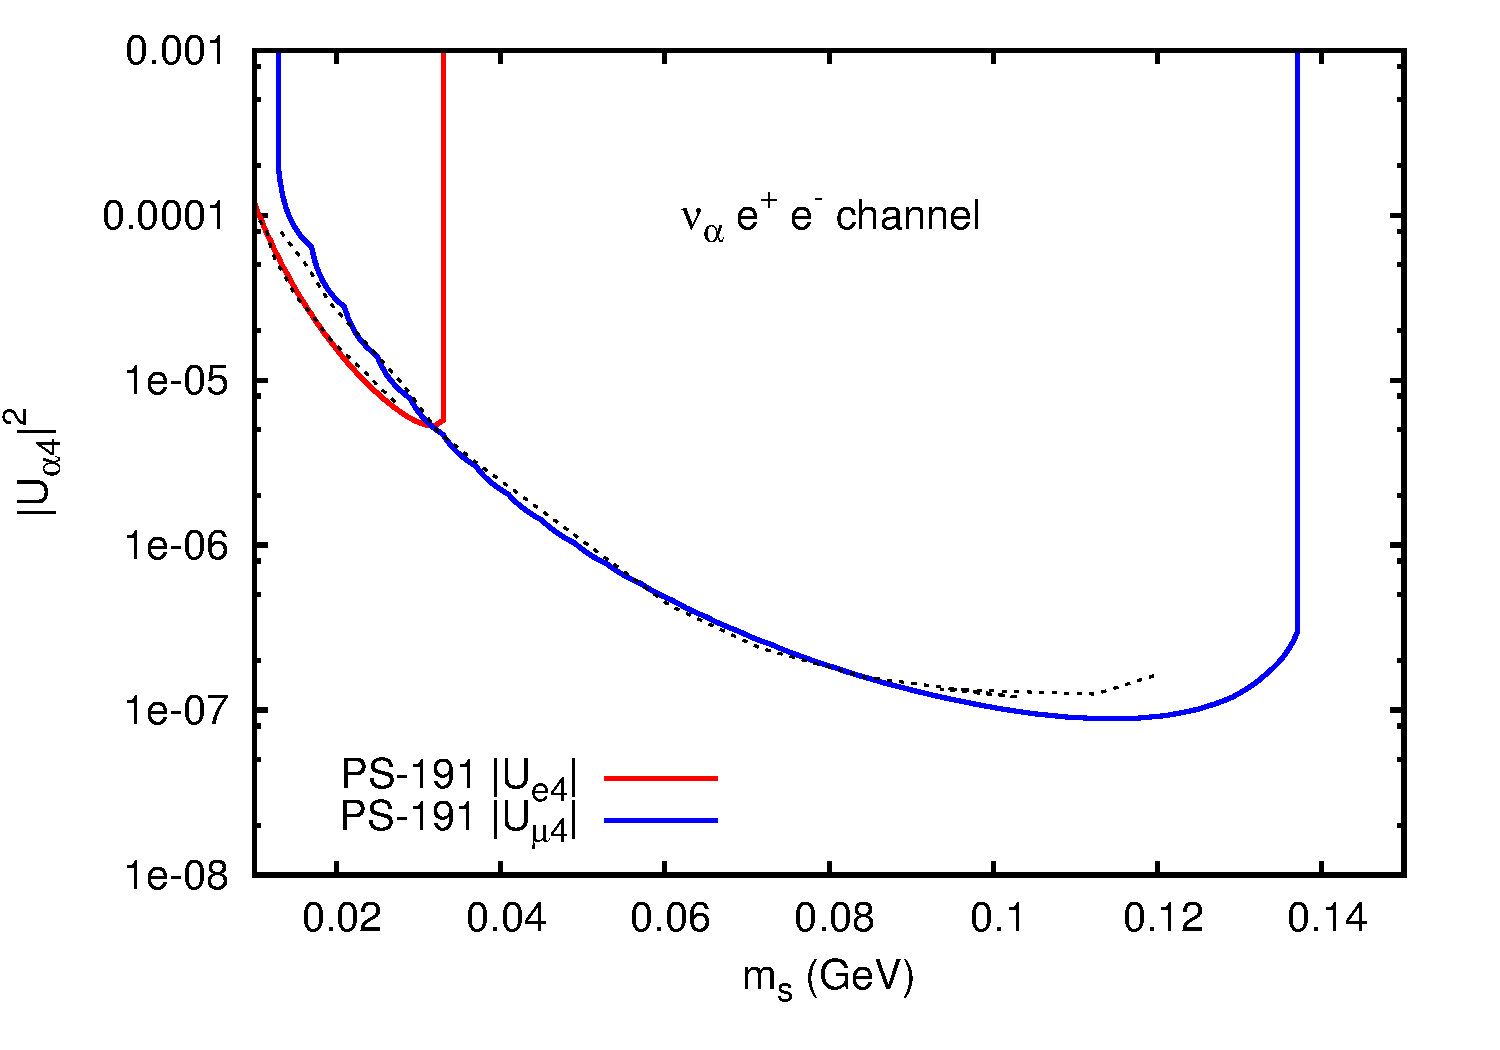
\includegraphics[width=0.5\textwidth]{figures/PS-191_test.pdf}

\caption{\label{fig:ps191test} Estimated bounds on $|U_{e4}|^2$ and $|U_{\mu
4}|^2$ for a Dirac heavy sterile neutrino decaying to $\nu_\alpha e^+ e^-$ at
PS-191. The dotted black lines are the 90\% C.L results as published by PS-191,
and the blue and red curves are the results of our simulation for $0.86 \times
10^{19}$ POT.}

\end{figure}

%\newpage
%
%\section{To do list}
%
%\begin{enumerate}
%
%\item Do a bit more checking that the `unobserved' channels are indeed unobserved. 
%
%\item Are the effective model decay channels unbounded? \newtext{PB}{I think } \refref{Aparici:2009fh} \newtext{PB}{goes some of the way to placate my worries: they show bounds for their operators, and in our region of interest there is nothing killer (I think).}
%
%\item Turn on $U_{\tau 4}$,$U_{\mu 4}$ and $U_{e4}$ simultaneously. Think of
%how we can push the analysis beyond the obvious by using flavour effects. Also
%look at ratios of channels and ratios of events to see if we can get any
%(broken) degeneracies that could actually be interesting \emph{i.e} SNO style
%complementary measurements.
%
%\item \newtext{MARK}{Working on} Make nice version of branching ratio plot.
%Need to make prettier. \sout{Also, we probably need to cut it off at
%$M_\ster\lesssim 500$ MeV, there are other decays allowed between 0.5 and 1 GeV
%(with $\eta$ and $\rho$)}.
%
%\item \newtext{MARK}{Working on} Think if there's a nice plot showing the
%sterile effect on our fluxes.
%
%\end{enumerate}
%

%%%%%%%%%%%%%%%%%%%%%%%%%%%%%%%%
%%%%%%%%%%%%%%%%%%%%%%%%%%%%%%%%
%%%%%%%%%%%%%%%%%%%%%%%%%%%%%%%%

\bibliographystyle{apsrev4-1}
\bibliography{lib}{}

\end{document}

